\documentclass[aspectratio=169,11pt,hyperref={colorlinks=true}]{beamer}
\usetheme{boxes}
\setbeamertemplate{navigation symbols}{}
\definecolor{ibm}{RGB}{70,107,176}
\setbeamercolor{titlelike}{fg=ibm}
\setbeamercolor{structure}{fg=ibm}
\hypersetup{colorlinks,urlcolor=ibm}
\setbeamertemplate{footline}[frame number]
% Inserting graphics
\usepackage{graphicx}
% Side-by-side figures, etc
\usepackage{subfigure}
% Code snippits
\usepackage{listings}

\usepackage{lmodern}
% Color stuff
\usepackage{color}
\usepackage{amsmath}
\usepackage{tabu}
\usepackage{amssymb}
\usepackage{empheq}
\usepackage[braket, qm]{qcircuit}
\usepackage{tikz}
\usetikzlibrary{snakes,arrows,shapes}
\usepackage{gensymb}
\newcommand\RBox[1]{%
  \tikz\node[draw,rounded corners,align=center,] {#1};%
}
\usepackage{hyperref}
%\usecolortheme{buzz}
%\usecolortheme{wolverine}
%\usetheme{Boadilla}
\usepackage[T1]{fontenc}

\definecolor{mygreen}{rgb}{0,0.6,0}
\definecolor{mygray}{rgb}{0.5,0.5,0.5}
\definecolor{mymauve}{rgb}{0.58,0,0.82}

\lstset{%
  backgroundcolor=\color{white},   % choose the background color; you must add \usepackage{color} or \usepackage{xcolor}
  breakatwhitespace=false,         % sets if automatic breaks should only happen at whitespace
  breaklines=true,                 % sets automatic line breaking
  captionpos=b,                    % sets the caption-position to bottom
  commentstyle=\color{ibm},  % comment style
  extendedchars=true,              % lets you use non-ASCII characters; for 8-bits encodings only, does not work with UTF-8
  keepspaces=true,                 % keeps spaces in text, useful for keeping indentation of code (possibly needs columns=flexible)
  keywordstyle=\color{blue},       % keyword style
%  otherkeywords={*,...},           % if you want to add more keywords to the set
  numbersep=5pt,                   % how far the line-numbers are from the code
  numberstyle=\tiny\color{mygray}, % the style that is used for the line-numbers
  rulecolor=\color{black},         % if not set, the frame-color may be changed on line-breaks within not-black text (e.g. comments (green here))
  showspaces=false,                % show spaces everywhere adding particular underscores; it overrides 'showstringspaces'
  showstringspaces=false,          % underline spaces within strings only
  showtabs=false,                  % show tabs within strings adding particular underscores
  stringstyle=\color{ibm},   % string literal style
}


\setbeamerfont{caption}{series=\normalfont,size=\fontsize{6}{8}}
\setbeamertemplate{caption}{\raggedright\insertcaption\par}

\setlength{\abovecaptionskip}{0pt}
\setlength{\floatsep}{0pt}

\author[Matthew Treinish]{%
    \texorpdfstring{%
        \centering
        Matthew Treinish\\
        Software Engineer - IBM Research\\
        \href{mailto:mtreinish@kortar.org}{mtreinish@kortar.org}\\
        \texttt{mtreinish on Freenode}\\
        \href{https://github.com/mtreinish/quantum-compilers}{https://github.com/mtreinish/quantum-compilers}
   }
   {Matthew Treinish}
}
\date{January 17, 2020}

\title{Building a Compiler for Quantum Computers}
\begin{document}

\titlepage
\section{How to Program Quantum Computers}
\subsection{Quantum Circuits}
\begin{frame}
    \frametitle{Quantum Circuits}
    \begin{columns}
        \column{0.5\textwidth}
            \begin{itemize}
                \item Used to describe operations on a quantum computer
                \item Each row represents a bit (either classical or quantum)
                \item Shows dependency of operation
            \end{itemize}
        \column{0.5\textwidth}
            \begin{equation*}
                \Qcircuit @C=1.0em @R=0.0em @!R {
            	 	\lstick{ q_{0} : \ket{0} } & \gate{H} & \ctrl{1} & \meter & \qw & \qw & \qw\\
            	 	\lstick{ q_{1} : \ket{0} } & \qw & \targ & \qw & \meter & \qw & \qw\\
            	 	\lstick{c_{0}: 0} & \cw & \cw & \cw \cwx[-2] & \cw & \cw & \cw\\
            	 	\lstick{c_{1}: 0} & \cw & \cw & \cw & \cw \cwx[-2] & \cw & \cw\\
            	}
            \end{equation*}
    \end{columns}
\end{frame}
\subsubsection{Quantum Gates}
\begin{frame}
    \frametitle{Quantum Gates}
    \begin{itemize}
        \item Quantum gates
        \item Gates are reversible
        \item Each gate can be represented as a unitary matrix
    \end{itemize}
    \centering
    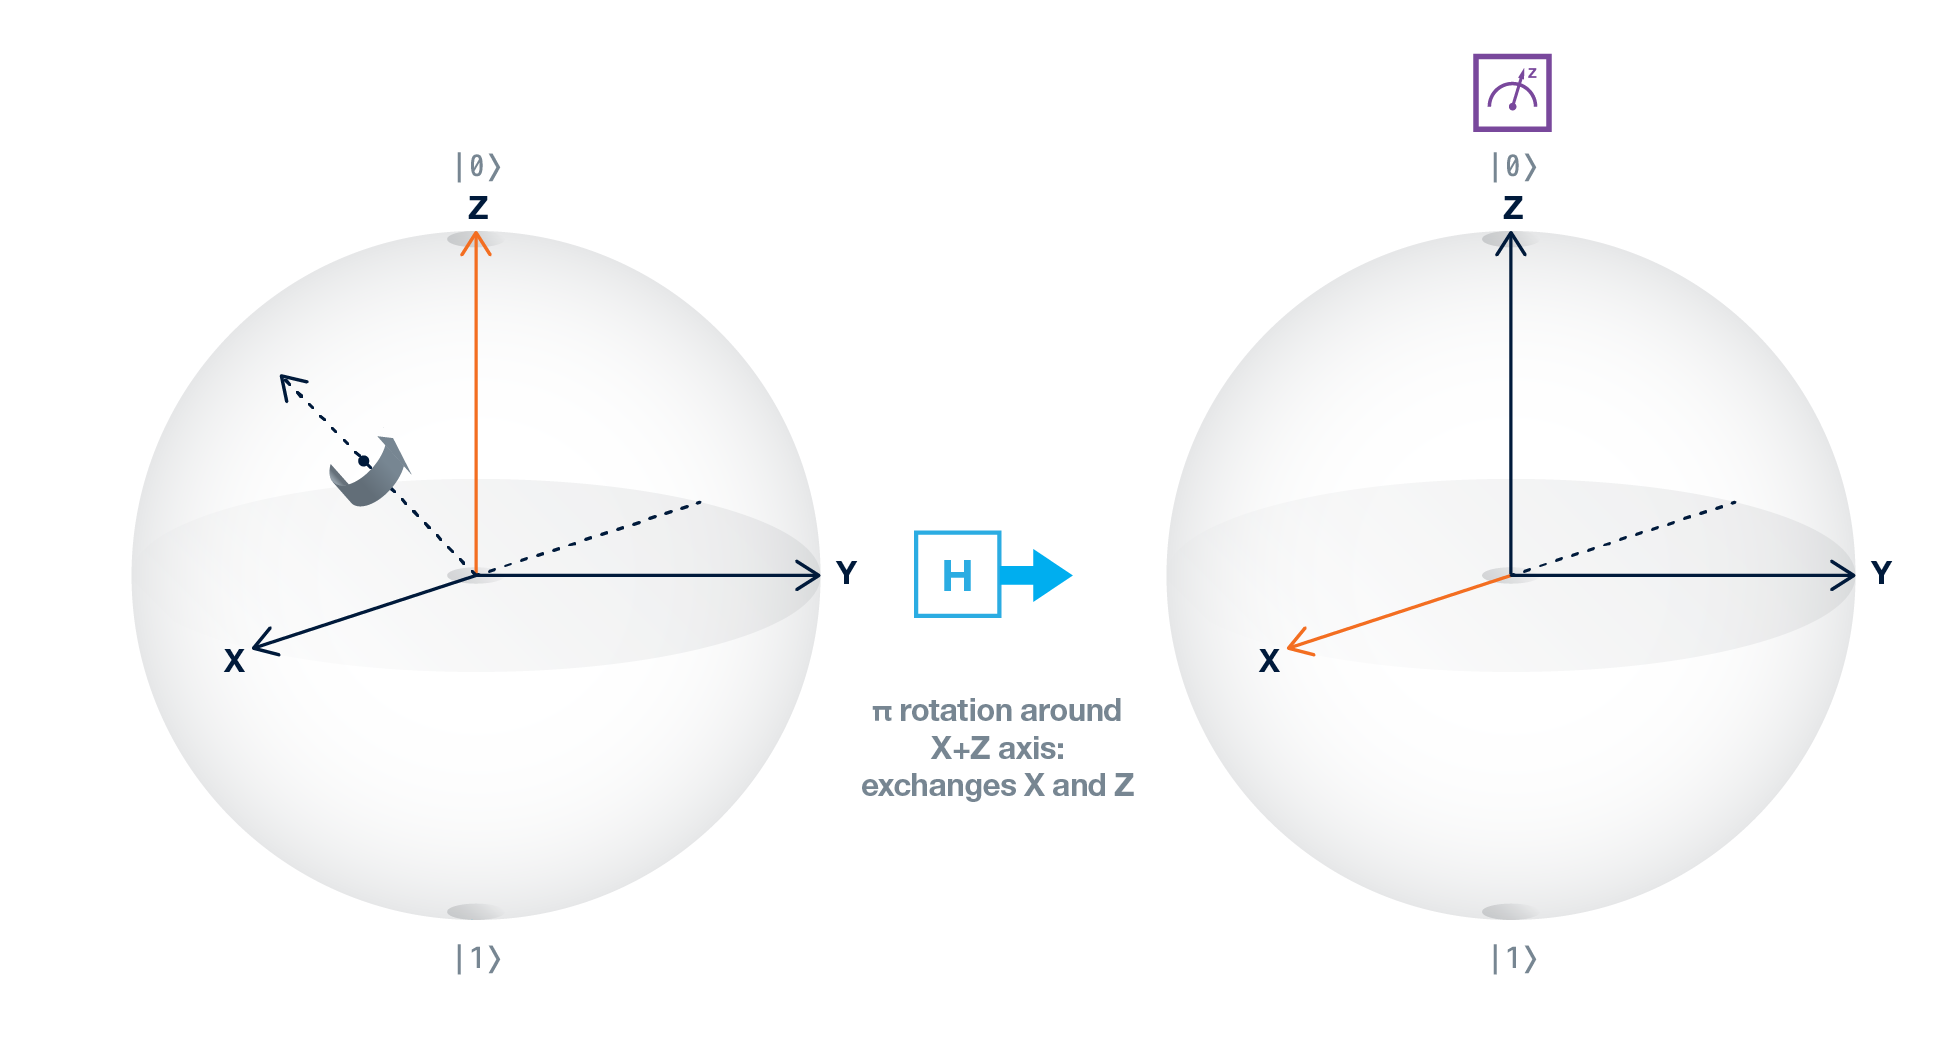
\includegraphics[width=.85\textwidth]{gate_h_bloch.png}
\end{frame}

\begin{frame}
    \frametitle{Quantum Gates}
    \begin{columns}
        \column{.4\textwidth}
            $\begin{array}{ccc}
                \textbf{Gate} & \textbf{Symbol} & \textbf{Unitary} \\
                \hline
                % Pauli X
                \text{Pauli X} & \Qcircuit @C=1.0em @R=0.0em @!R {
	         	    \lstick{} & \gate{X} & \qw \\
                } & \begin{bmatrix}
                    0 & 1 \\
                    1 & 0 \\
                \end{bmatrix} \\
                % Pauli Y
                \text{Pauli Y} & \Qcircuit @C=1.0em @R=0.0em @!R {
	         	    \lstick{} & \gate{Y} & \qw \\
                } & \begin{bmatrix}
                    0 & -i \\
                    i & 0 \\
                \end{bmatrix} \\
                % Pauli Z
                \text{Pauli Z} & \Qcircuit @C=1.0em @R=0.0em @!R {
	         	    \lstick{} & \gate{Z} & \qw \\
                } & \begin{bmatrix}
                    1 & 0 \\
                    0 & -1 \\
                \end{bmatrix} \\
                % hadamard
                \text{Hadamard} & \Qcircuit @C=1.0em @R=0.0em @!R {
	         	    \lstick{} & \gate{H} & \qw \\
                } & \frac{1}{\sqrt{2}}\begin{bmatrix}
                    1 & 1 \\
                    1 & -1 \\
                \end{bmatrix} \\
                % CX
                \text{CNOT} & \Qcircuit @C=1.0em @R=0.0em @!R {
                    \lstick{} & \ctrl{1} & \qw \\
                    \lstick{} & \targ & \qw \\
                } & \begin{bmatrix}
                    1 & 0 & 0 & 0 \\
                    0 & 0 & 0 & 1 \\
                    0 & 0 & 1 & 0 \\
                    0 & 1 & 0 & 0 \\
                \end{bmatrix} \\
            \end{array}$
        \column{.6\textwidth}
            \centering
            $\begin{array}{ccc}
                \textbf{Gate} & \textbf{Symbol} & \textbf{Unitary} \\
                \hline
                % U1
                \text{U1} & \Qcircuit @C=1.0em @R=0.0em @!R {
                    \lstick{} & \gate{U1(\lambda)} & \qw \\
                } & \begin{bmatrix}
                    1 & 0\\
                    0 & e^{i\lambda} \\
                \end{bmatrix} \\
                % U2
                \text{U2} & \Qcircuit @C=1.0em @R=0.0em @!R {
                    \lstick{} & \gate{U2(\phi,\lambda)} & \qw \\
                } & \frac{1}{\sqrt{2}} \begin{bmatrix}
                    1 & -e^{i\lambda} \\
                    e^{i\phi} & e^{i(\phi + \lambda} \\
                \end{bmatrix} \\
                % U3
                \text{U3} & \Qcircuit @C=1.0em @R=0.0em @!R {
                    \lstick{} & \gate{Rz(\phi)} & \qw \\
                } & U(\theta,\phi,\lambda) \\
                % Rz
                \text{Z Rotation} & \Qcircuit @C=1.0em @R=0.0em @!R {
                    \lstick{} & \gate{Rz(\phi)} & \qw \\
                } & \begin{bmatrix}
                    e^{-\frac{i\phi}{2}} & 0 \\
                    0 & e^{\frac{i\phi}{2}} \\
                \end{bmatrix} \\

                % SWAP
                \text{SWAP} & \Qcircuit @C=1.0em @R=0.0em @!R {
                    \lstick{} & \qswap & \qw\\
                    \lstick{} & \qswap \qwx[-1] & \qw\\
                } & \begin{bmatrix}
                    1 & 0 & 0 & 0 \\
                    0 & 0 & 1 & 0 \\
                    0 & 1 & 0 & 0 \\
                    0 & 0 & 0 & 1 \\
                \end{bmatrix}
            \end{array}$
    \end{columns}
\end{frame}

\subsubsection{OpenQASM}
\begin{frame}
    \frametitle{OpenQASM\footnotemark[1]\footnotemark[2]}
    \begin{columns}
        \column{0.5\textwidth}
            \lstinputlisting{bell.qasm}
        \column{0.5\textwidth}
            \begin{itemize}
                \item Open Quantum Assembly Language
                \item Can be used to write circuits
                \item Mostly used as a transport or to save circuits
            \end{itemize}
    \end{columns}
    \footnotetext[1]{\href{https://arxiv.org/abs/1707.03429}{https://arxiv.org/abs/1707.03429}}
    \footnotetext[2]{\href{https://github.com/Qiskit/openqasm}{https://github.com/Qiskit/openqasm}}
\end{frame}

\subsection{Pulse}
\begin{frame}
    \frametitle{Pulse Level Programming}
    \begin{columns}
        \column{0.5\textwidth}
            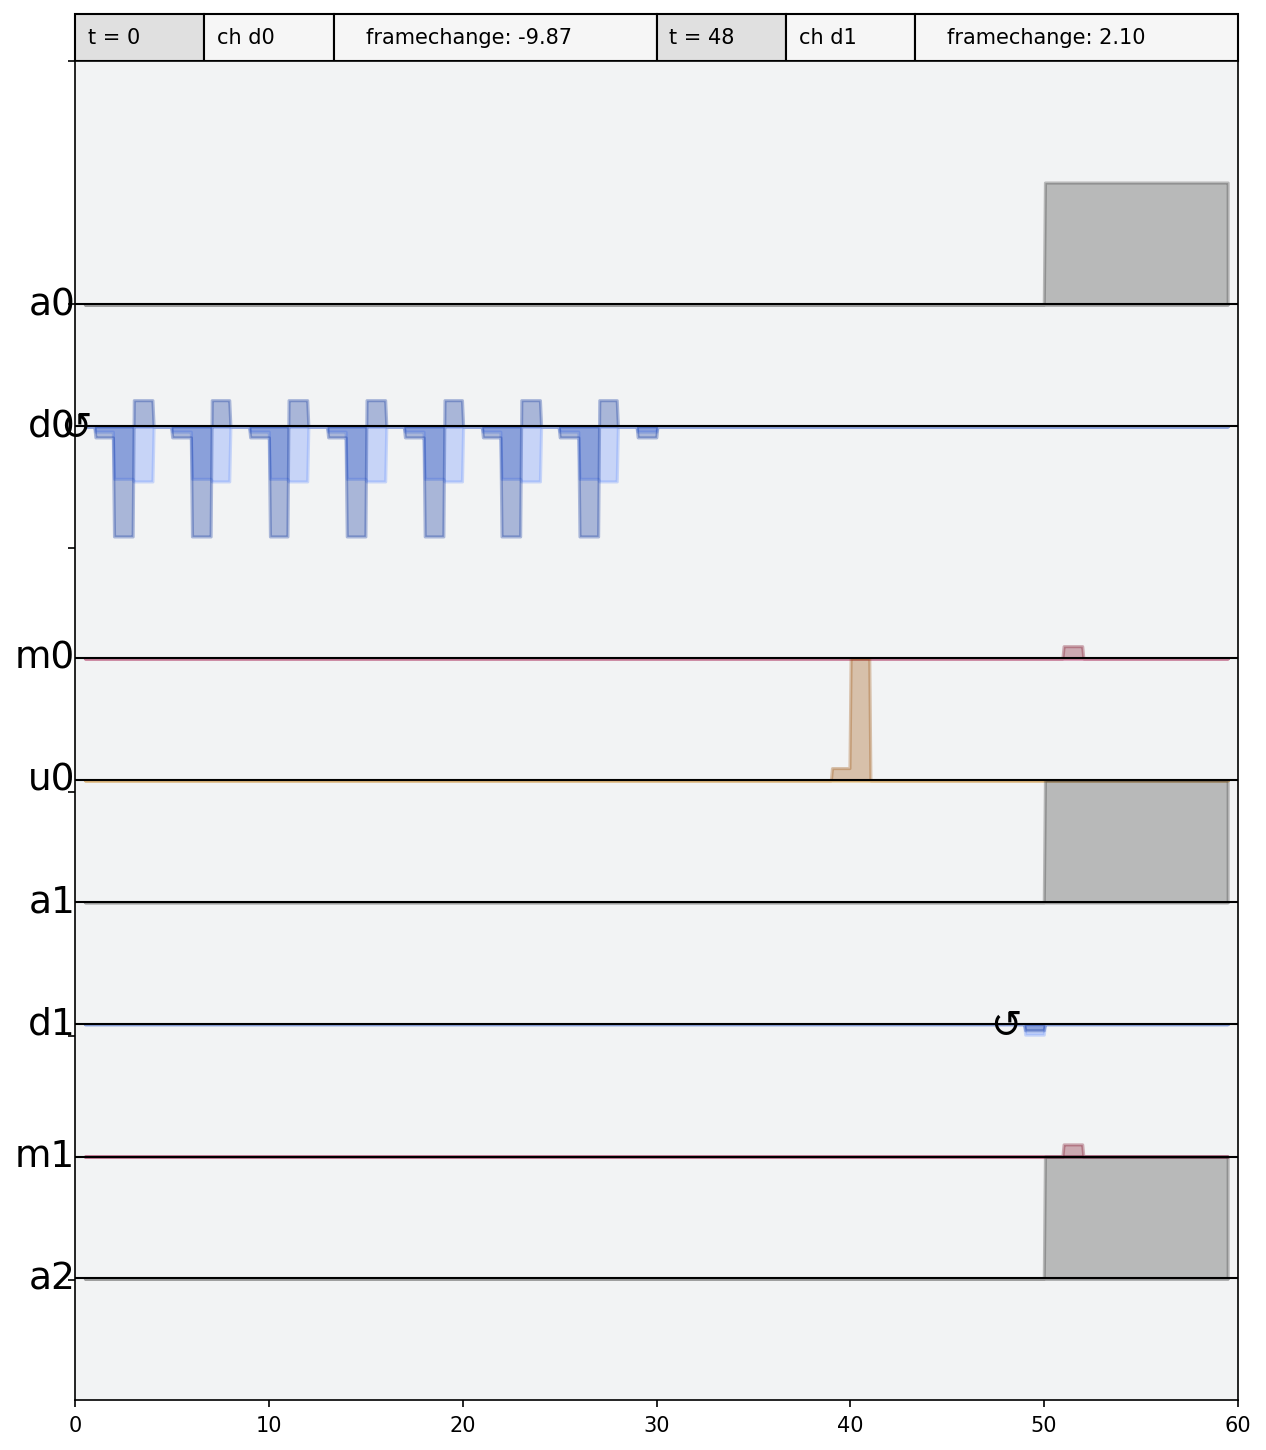
\includegraphics[width=\textwidth]{bell-sched.png}
        \column{0.5\textwidth}
            \begin{itemize}
                \item A layer below the circuit model is to use pulses
                \item Each quantum gate is defined as a pulse that gets
                    applied to the qubits
                \item Enables you to tweak the definition of gates
                \item Mostly used for physics research or hardware characterization
            \end{itemize}
    \end{columns}
\end{frame}

\section{Constraints for Running on Quantum Computers}
\begin{frame}
    \frametitle{Why do we need compilers?}
    \only<1>{
        \begin{itemize}
            \item Despite programming at a low (per bit) level it still is abstracted from the hardware.
            \item The compiler is used to enable running logical abstract circuit
                on an actual device
            \item NISQ devices have a number of limitations
        \end{itemize}
        \centering
        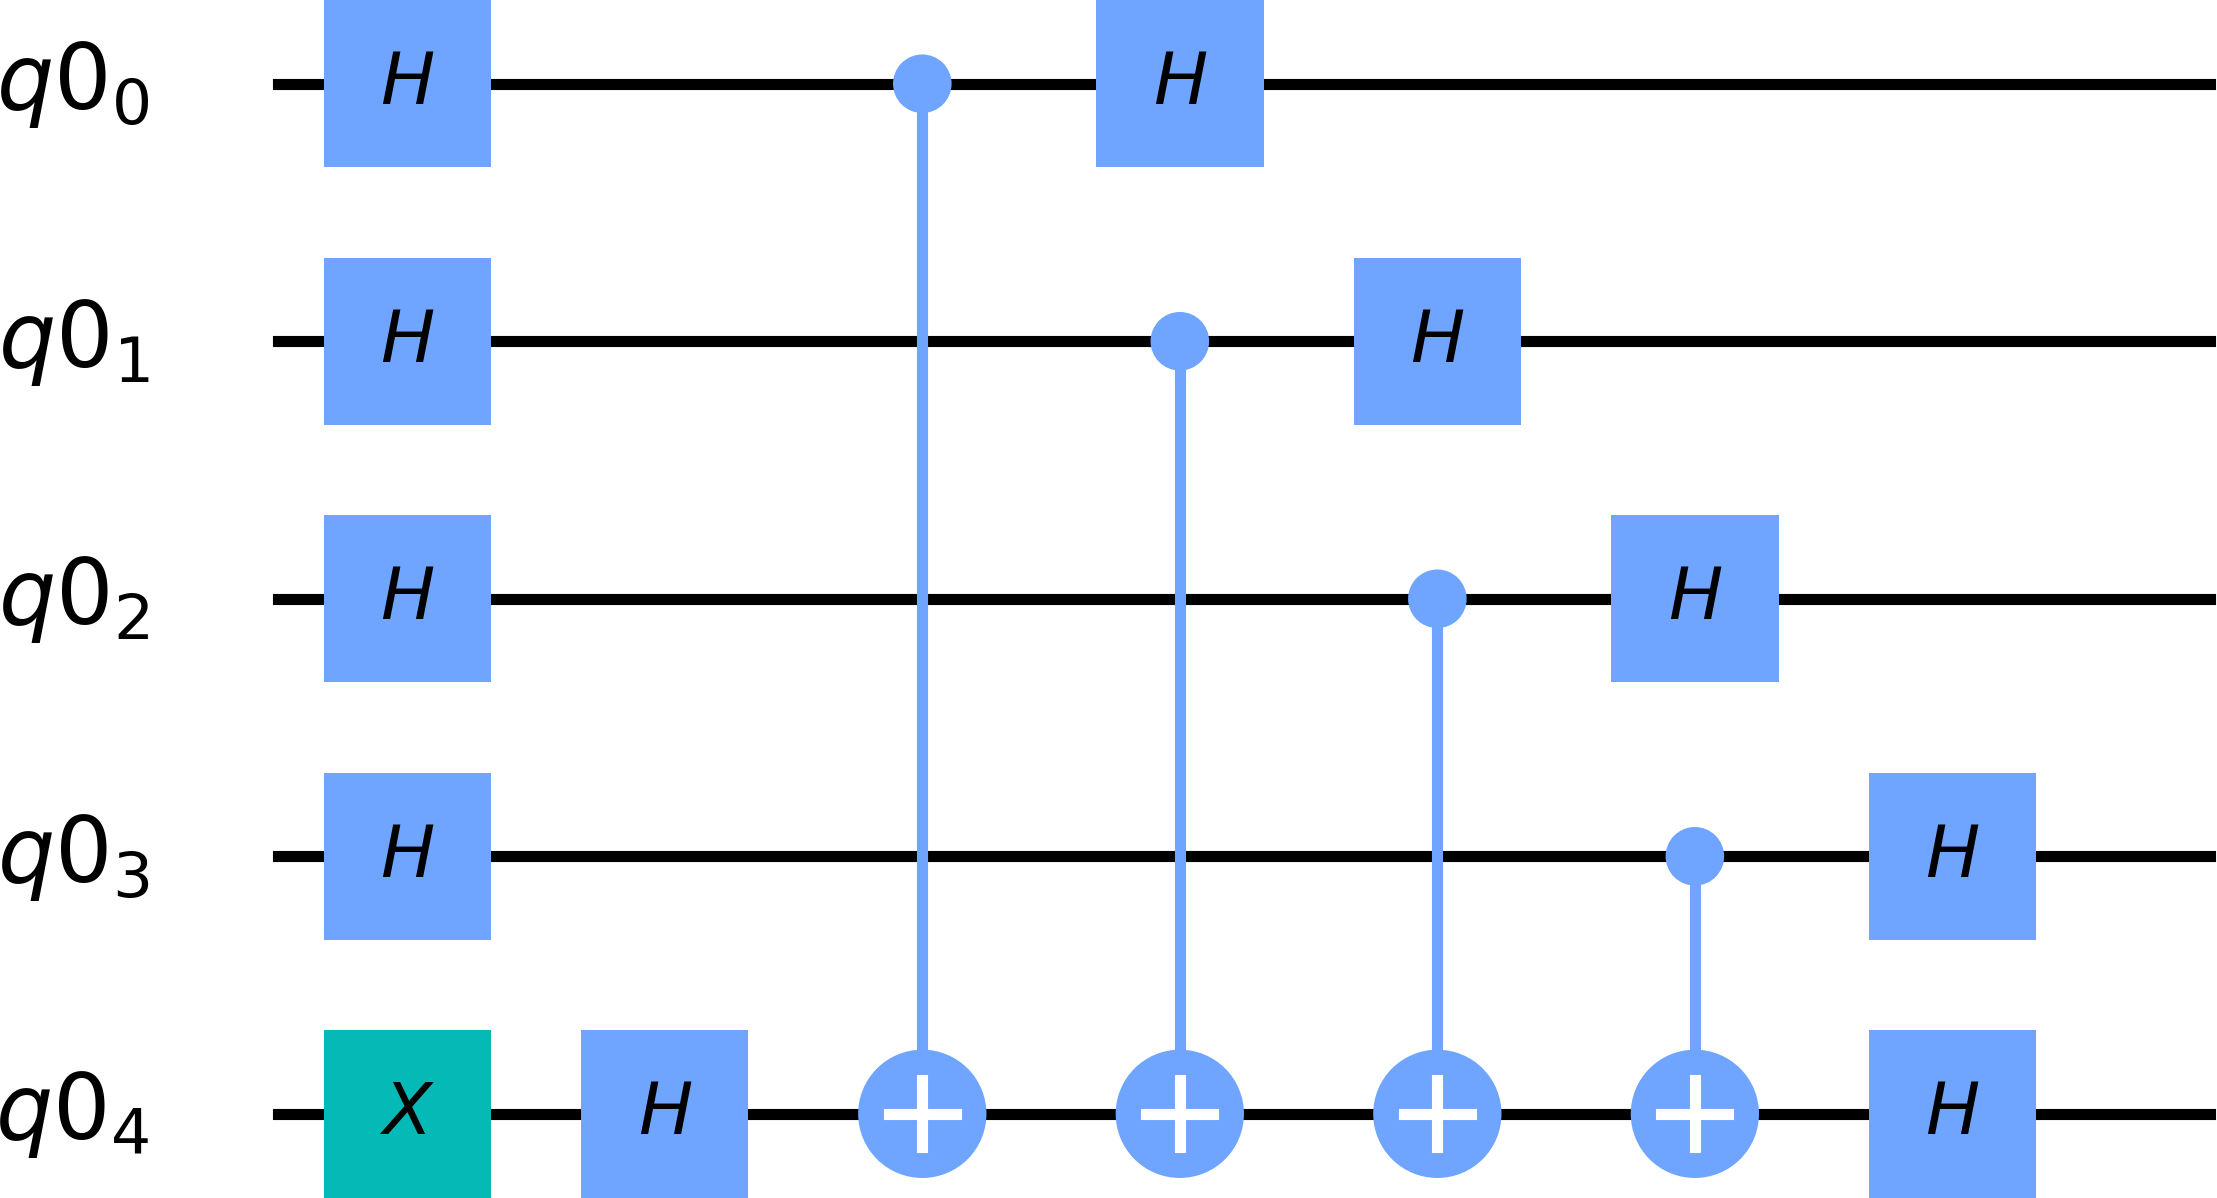
\includegraphics[width=\textwidth,height=.6\textheight,keepaspectratio]{no_compile.png}
    }
    \only<2>{
            \centering
            \textbf{Bad Compilation}
            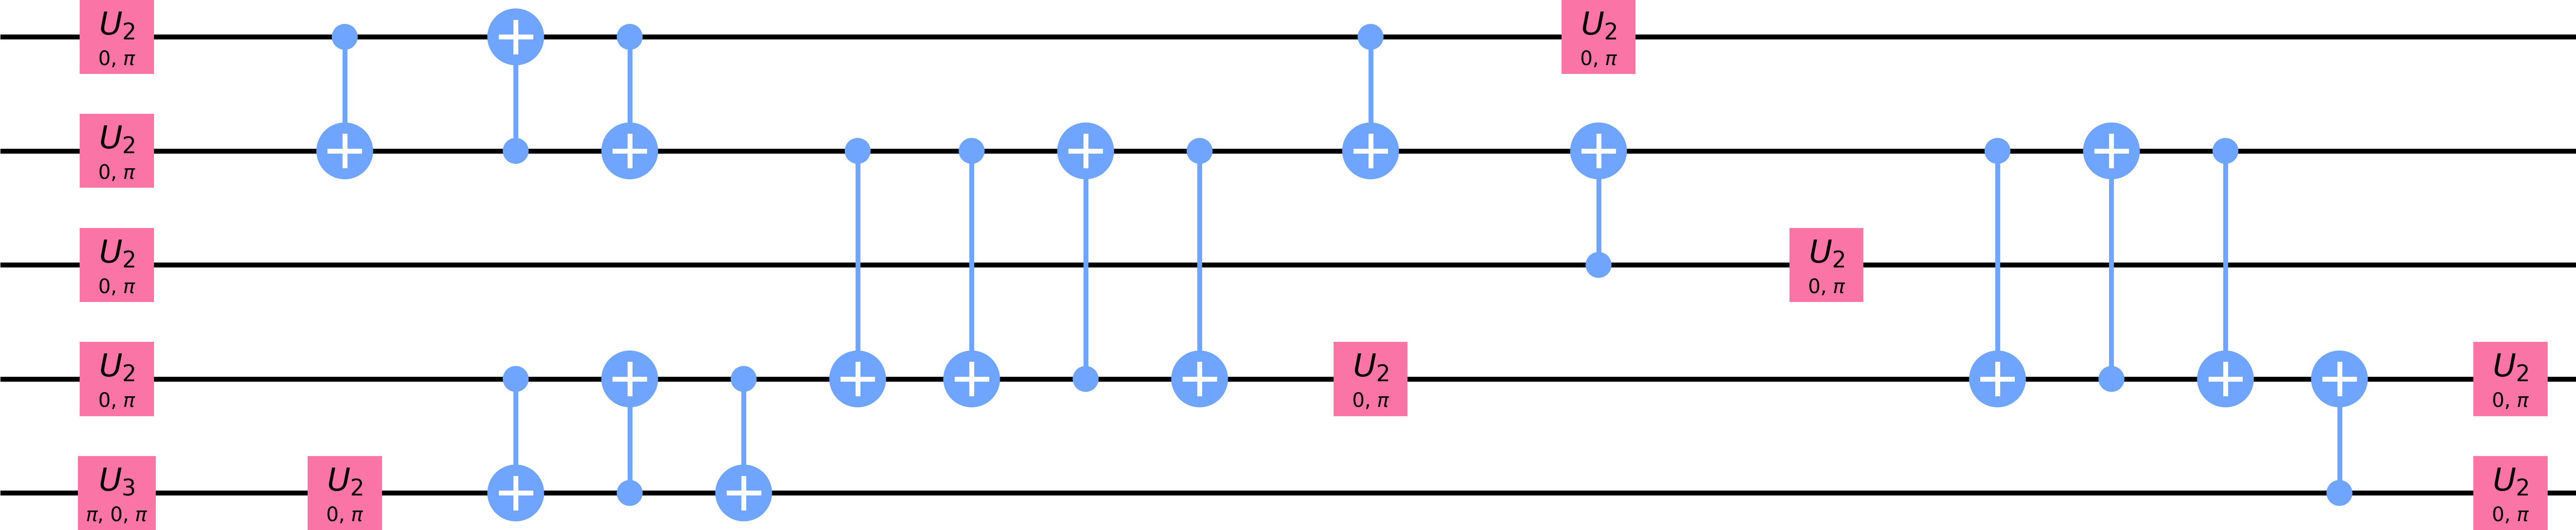
\includegraphics[width=\textwidth]{bad_compile_circ.png}
            \centering
            \textbf{Good Compilation}
            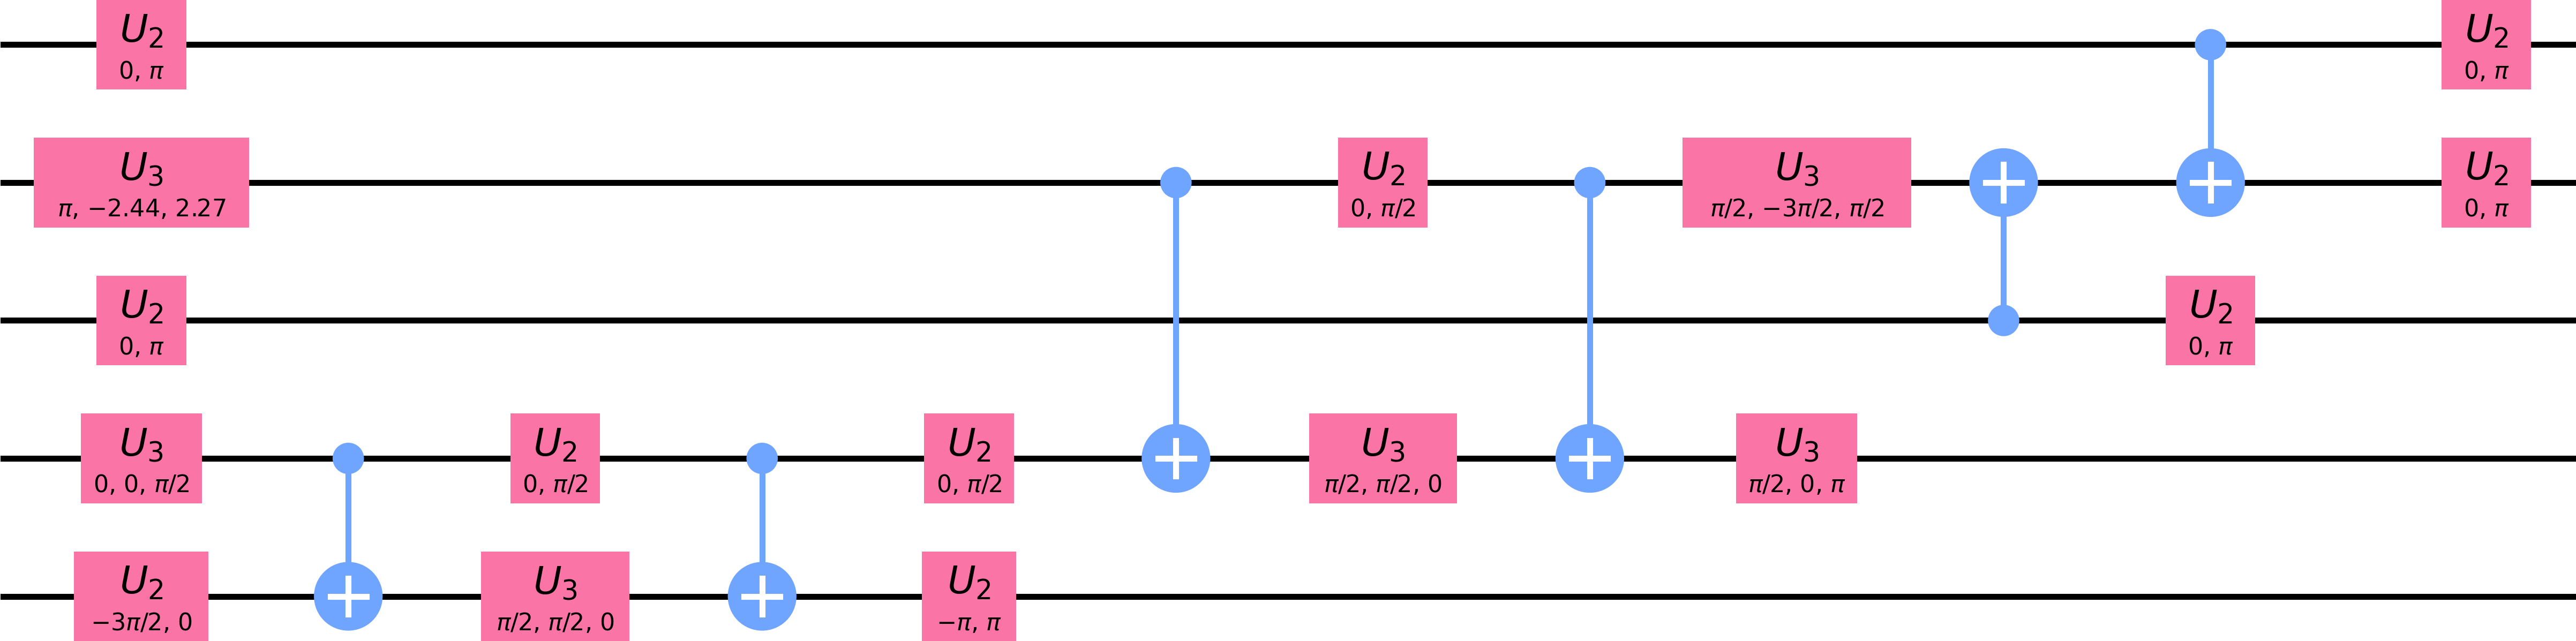
\includegraphics[width=\textwidth]{good_compile_circ.png}
    }
    \only<3>{
        \begin{columns}
            \column{.45\textwidth}
                \centering
                \textbf{Bad Compilation}
                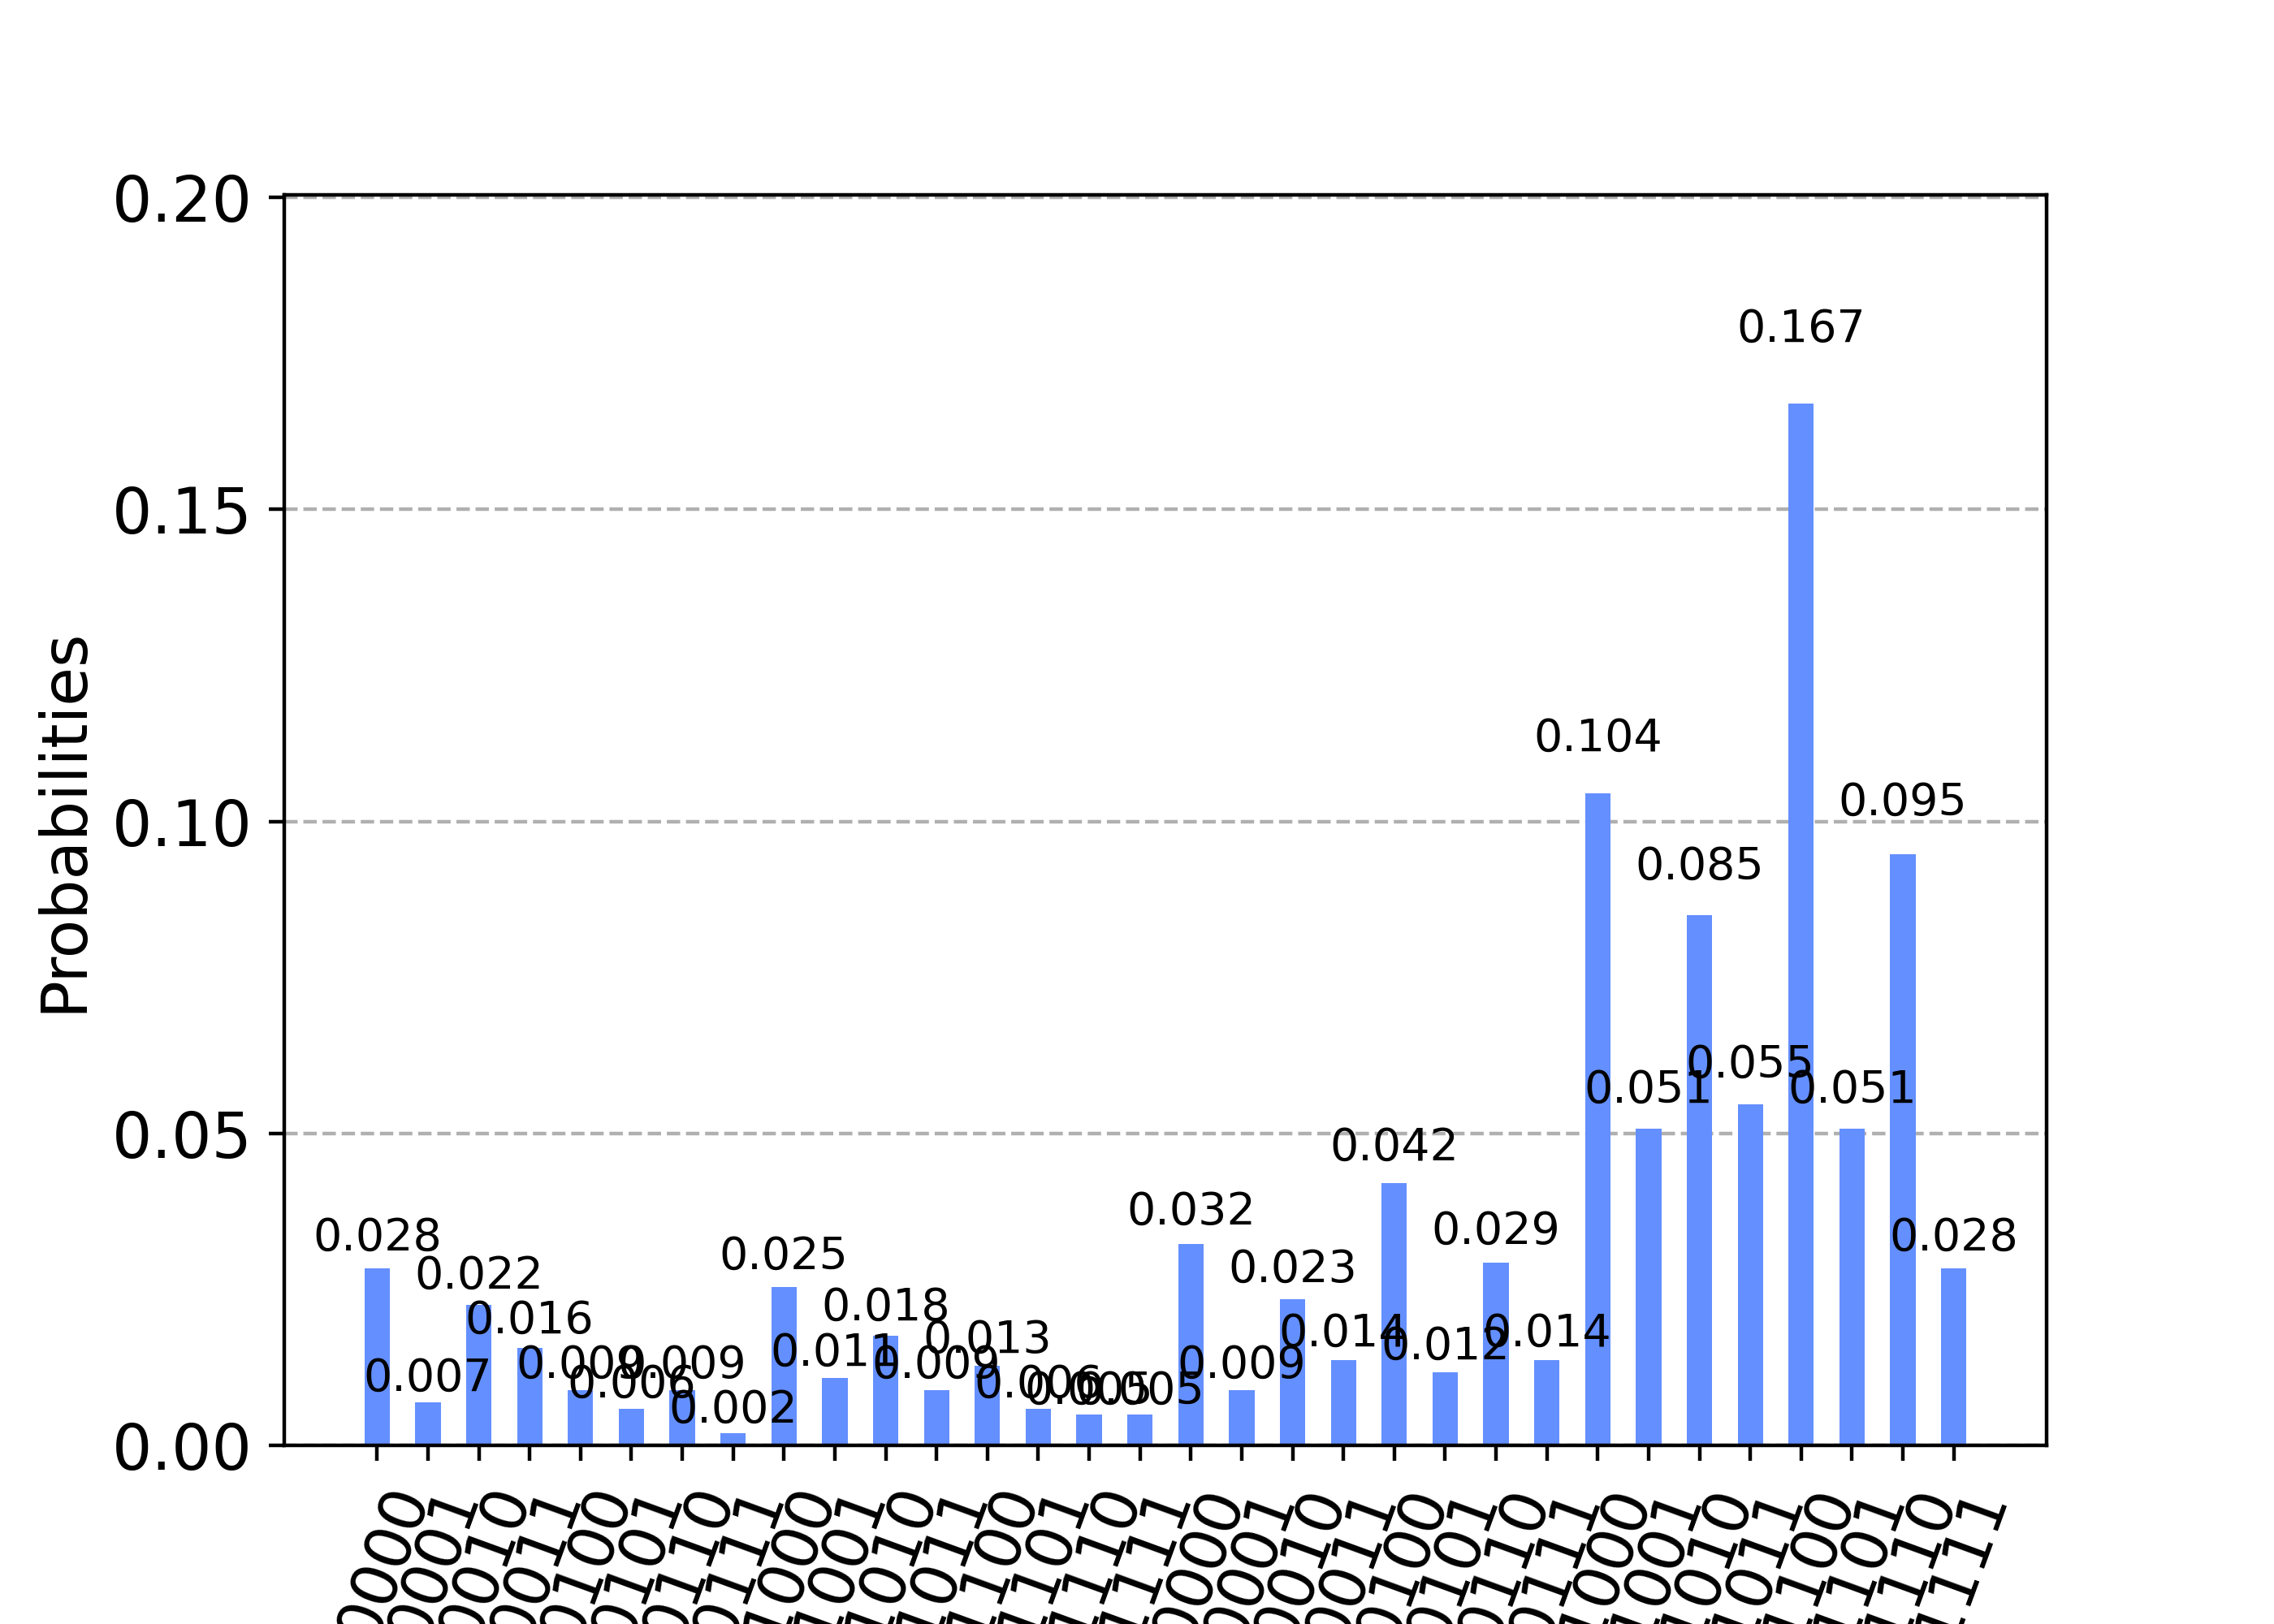
\includegraphics[width=\textwidth]{bad_compile.png}
            \column{.45\textwidth}
                \centering
                \textbf{Good Compilation}
                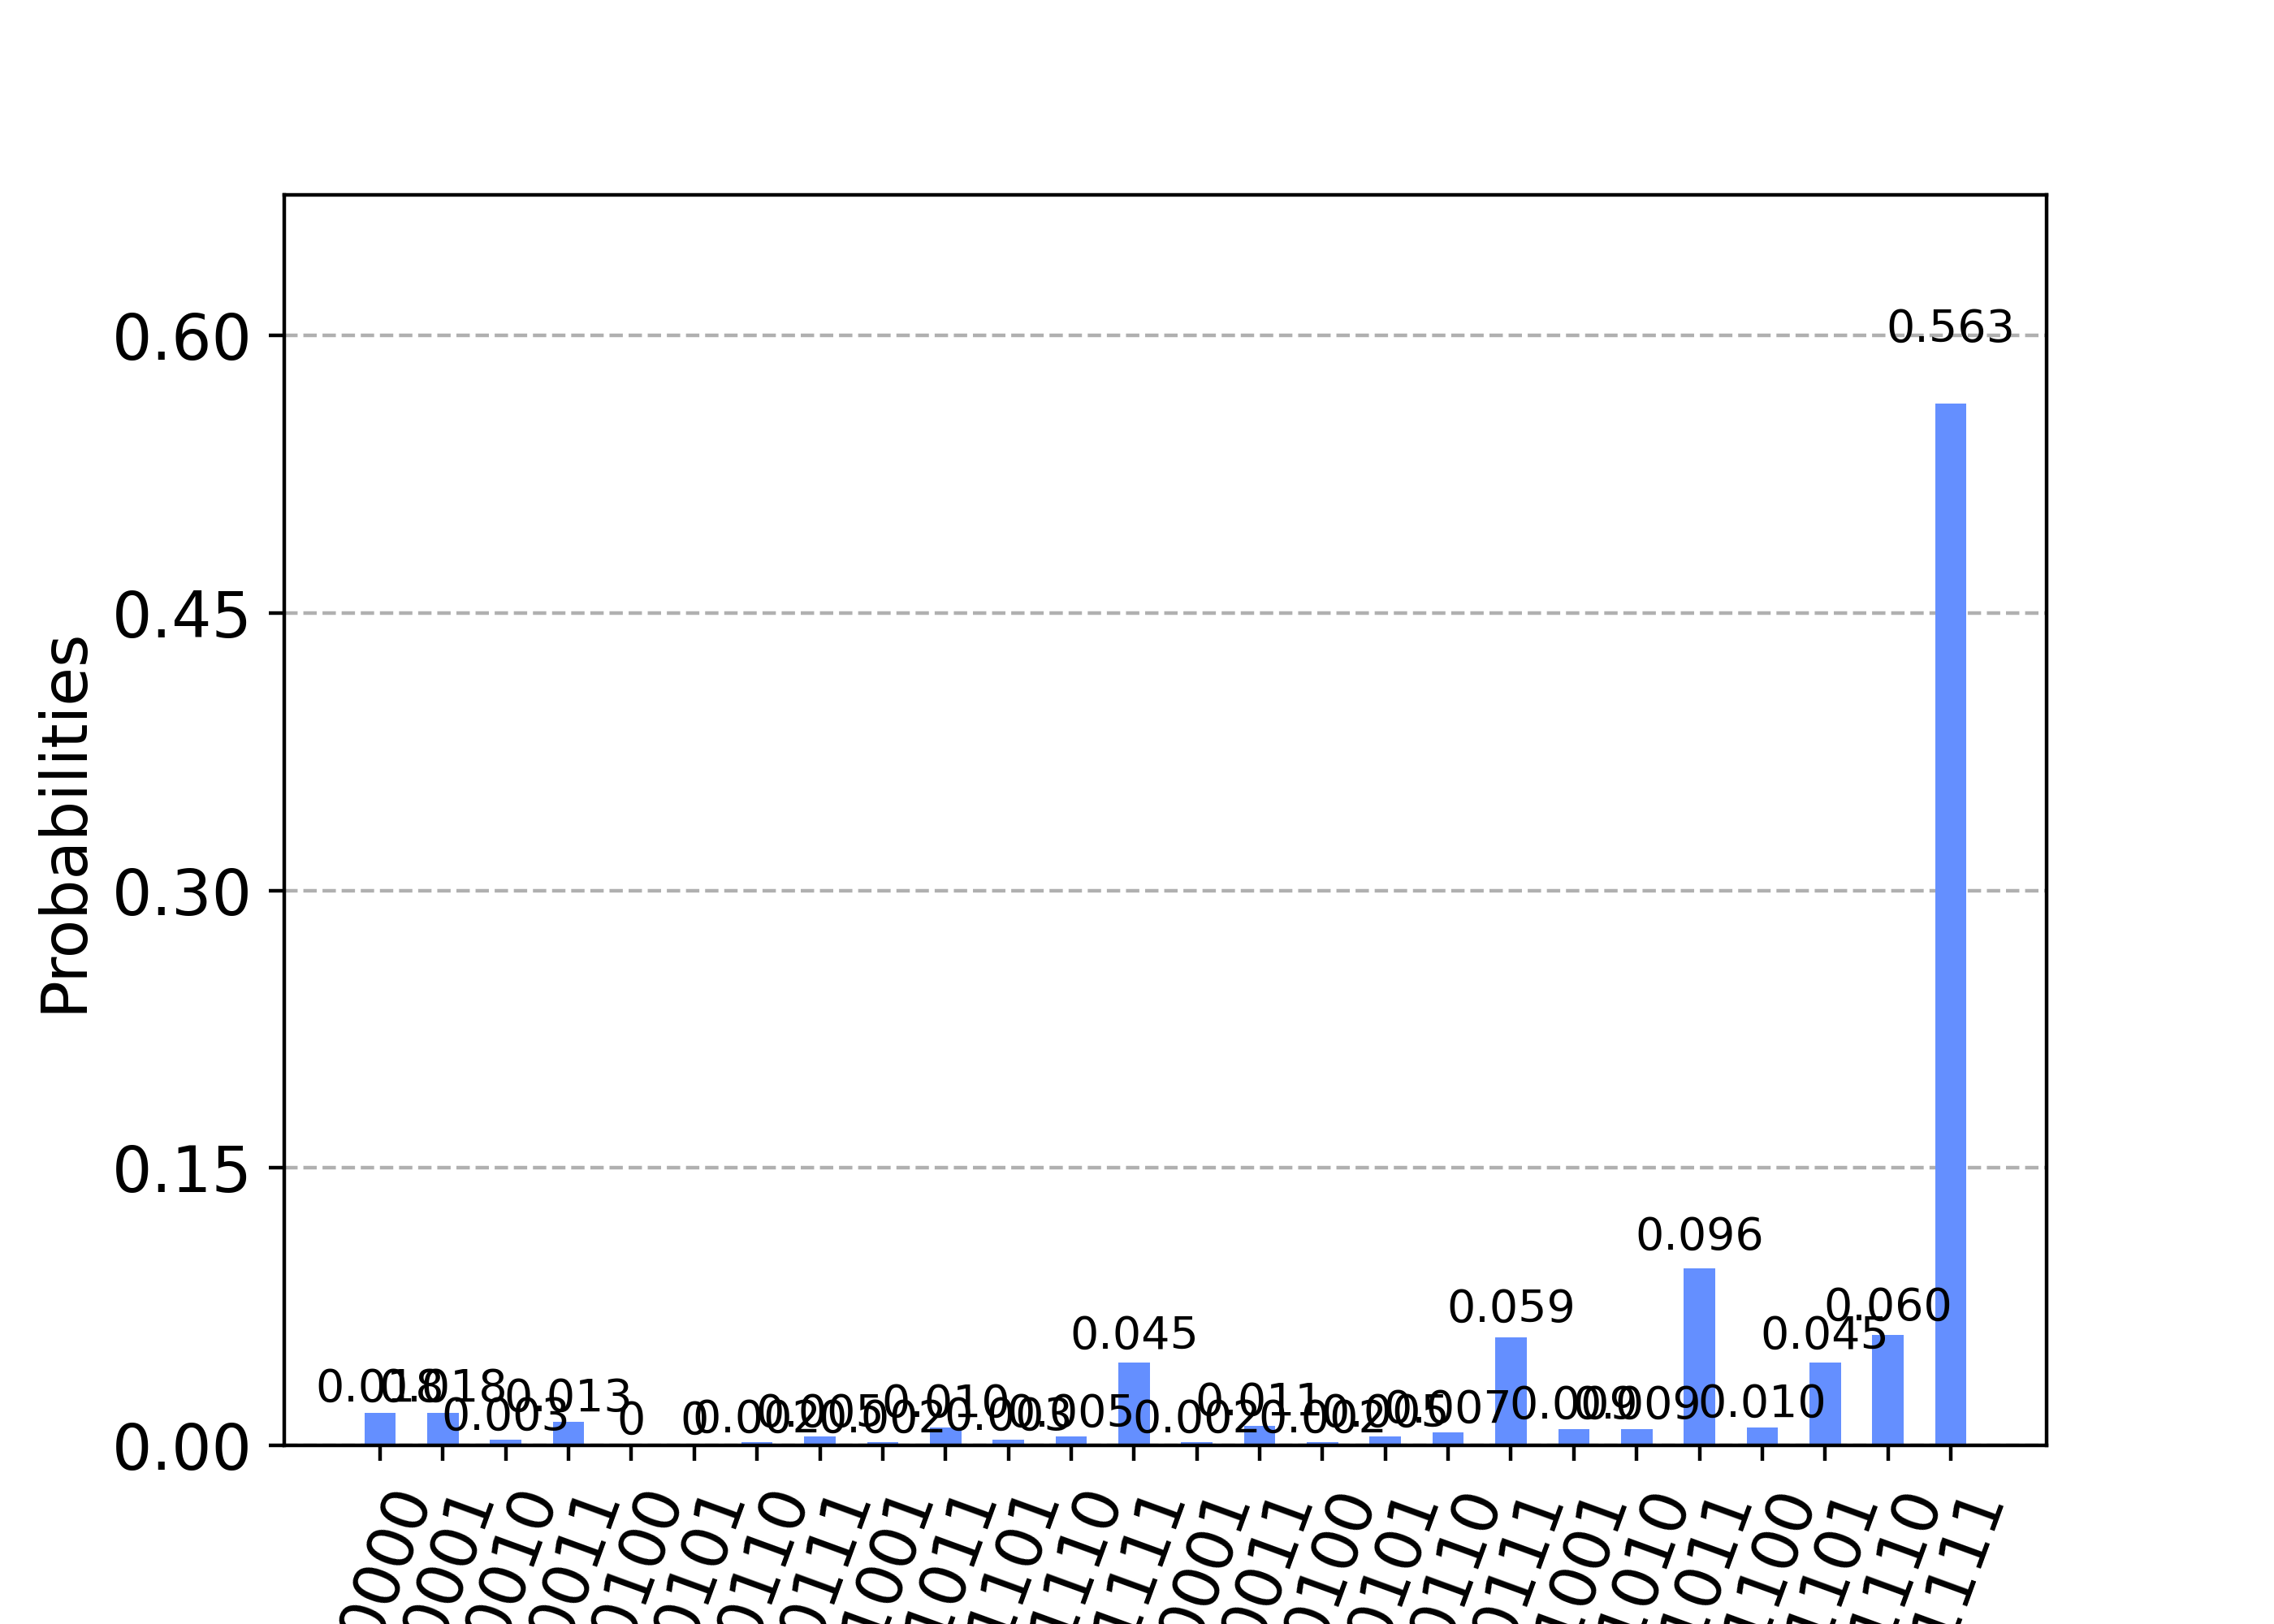
\includegraphics[width=\textwidth]{good_compile.png}
         \end{columns}
    }
\end{frame}

\subsection{Device Characteristics}
\begin{frame}
    \frametitle{Basis Gates}
    \begin{columns}
        \column{.5\textwidth}
        \begin{itemize}
            \item Each Quantum Computer only supports a small set of basis gates
            \item These gates can be used to implement any other
            \item For circuits to be executable by a quantum computer they
                must be expressed in terms of their basis gates
        \end{itemize}
        \column{.5\textwidth}
            \textbf{Superconducting Qubits:}\\
                Cx, U3, id\\
            \textbf{Trapped Ion Qubits:}\\
                Ms, Rx, Ry\\
            \textbf{Simulator:}\\
                U1, U2, U3, Cx, Cz, Id, X, Y, Z, H, S, Sdg, t, tdg, swap, ccx, unitary, initialize, cu1, cu2, cu3, swap, mcx, mcz, mcu1, mcu2, mcu3, mcswap, muliplexer\\
    \end{columns}
\end{frame}

\subsection{Qubit Connectivity}
\begin{frame}
    \frametitle{Qubit Connectivity}
    \begin{columns}
        \column{.5\textwidth}
            \begin{itemize}
                \item Qubits in a device have limited connectivity
                \item For multi-qubit gates this means we can only run them
                    between those qubits
            \end{itemize}
        \column{.5\textwidth}
            \centering
            \only<1>{\textbf{IBM Q 5 Yorktown}\\}
            \only<1>{\includegraphics[width=\textwidth]{ibmqx2-labeled.png}}
            \only<2>{\textbf{IBM Q 53 Rochester Coupling Map}\\}
            \only<2>{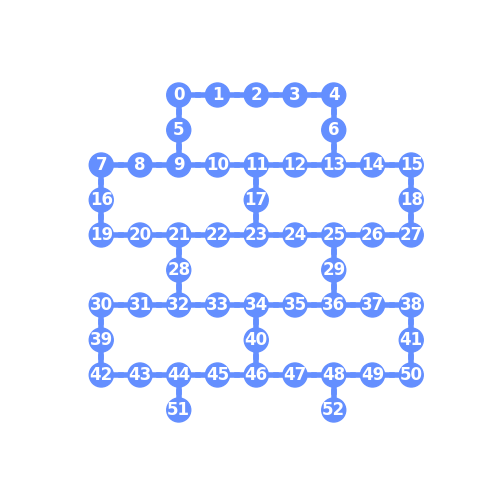
\includegraphics[width=\textwidth]{rochester_map.png}}
    \end{columns}
\end{frame}

\begin{frame}
    \frametitle{Not Enough Connectivity}
    \begin{columns}
        \column{.5\textwidth}
            \begin{itemize}
                \item If there
                \item Use SWAP gate to move state around
            \end{itemize}
        \column{.5\textwidth}
            \textbf{SWAP Gate}
            \begin{equation*}
                \Qcircuit @C=1.0em @R=1.0em @!R {
	 	            \lstick{ {q}_{0} : \ket{0} } & \qswap & \qw & \qw\\
            	    \lstick{ {q}_{1} : \ket{0} } & \qswap \qwx[-1] & \qw & \qw\\
            	}
            \end{equation*}
            $\equiv$
            \begin{equation*}
                \Qcircuit @C=1.0em @R=0.2em @!R {
            	 	\lstick{ {q}_{0} : \ket{0} } & \ctrl{1} & \targ & \ctrl{1} & \qw & \qw\\
	         	    \lstick{ {q}_{1} : \ket{0} } & \targ & \ctrl{-1} & \targ & \qw & \qw\\
                }
            \end{equation*}
    \end{columns}
\end{frame}

\subsection{Noise}
\begin{frame}
    \frametitle{Noise}
    \begin{columns}
        \column{.5\textwidth}
            \begin{itemize}
                \item Gate Errors
                    \begin{itemize}
                        \item Single Qubit Errors
                        \item Multiqubit Errors
                    \end{itemize}
                \item Decoherence
                    \begin{itemize}
                        \item T1: Energy relaxation, the time for a qubit at
                            $\ket{1}$ to decay to ground state $\ket{0}$
                        \item T2: dephasing of a qubit in superposition state
                    \end{itemize}
                \item Readout Error
            \end{itemize}
        \column{.5\textwidth}
            \only<1>{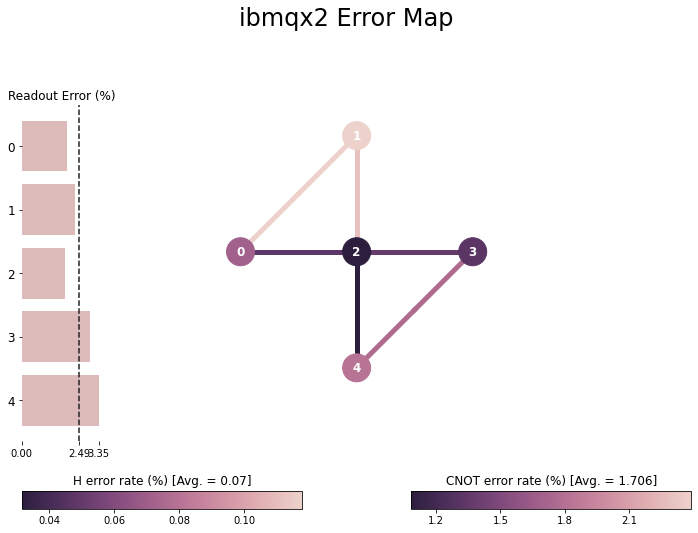
\includegraphics[width=\textwidth]{error_map.png}}
            \only<2>{
                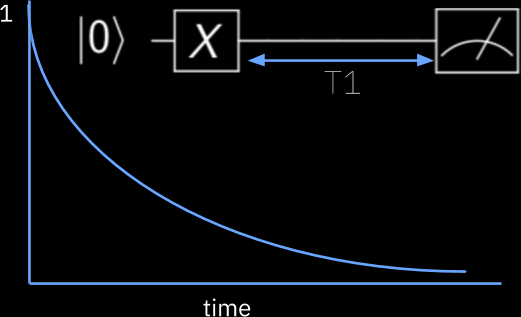
\includegraphics[width=\textwidth]{decoherence_t1.png}
                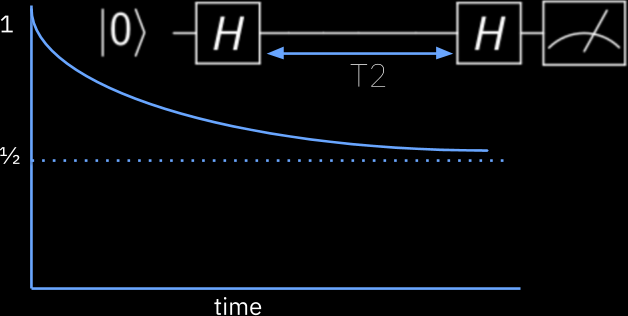
\includegraphics[width=\textwidth]{decoherence_t2.png}
            }
    \end{columns}
\end{frame}

\section{Qiskit's Compiler}
\begin{frame}
    \frametitle{Qiskit Terra\footnotemark[1]}
    \begin{columns}
          \column{.5\textwidth}
             \begin{itemize}
                  \item Is the base layer for working with quantum computers provides interface to hardware and simulators
                  \item Provides an SDK for working with quantum circuits
                  \item Compiles circuits to run on different backends
                  \item Designed to be backend agnostic and work with any
                      quantum hardware or simulator
                  \item Written in Python
                  \item Apache 2.0 Licensed
             \end{itemize}
          \column{.5\textwidth}
              \centering
              \colorbox{black}{
\includegraphics[width=.5\textwidth]{qiskit-terra-logo.png}}
      \end{columns}
      \footnotetext[1]{\href{https://github.com/Qiskit/qiskit-terra}{https://github.com/Qiskit/qiskit-terra}}
  \end{frame}

\subsection{The DAG}
\begin{frame}
    \frametitle{The DAG}
        \begin{columns}
            \column{0.45\textwidth}
                \begin{itemize}
                    \item Compiler represents circuits as a DAG
                    \item Each node in the DAG is an operation, an input, or
                          an output
                    \item Each edge indicates data flow between nodes
                    \item Makes flow of information between operations
                        explicit
                \end{itemize}
            \column{0.45\textwidth}
                \centering
                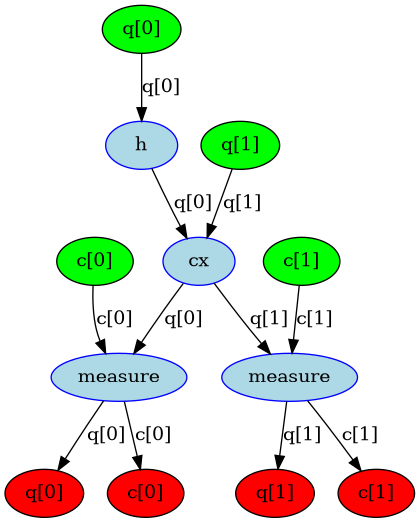
\includegraphics[width=0.75\textwidth]{bell-dag.png}
        \end{columns}
\end{frame}

\begin{frame}
    \frametitle{The DAG}
    \begin{columns}
        \column{0.45\textwidth}
            \centering
            \begin{equation*}
                \Qcircuit @C=1.0em @R=0.0em @!R {
            	 	\lstick{ {q}_{0} : \ket{0} } & \gate{H} & \ctrl{1} & \meter & \qw & \qw & \qw\\
                	\lstick{ {q}_{1} : \ket{0} } & \qw & \targ & \qw & \gate{R_z(0.5)} & \qw & \qw\\
                	\lstick{ {q}_{2} : \ket{0} } & \qw & \qw & \qw & \qw & \qw & \qw\\
                	\lstick{c_{0}: 0} & \cw & \cw & \cw \cwx[-3] & \controlo \cw \cwx[-2] & \cw & \cw\\
                	\lstick{c_{1}: 0} & \cw & \cw & \cw & \control \cw \cwx[-1] & \cw & \cw\\
                	\lstick{c_{2}: 0} & \cw & \cw & \cw & \controlo \cw \cwx[-1] & \cw & \cw\\
                }
            \end{equation*}
        \column{.01\textwidth}
            \centering
            $\rightarrow$
        \column{0.45\textwidth}
            \centering
            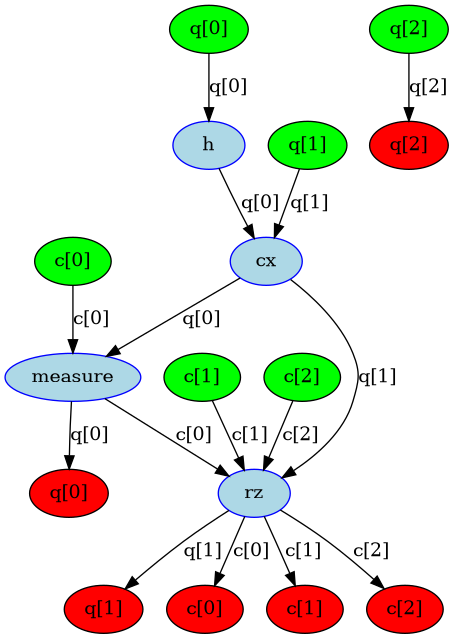
\includegraphics[width=0.75\textwidth]{classical_dep_dag.png}
        \end{columns}
\end{frame}
{
\setbeamercolor{background canvas}{bg=black}
\setbeamercolor{footline}{fg=ibm}
\begin{frame}
    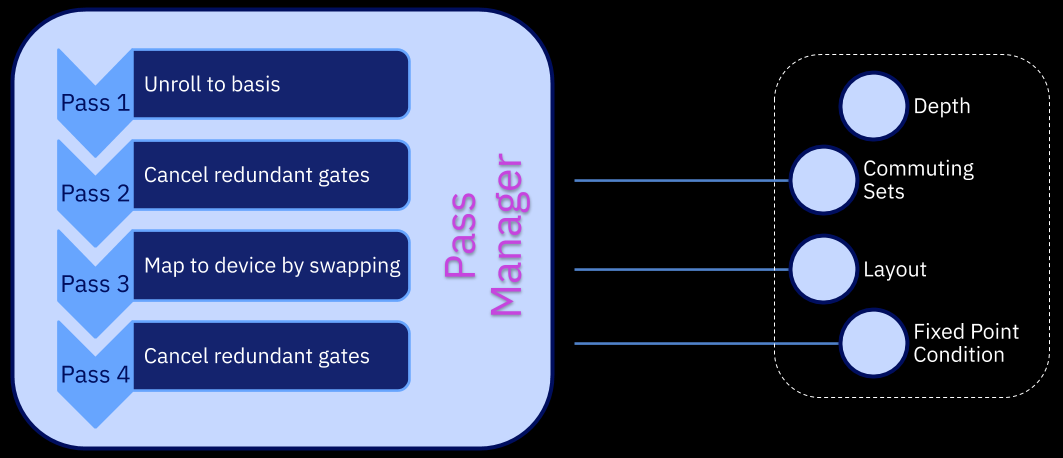
\includegraphics[width=\textwidth]{passmanager.png}
\end{frame}

\begin{frame}
    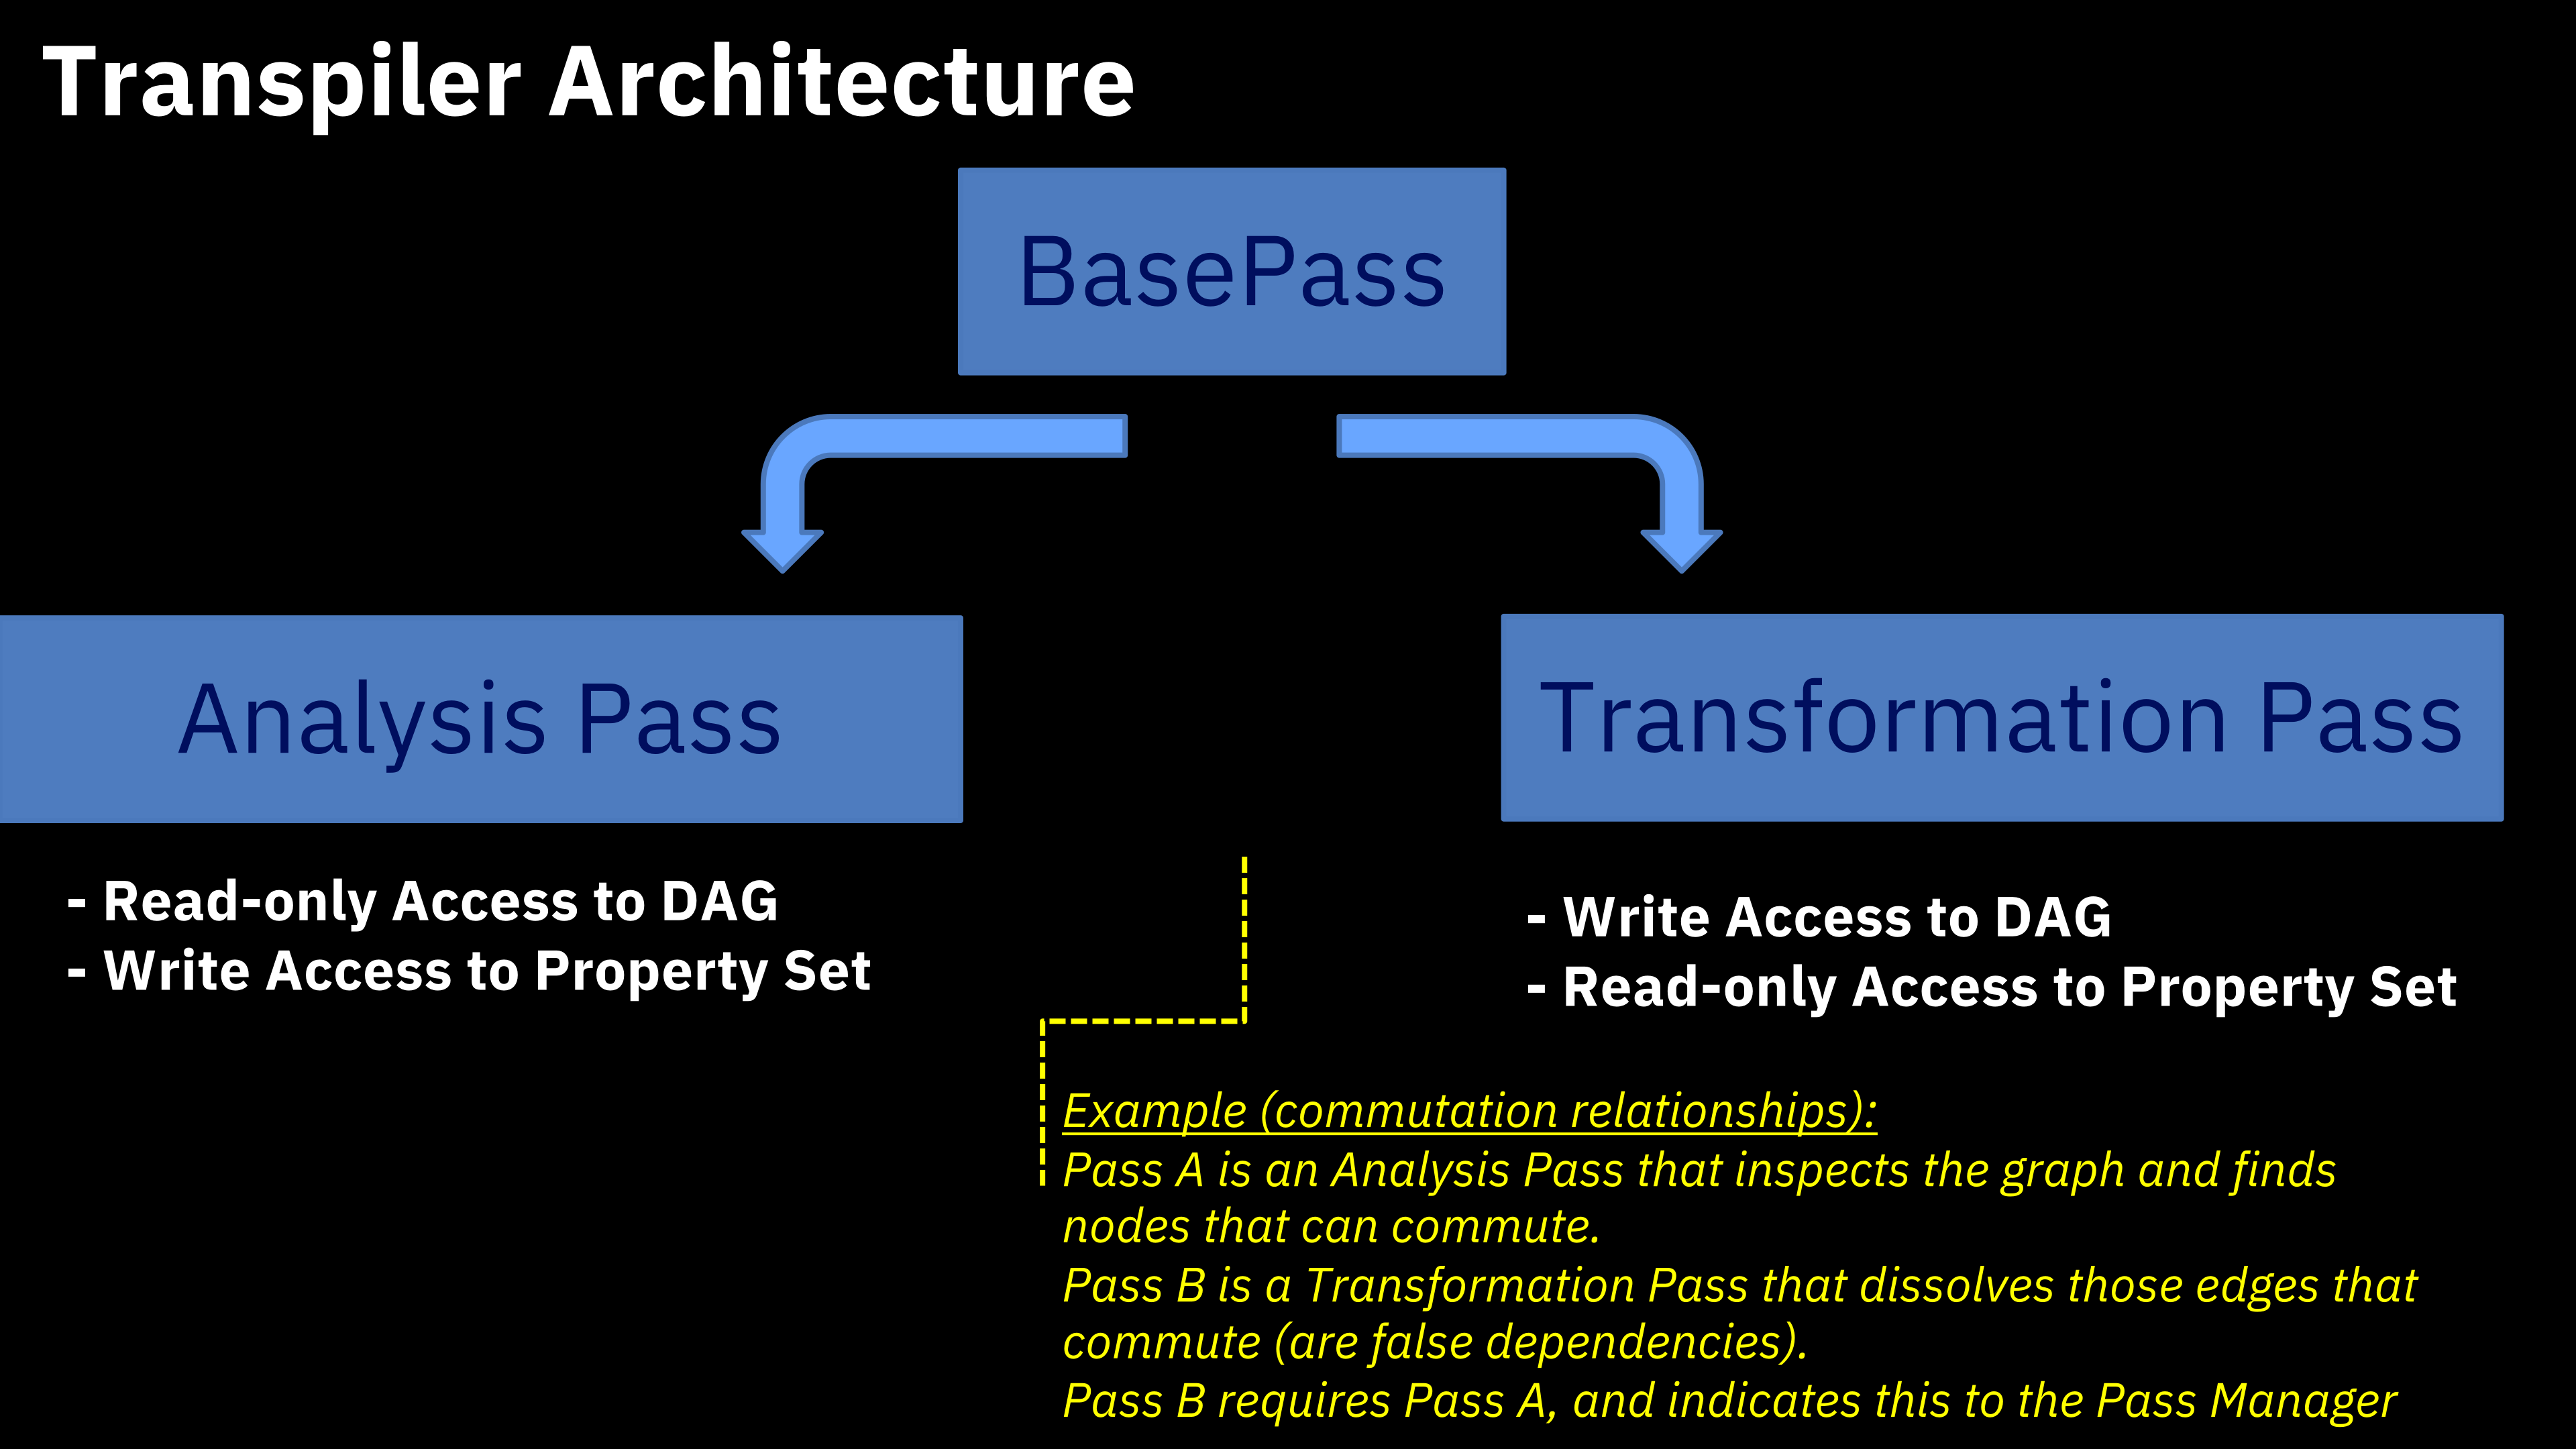
\includegraphics[width=\textwidth]{passmanager_2.png}
\end{frame}
}
\begin{frame}
    \frametitle{Passmanager Stages}
    \begin{columns}
        \column{.45\textwidth}
            \begin{itemize}
                \item Stages
                    \begin{itemize}
                        \item Logical Reductions
                        \item Embedding
                            \begin{itemize}
                                \item Layout
                                \item Mapping/Routing
                                \item Unrolling
                            \end{itemize}
                        \item Physical Reductions
                    \end{itemize}
                \item Pluggable and extensible
            \end{itemize}
        \column{.45\textwidth}
            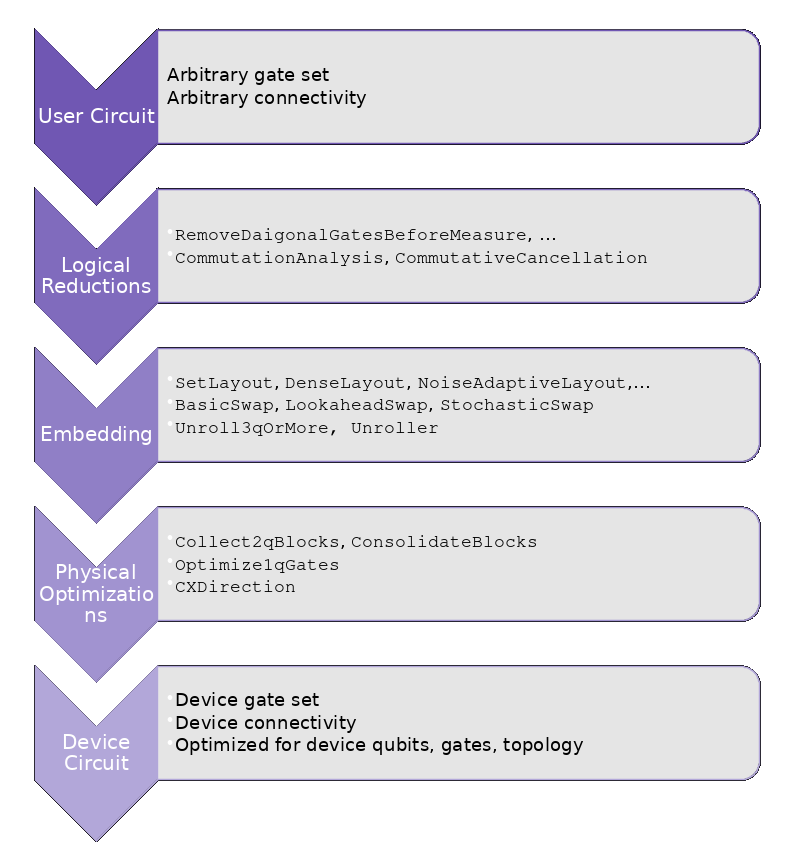
\includegraphics[width=\textwidth]{passmanager_stages.png}
    \end{columns}
\end{frame}
\subsection{Preset Pass Managers}
\begin{frame}
    \frametitle{Preset Pass Managers}
    \begin{itemize}
        \item Out of the box 4 optimization levels (0-3) with preset pass managers
        \item Increasing levels of optimization vs execute time
    \end{itemize}
\end{frame}
\begin{frame}
    \centering
    \only<1>{
    \textbf{Optimization Level 0}\\
    \begin{columns}
        \column{.5\textwidth}
        \begin{itemize}
            \item No Optimization
            \item Unroll
            \item Trivial Layout
            \item Swap Mapping
        \end{itemize}
        \column{.5\textwidth}
        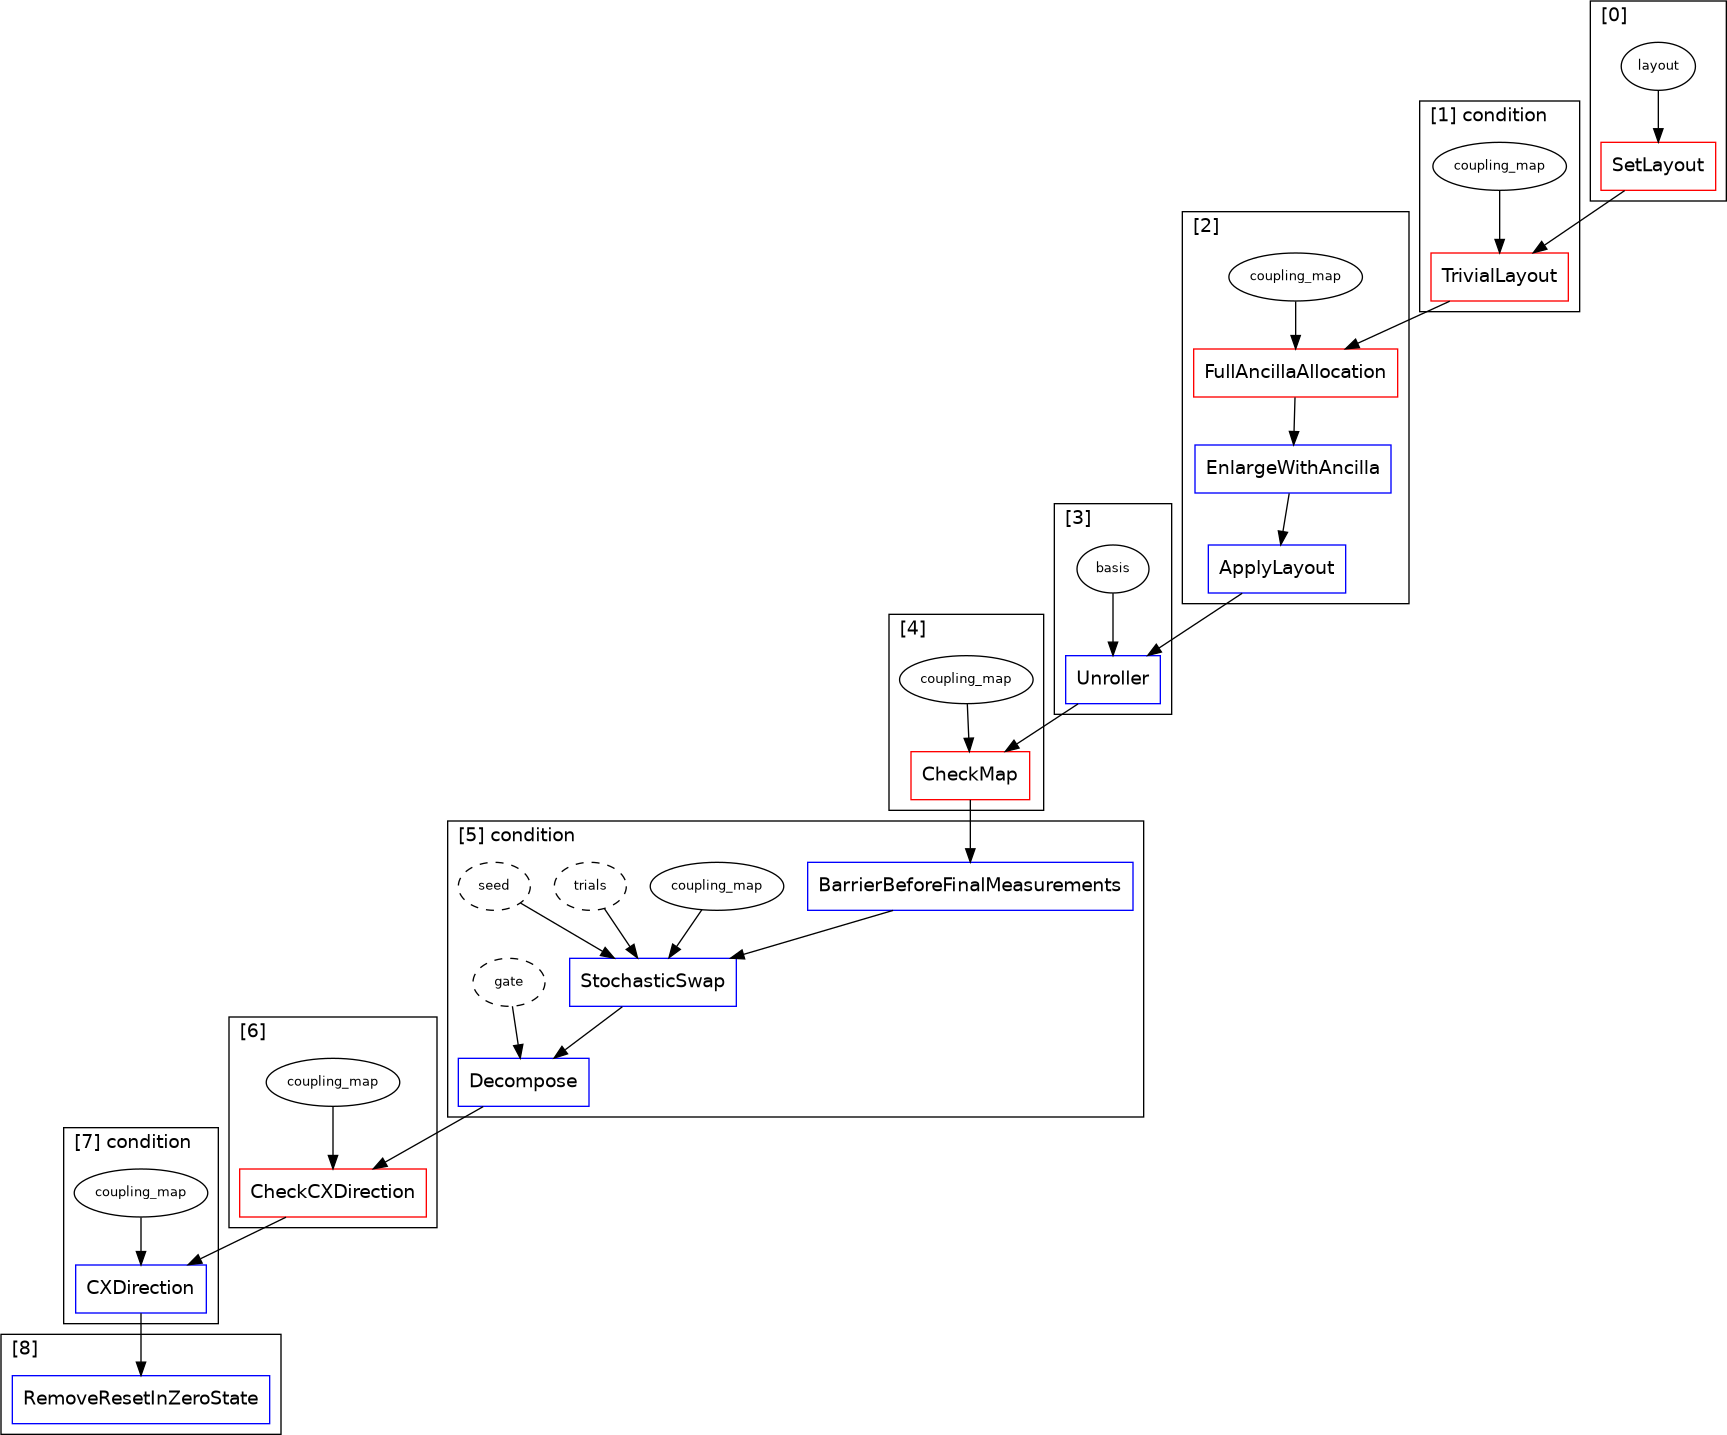
\includegraphics[width=\textwidth,height=\textheight,keepaspectratio]{preset_level_0.png}
    \end{columns}}
    \only<2>{
    \textbf{Optimization Level 1}\\
    \begin{columns}
        \column{.5\textwidth}
        \begin{itemize}
            \item Unroll
            \item Trivial Layout
            \item Swap Mapping
            \item Optimization
                \begin{itemize}
                    \item Optimize 1Q
                    \item CX Cancellation
                \end{itemize}
        \end{itemize}
        \column{.5\textwidth}
        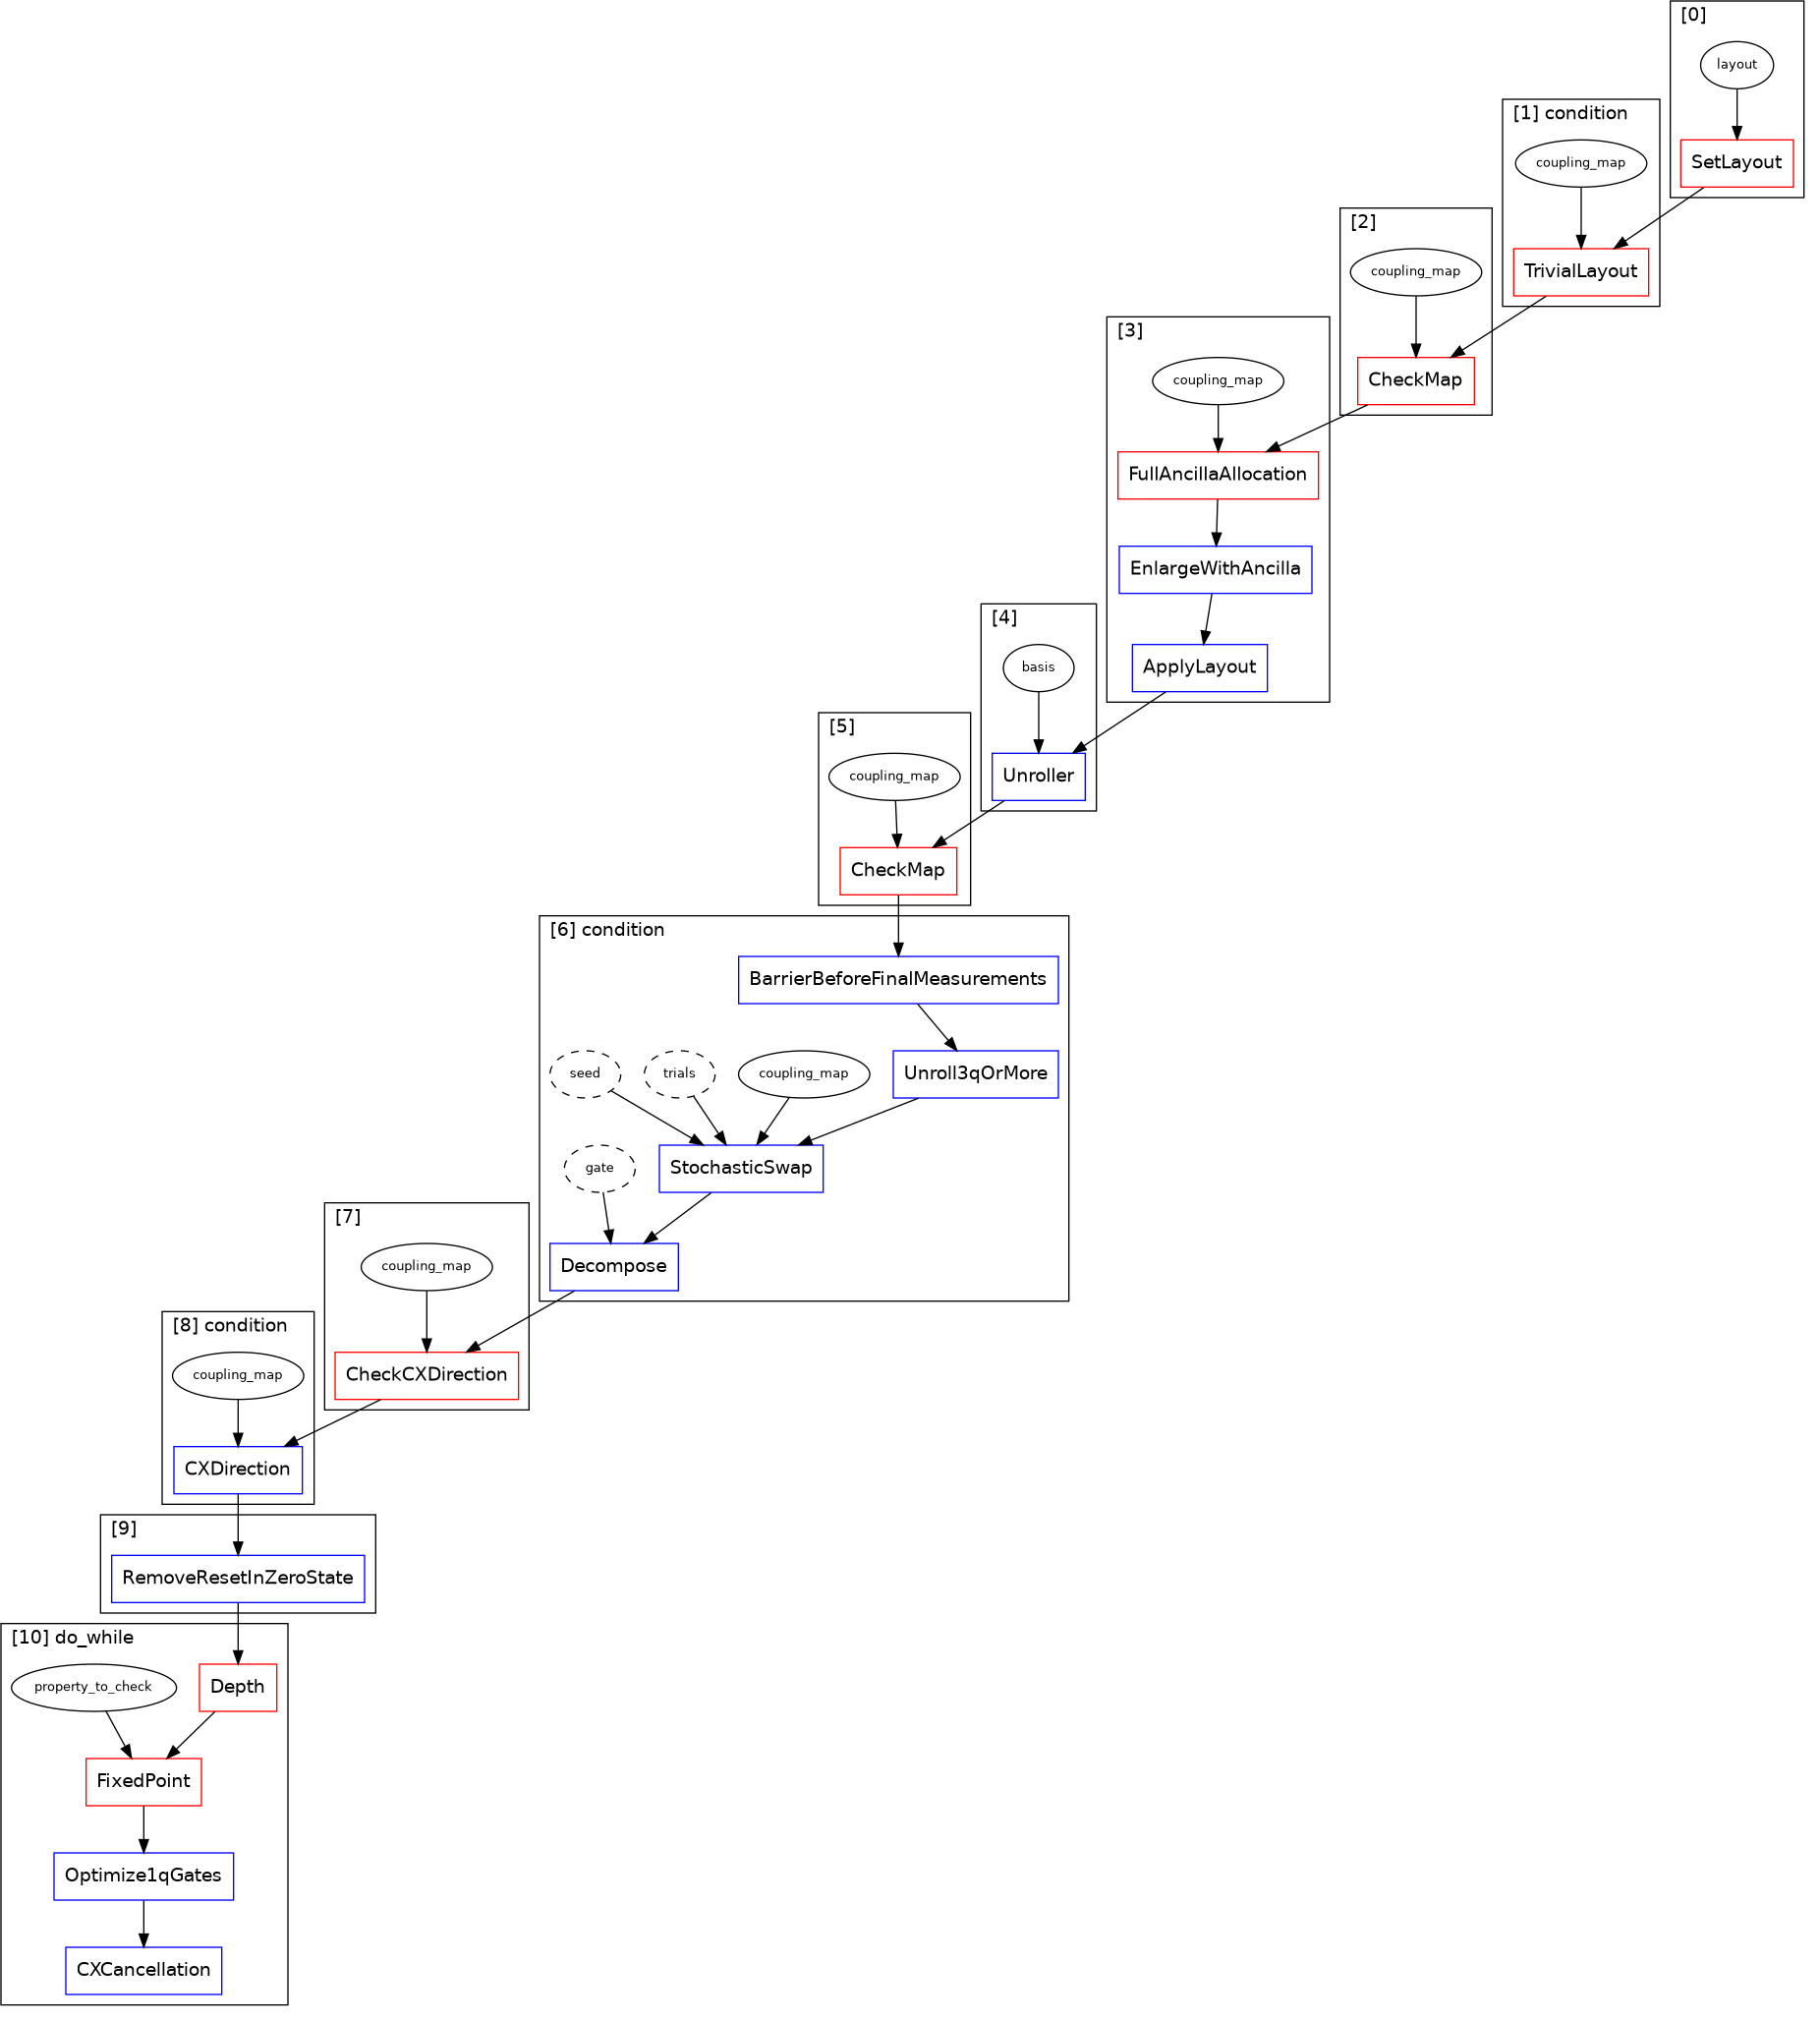
\includegraphics[width=\textwidth,height=\textheight,keepaspectratio]{preset_level_1.png}
    \end{columns}
    }
    \only<3>{
    \textbf{Optimization Level 2}\\
    \begin{columns}
        \column{.5\textwidth}
        \begin{itemize}
            \item Unroll
            \item Dense Layout
            \item Swap Mapping
            \item Optimization
                \begin{itemize}
                    \item Optimize 1Q
                    \item Commutative Cancellation
                \end{itemize}
        \end{itemize}
        \column{.5\textwidth}
            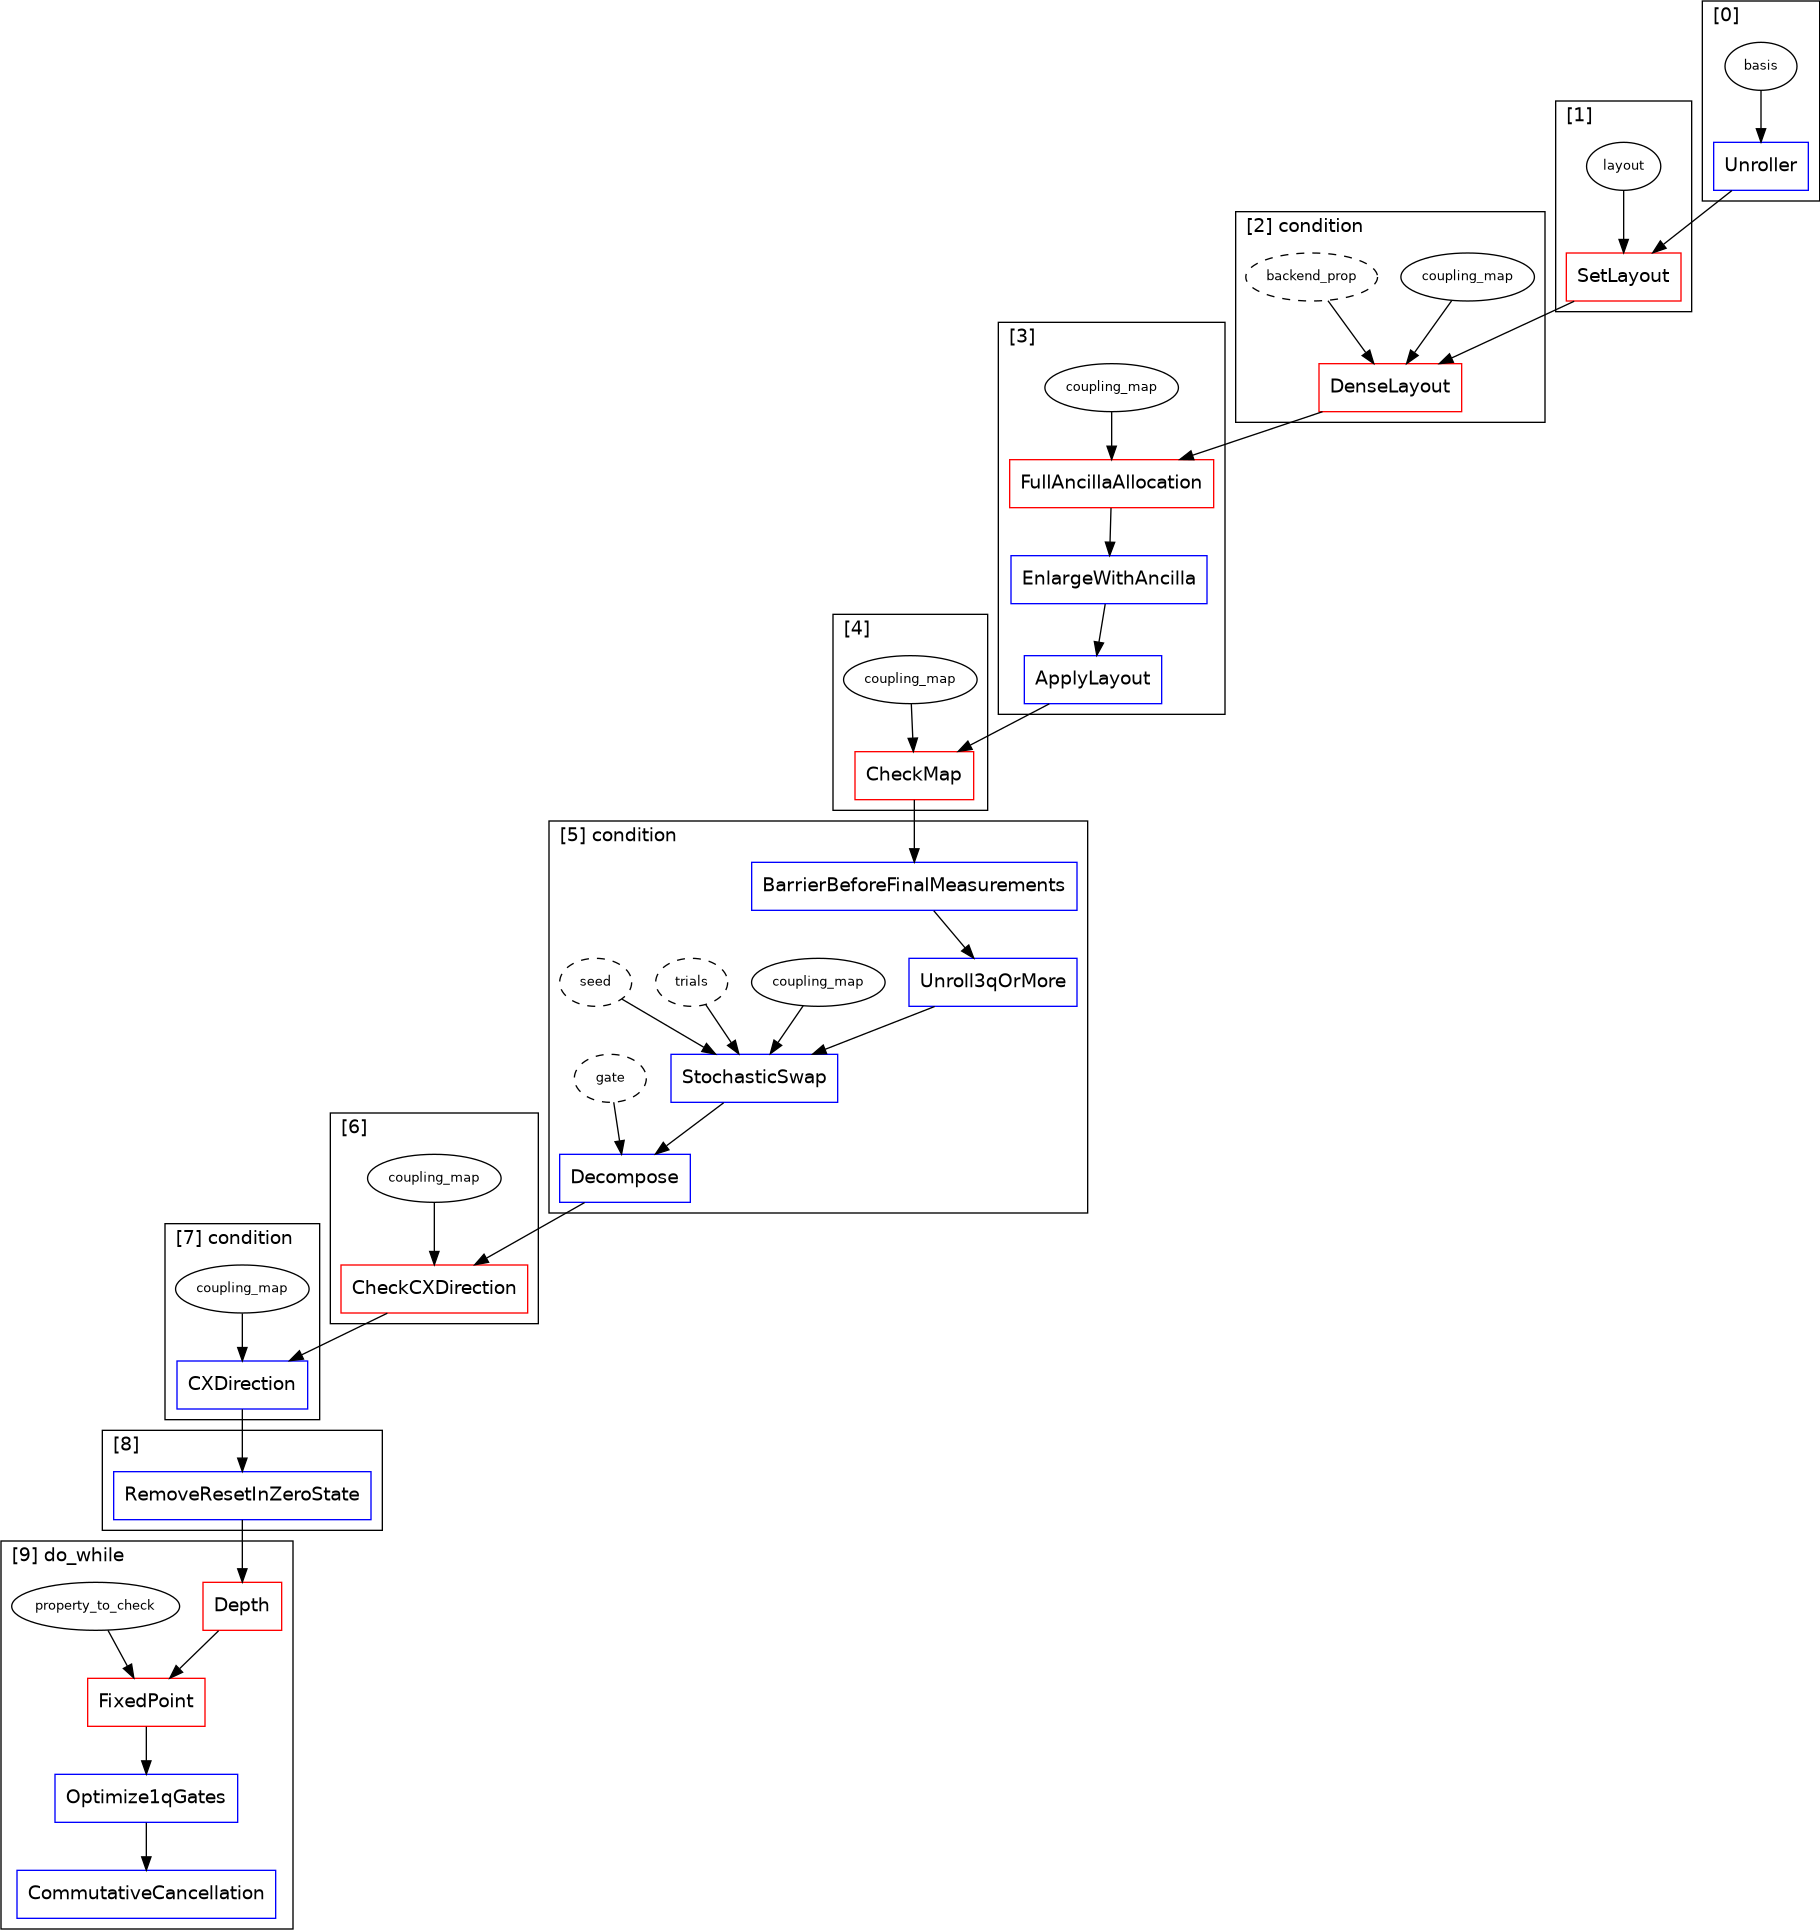
\includegraphics[width=\textwidth,height=\textheight,keepaspectratio]{preset_level_2.png}
    \end{columns}
    }
    \only<4>{
        \textbf{Optimization Level 3}\\
    \begin{columns}
        \column{.5\textwidth}
        \begin{itemize}
            \item Unroll
            \item Noise Aware Layout
            \item Swap Mapping
            \item Optimization
                \begin{itemize}
                    \item Optimize 1Q
                    \item Commutative Cancellation
                    \item Consolidate Blocks
                    \item Remove Reset in 0 State
                    \item Optimize Swap before measure
                    \item Remove Diagonal Gates before measure
                \end{itemize}
        \end{itemize}
        \column{.5\textwidth}
            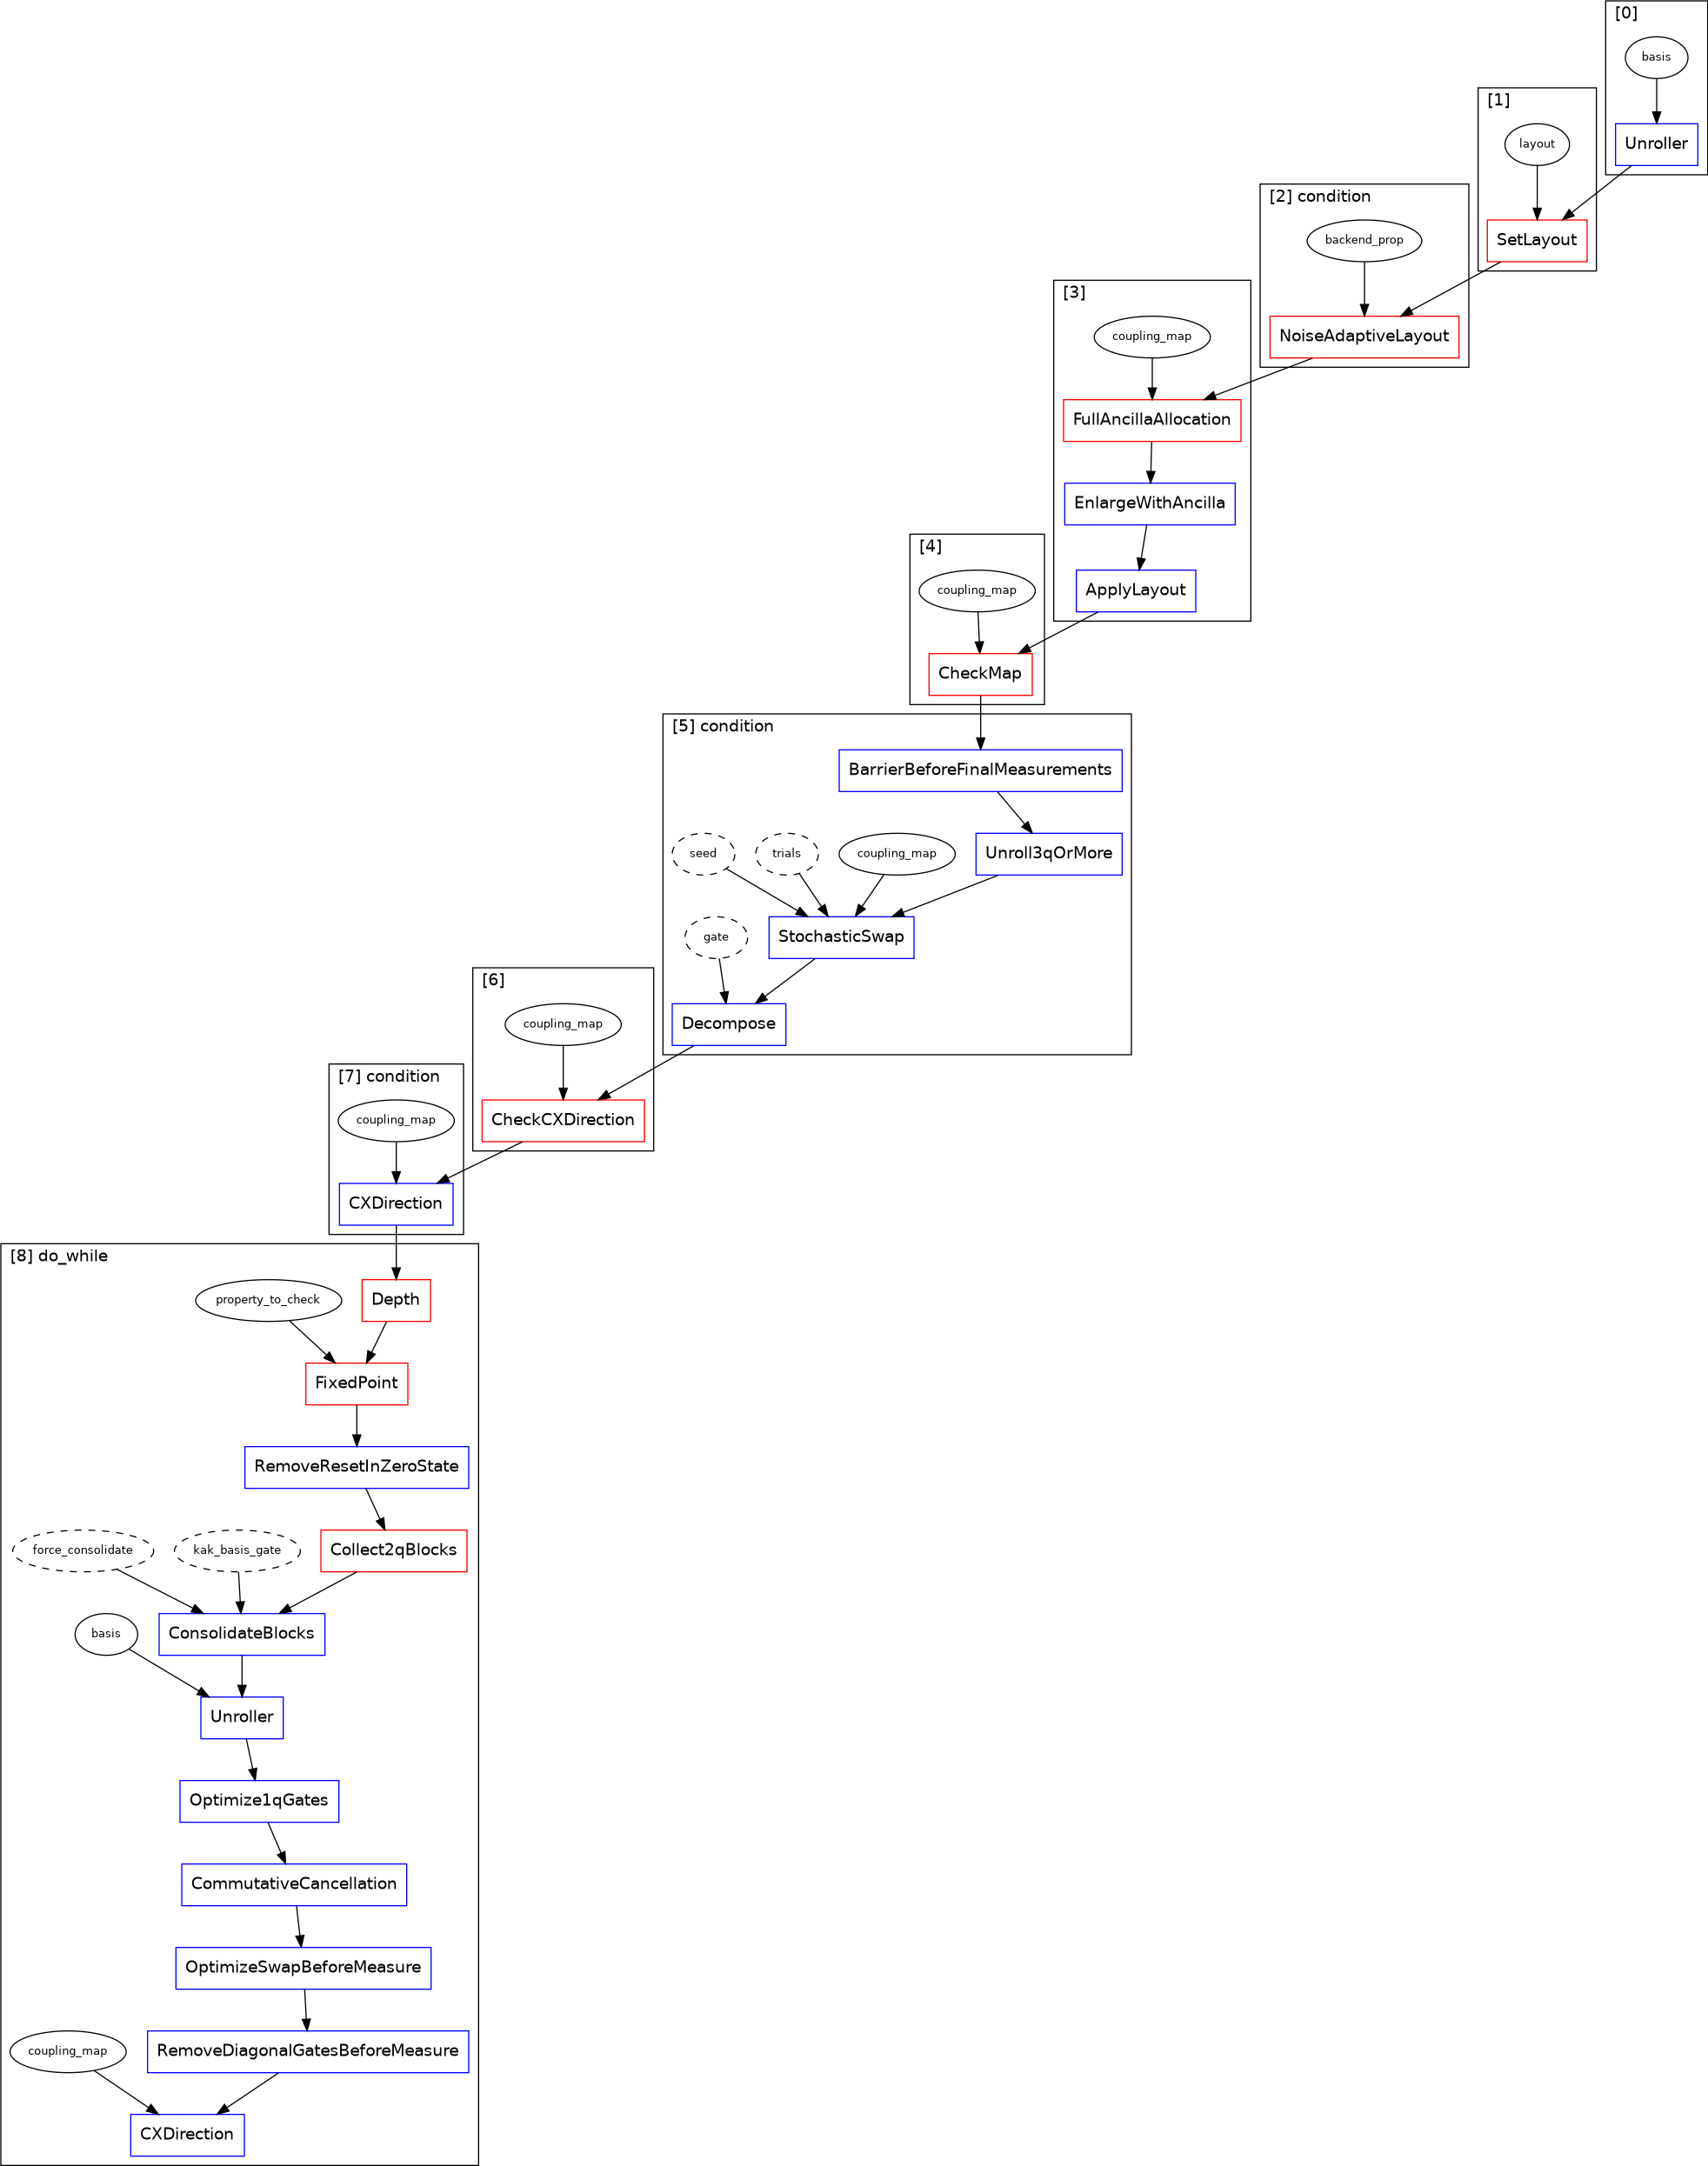
\includegraphics[width=\textwidth,height=\textheight,keepaspectratio]{preset_level_3.png}
    \end{columns}
    }
\end{frame}

\section{Passes}
\subsection{Unroller}
\begin{frame}
    \frametitle{The Unroller}
    \begin{columns}
        \column{.5\textwidth}
        \begin{itemize}
            \item The first stage of any compilation is to unroll the gates to
                the basis set
            \item Currently this is done using a descent tree
            \item Mainly works for superconducting qubit basis
            \item Other types of devices support is hardcoded extra path
        \end{itemize}
        \column{.5\textwidth}
            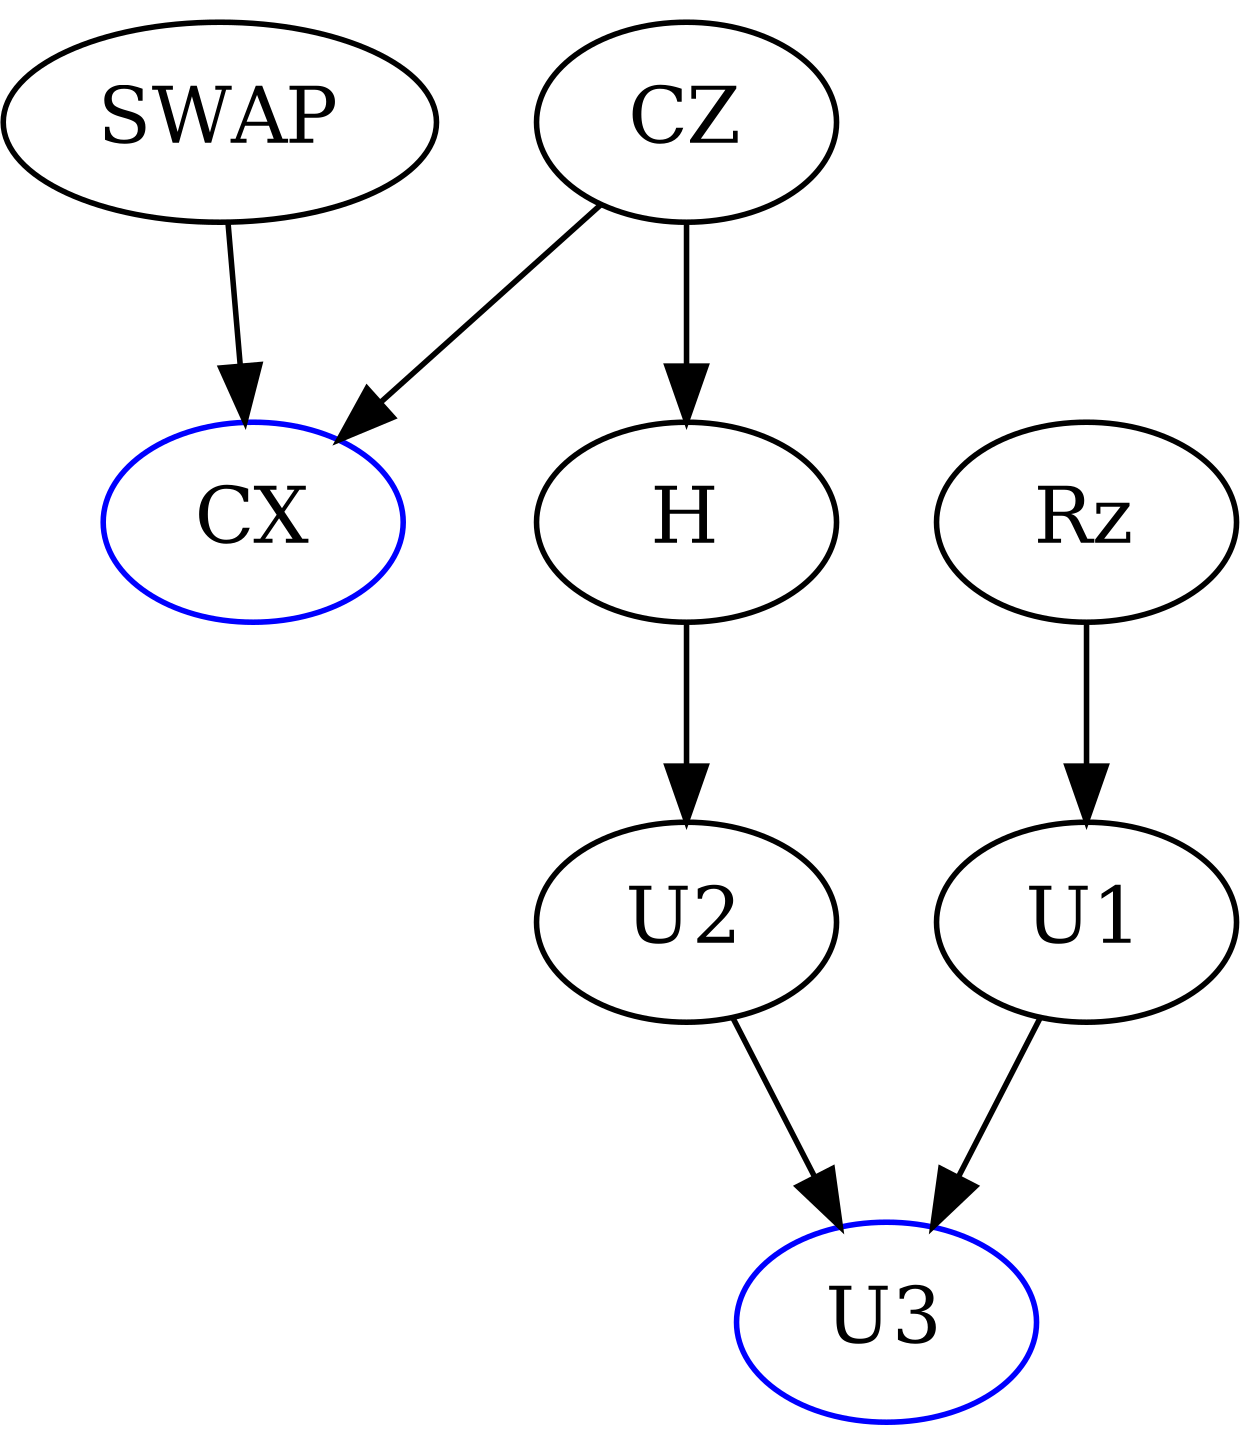
\includegraphics[width=\textwidth]{unroll_descent.png}
    \end{columns}
\end{frame}

\subsection{Layout}
\begin{frame}
    \frametitle{Layout}
    \begin{columns}
        \column{.45\textwidth}
            \begin{itemize}
                \item Initial mapping to physical qubits
                \item Multiple options included
                    \begin{itemize}
                        \item \href{https://github.com/Qiskit/qiskit-terra/blob/master/qiskit/transpiler/passes/layout/trivial\_layout.py}{TrivialLayout}
                        \item \href{https://github.com/Qiskit/qiskit-terra/blob/master/qiskit/transpiler/passes/layout/dense\_layout.py}{DenseLayout}
                        \item \href{https://github.com/Qiskit/qiskit-terra/blob/master/qiskit/transpiler/passes/layout/noise\_adaptive\_layout.py}{NoiseAdaptiveLayout}
                    \end{itemize}
            \end{itemize}
        \column{.45\textwidth}
            \centering
            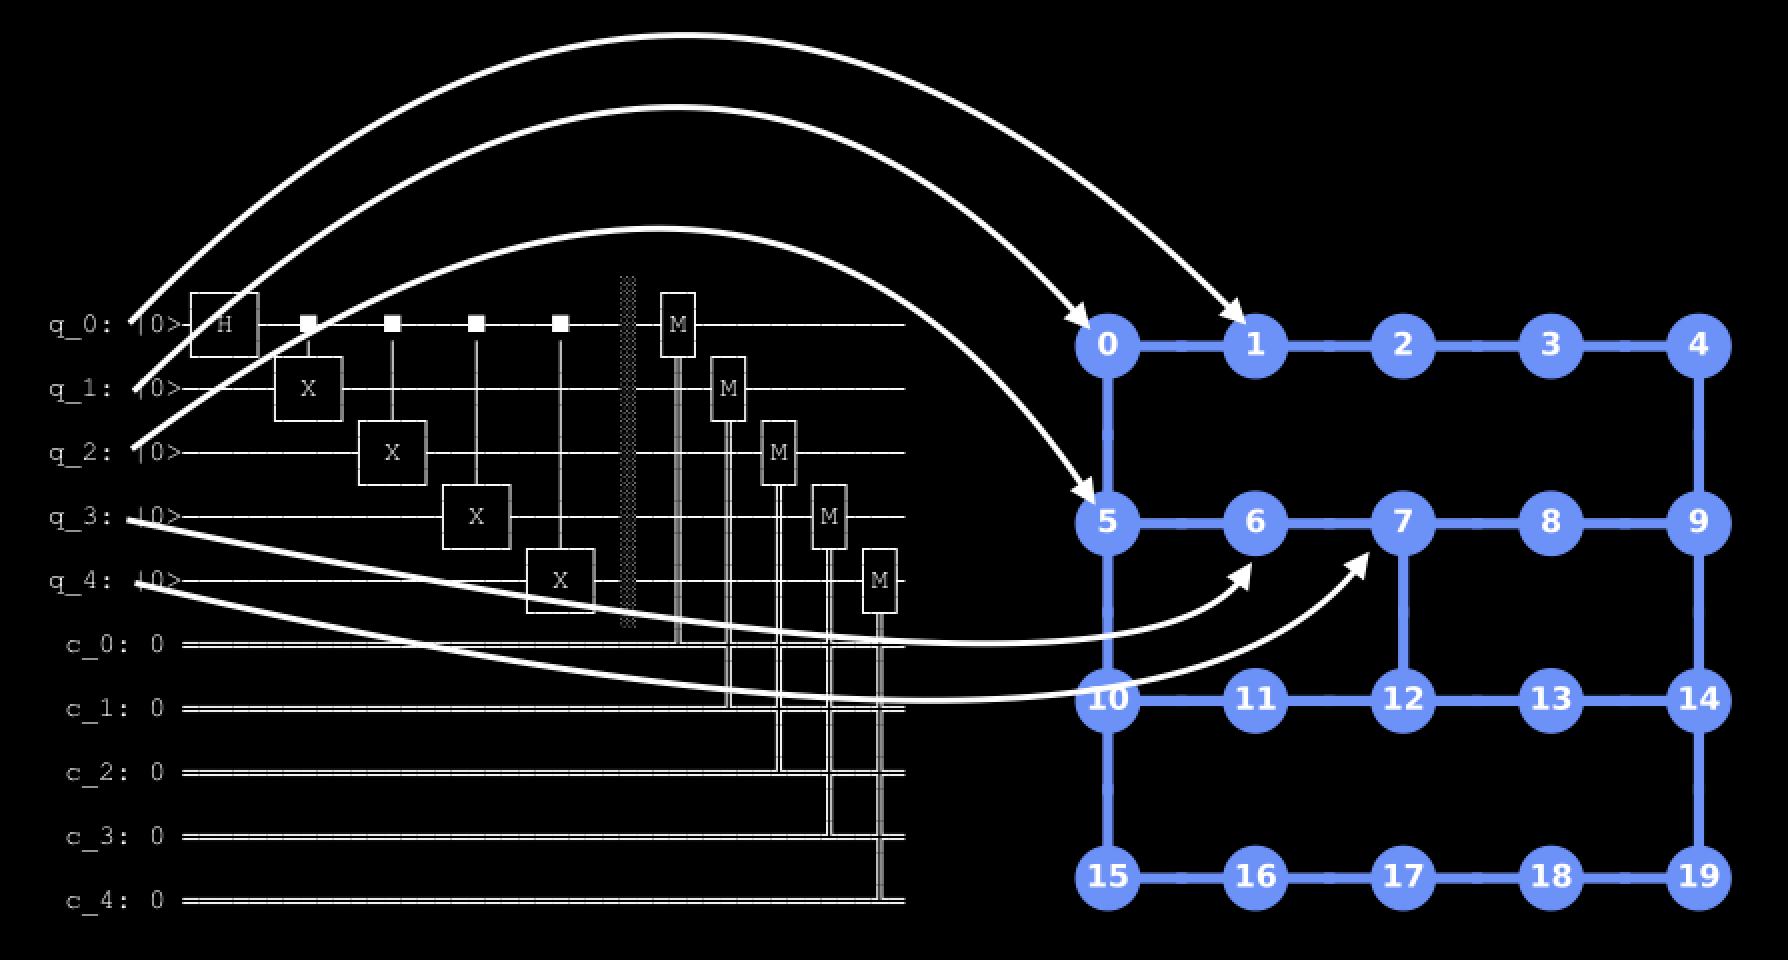
\includegraphics[width=1.1\textwidth]{layout.png}
    \end{columns}
\end{frame}

\begin{frame}
    \frametitle{Layout Example}
    \begin{columns}
        \column{.45\textwidth}
            \centering
            \textbf{Logical Circuit}
            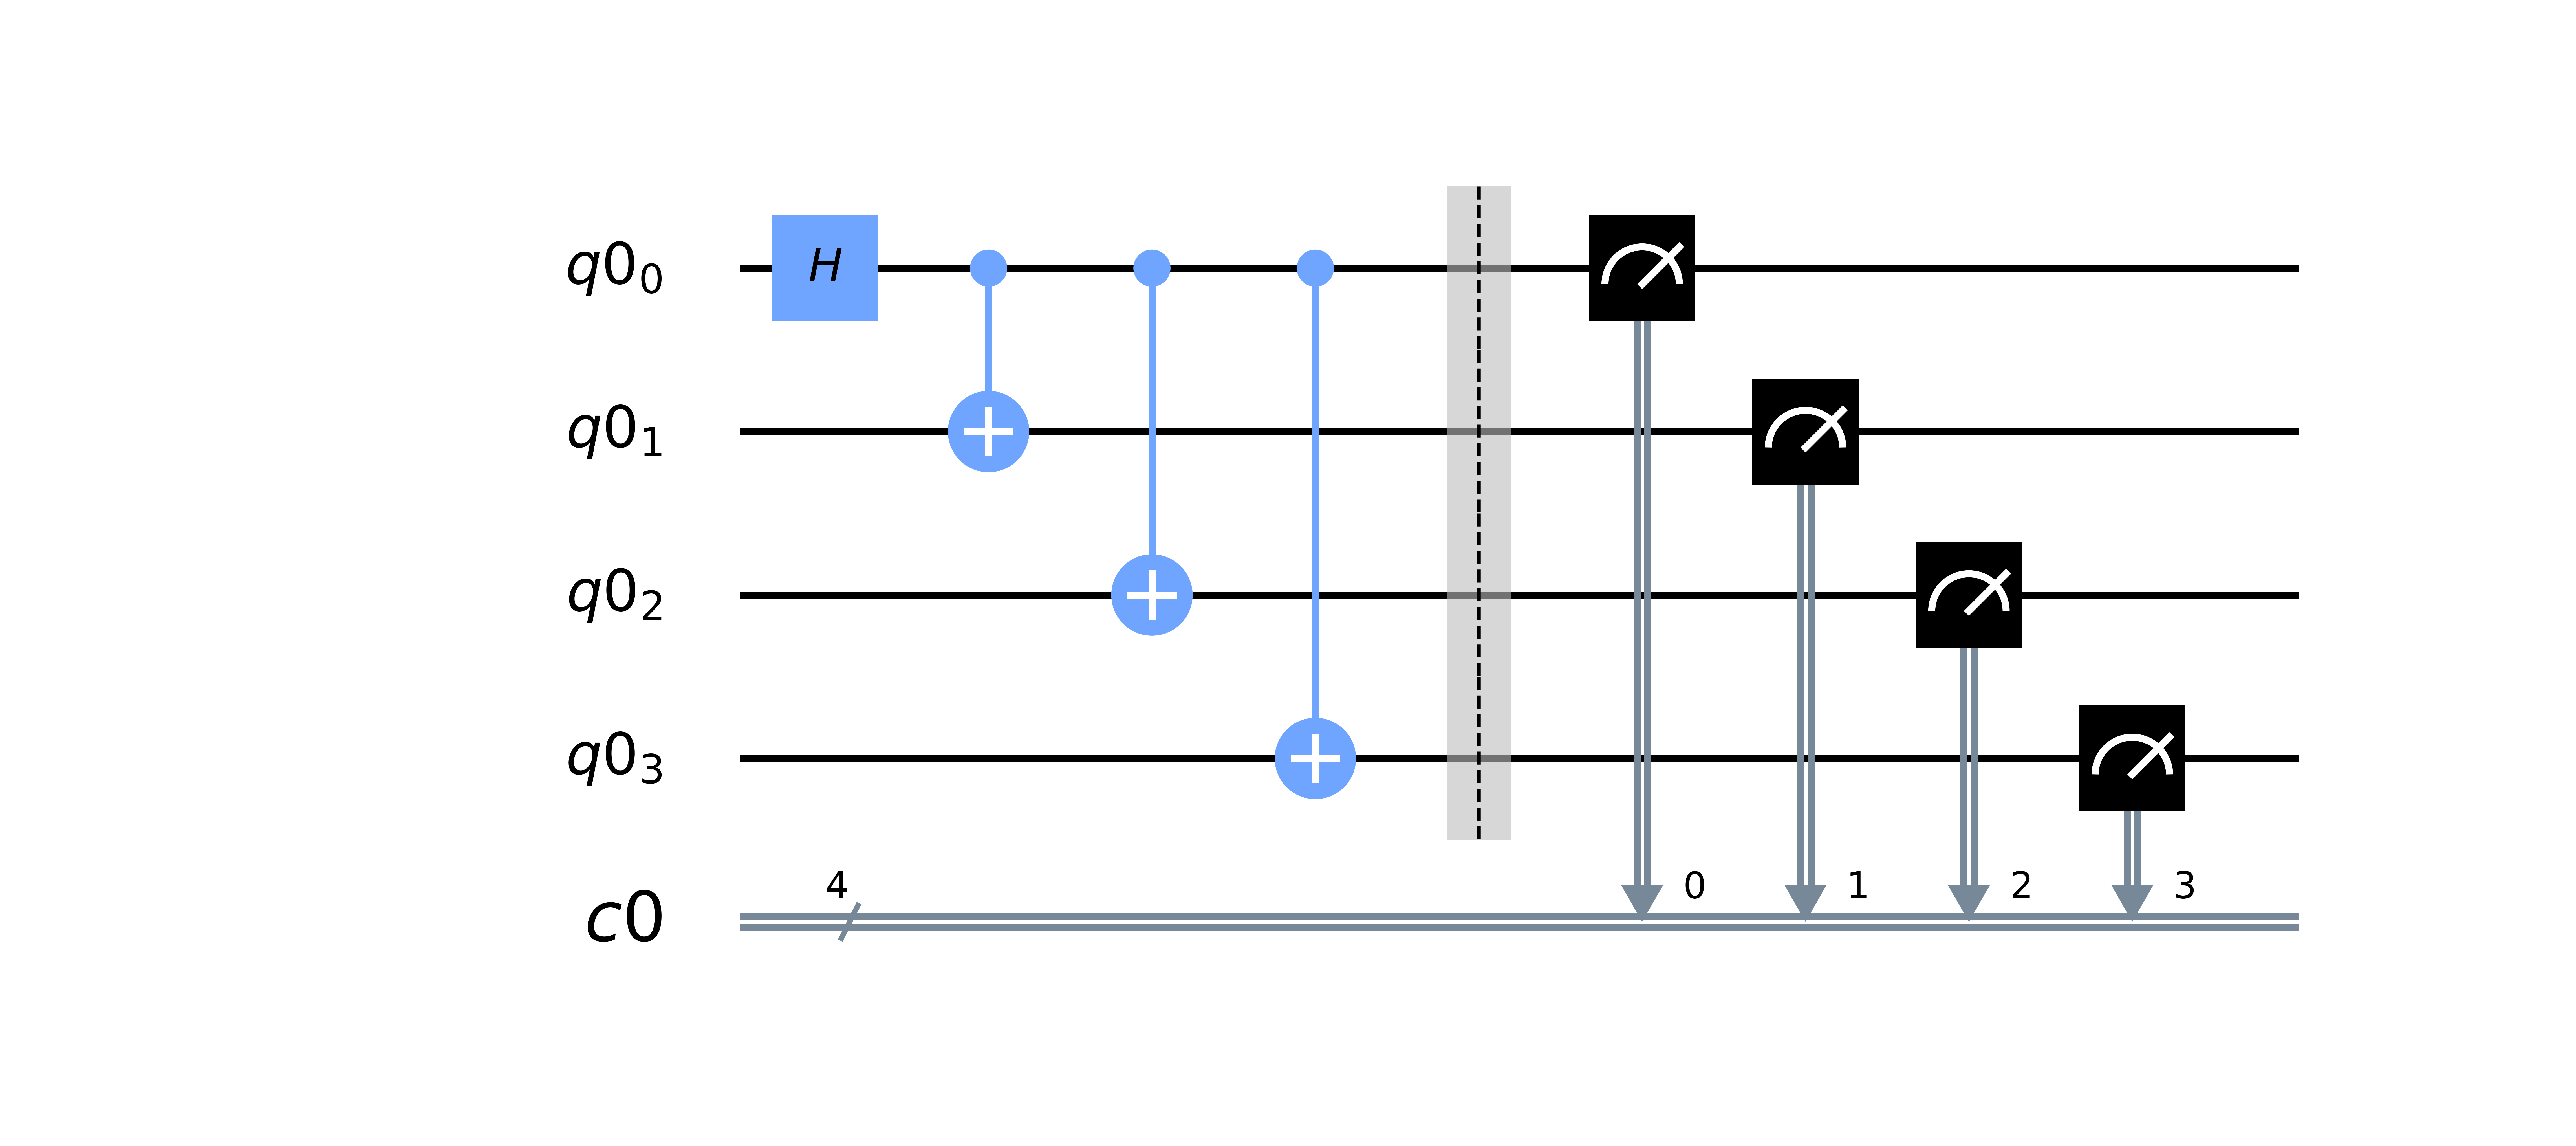
\includegraphics[width=\textwidth]{no_layout.png}
        \column{.45\textwidth}
            \centering
            \textbf{Target Device}
            \only<1>{\includegraphics[width=\textwidth]{ibmqx2-labeled.png}}
            \only<2>{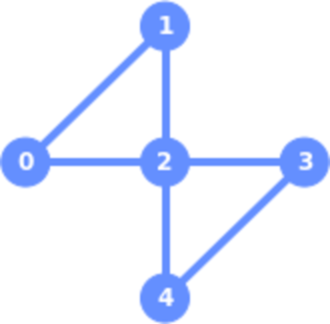
\includegraphics[width=.7\textwidth]{layout_device.png}}
    \end{columns}
\end{frame}


\begin{frame}
    \begin{columns}
        \column{.5\textwidth}
            \centering
            optimization\_level=1\\
            TrivialLayout\\
            \includegraphics[width=\textwidth, height=.6\textheight, keepaspectratio]{layout_1.png}\\
            optimization\_level=2\\
            DenseLayout\\
            \includegraphics[width=\textwidth, height=.6\textheight, keepaspectratio]{layout_2.png}

        \column{.5\textwidth}
            \centering
            optimization\_level=3\\
            NoiseAdaptiveLayout\\
            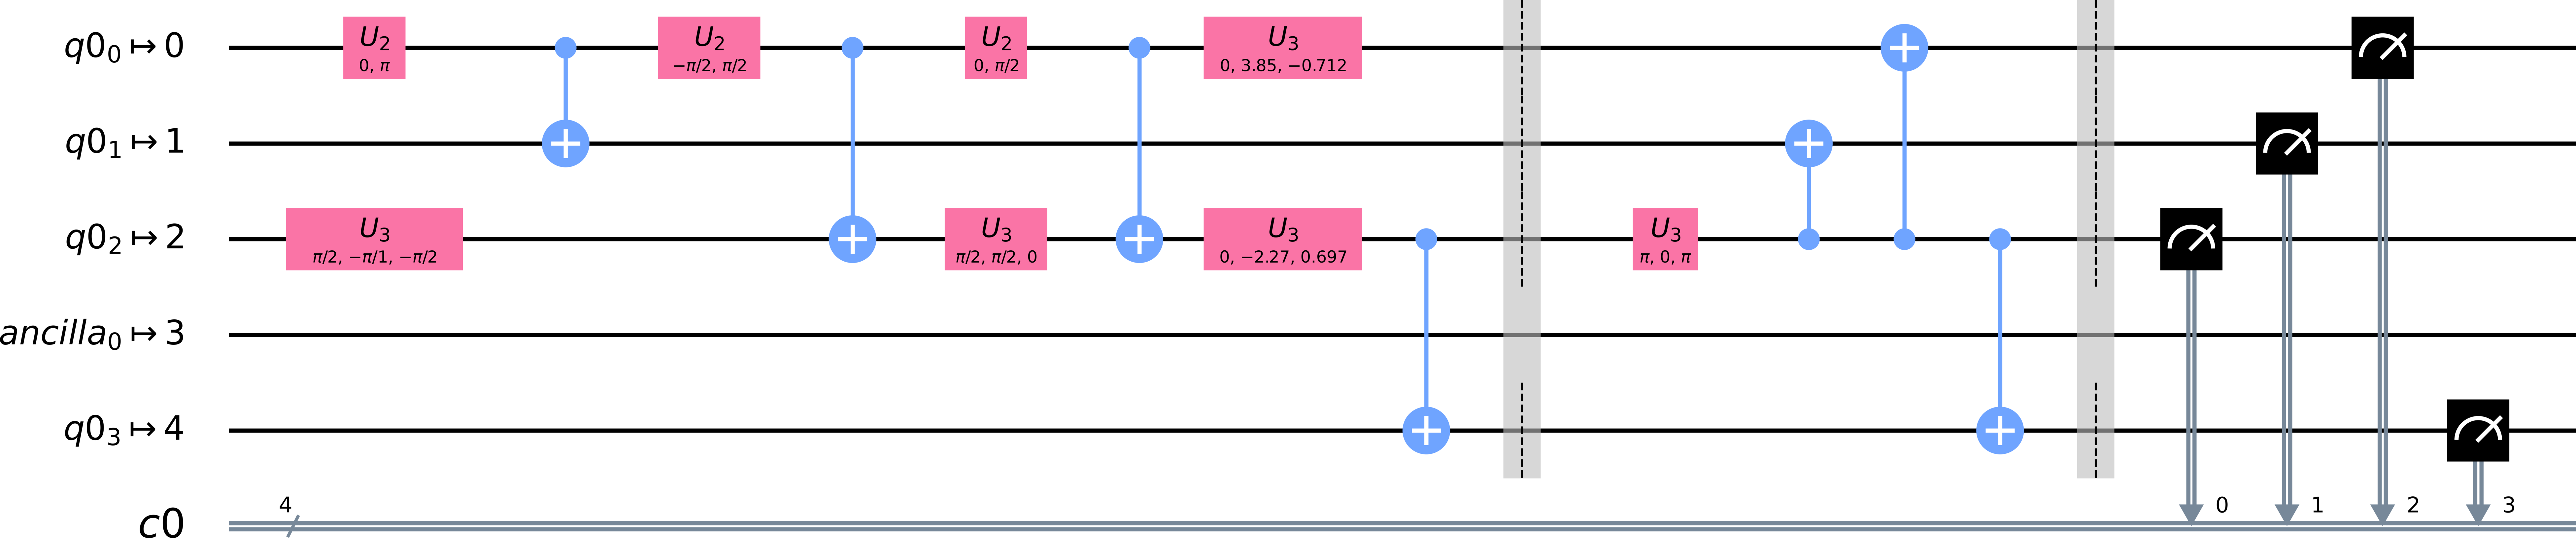
\includegraphics[width=\textwidth, height=.6\textheight, keepaspectratio]{layout_3.png}\\
            Custom Layout\\
            (optimization\_level=1)\\
            \includegraphics[width=\textwidth, height=.6\textheight, keepaspectratio]{custom_layout.png}
    \end{columns}
\end{frame}

\begin{frame}
    \begin{columns}
        \column{.5\textwidth}
            \centering
            optimization\_level=1\\
            TrivialLayout\\
            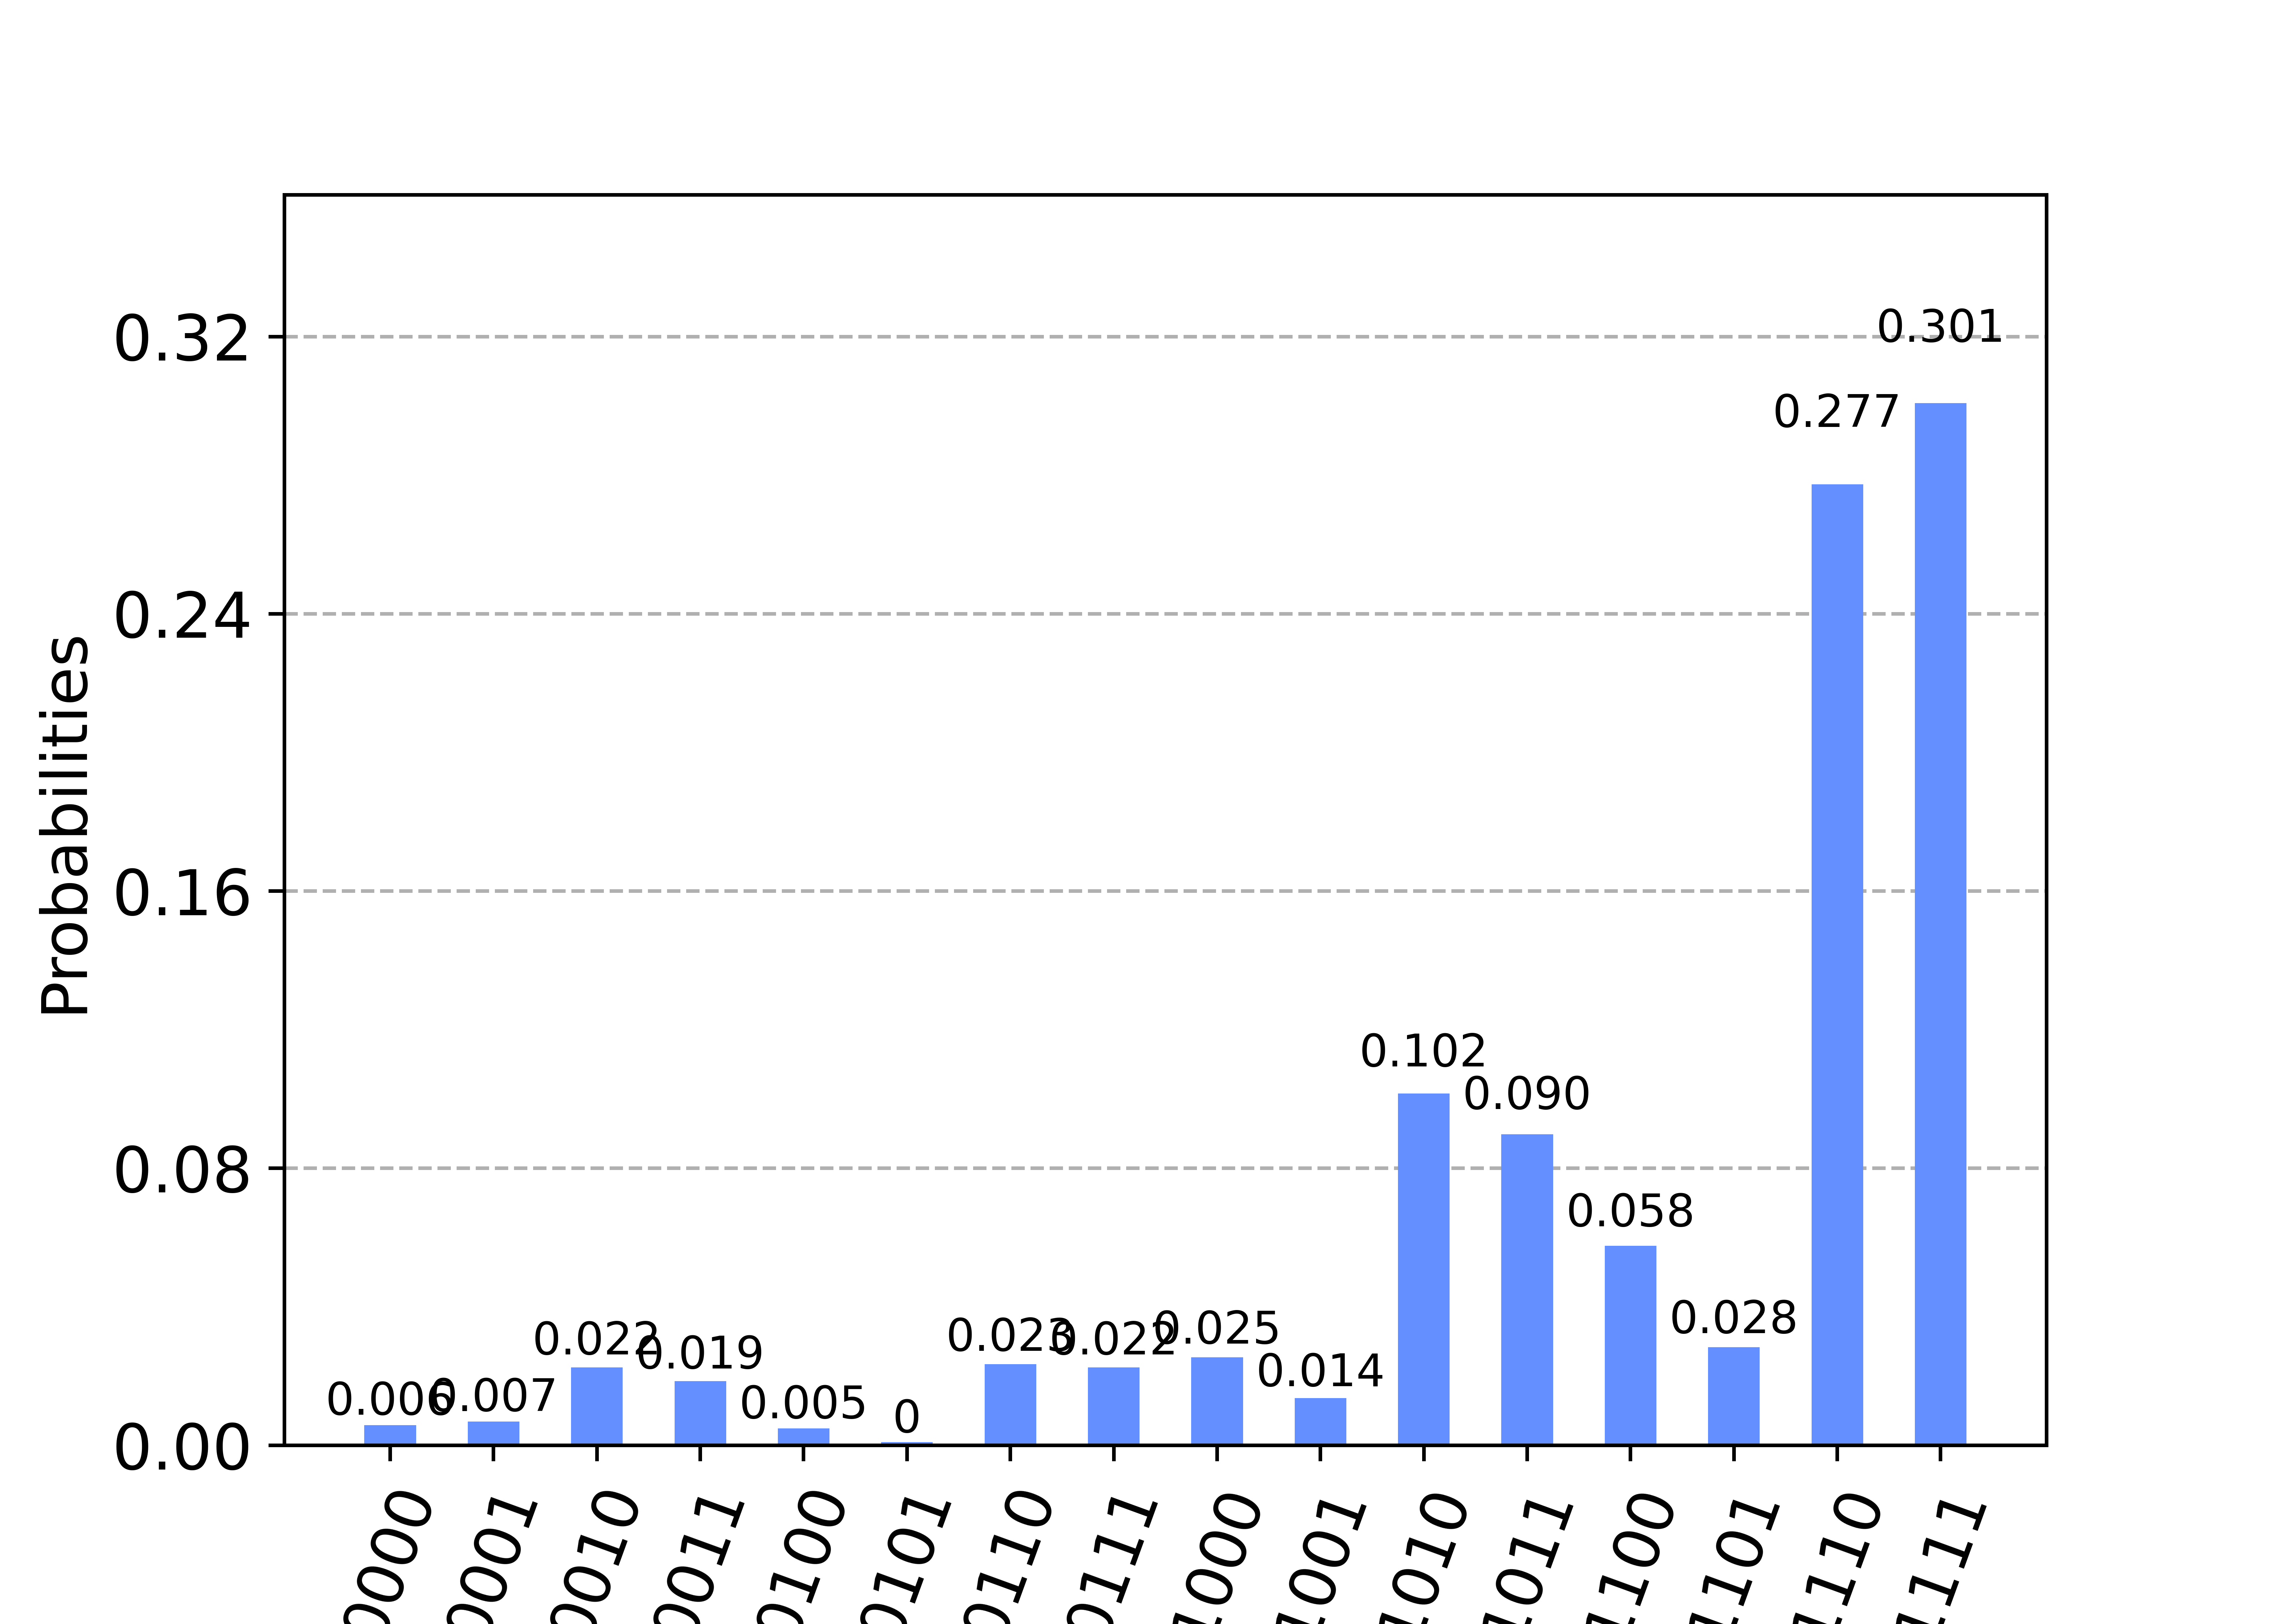
\includegraphics[width=\textwidth, height=.4\textheight, keepaspectratio]{layout_1_results.png}\\
            optimization\_level=2\\
            DenseLayout\\
        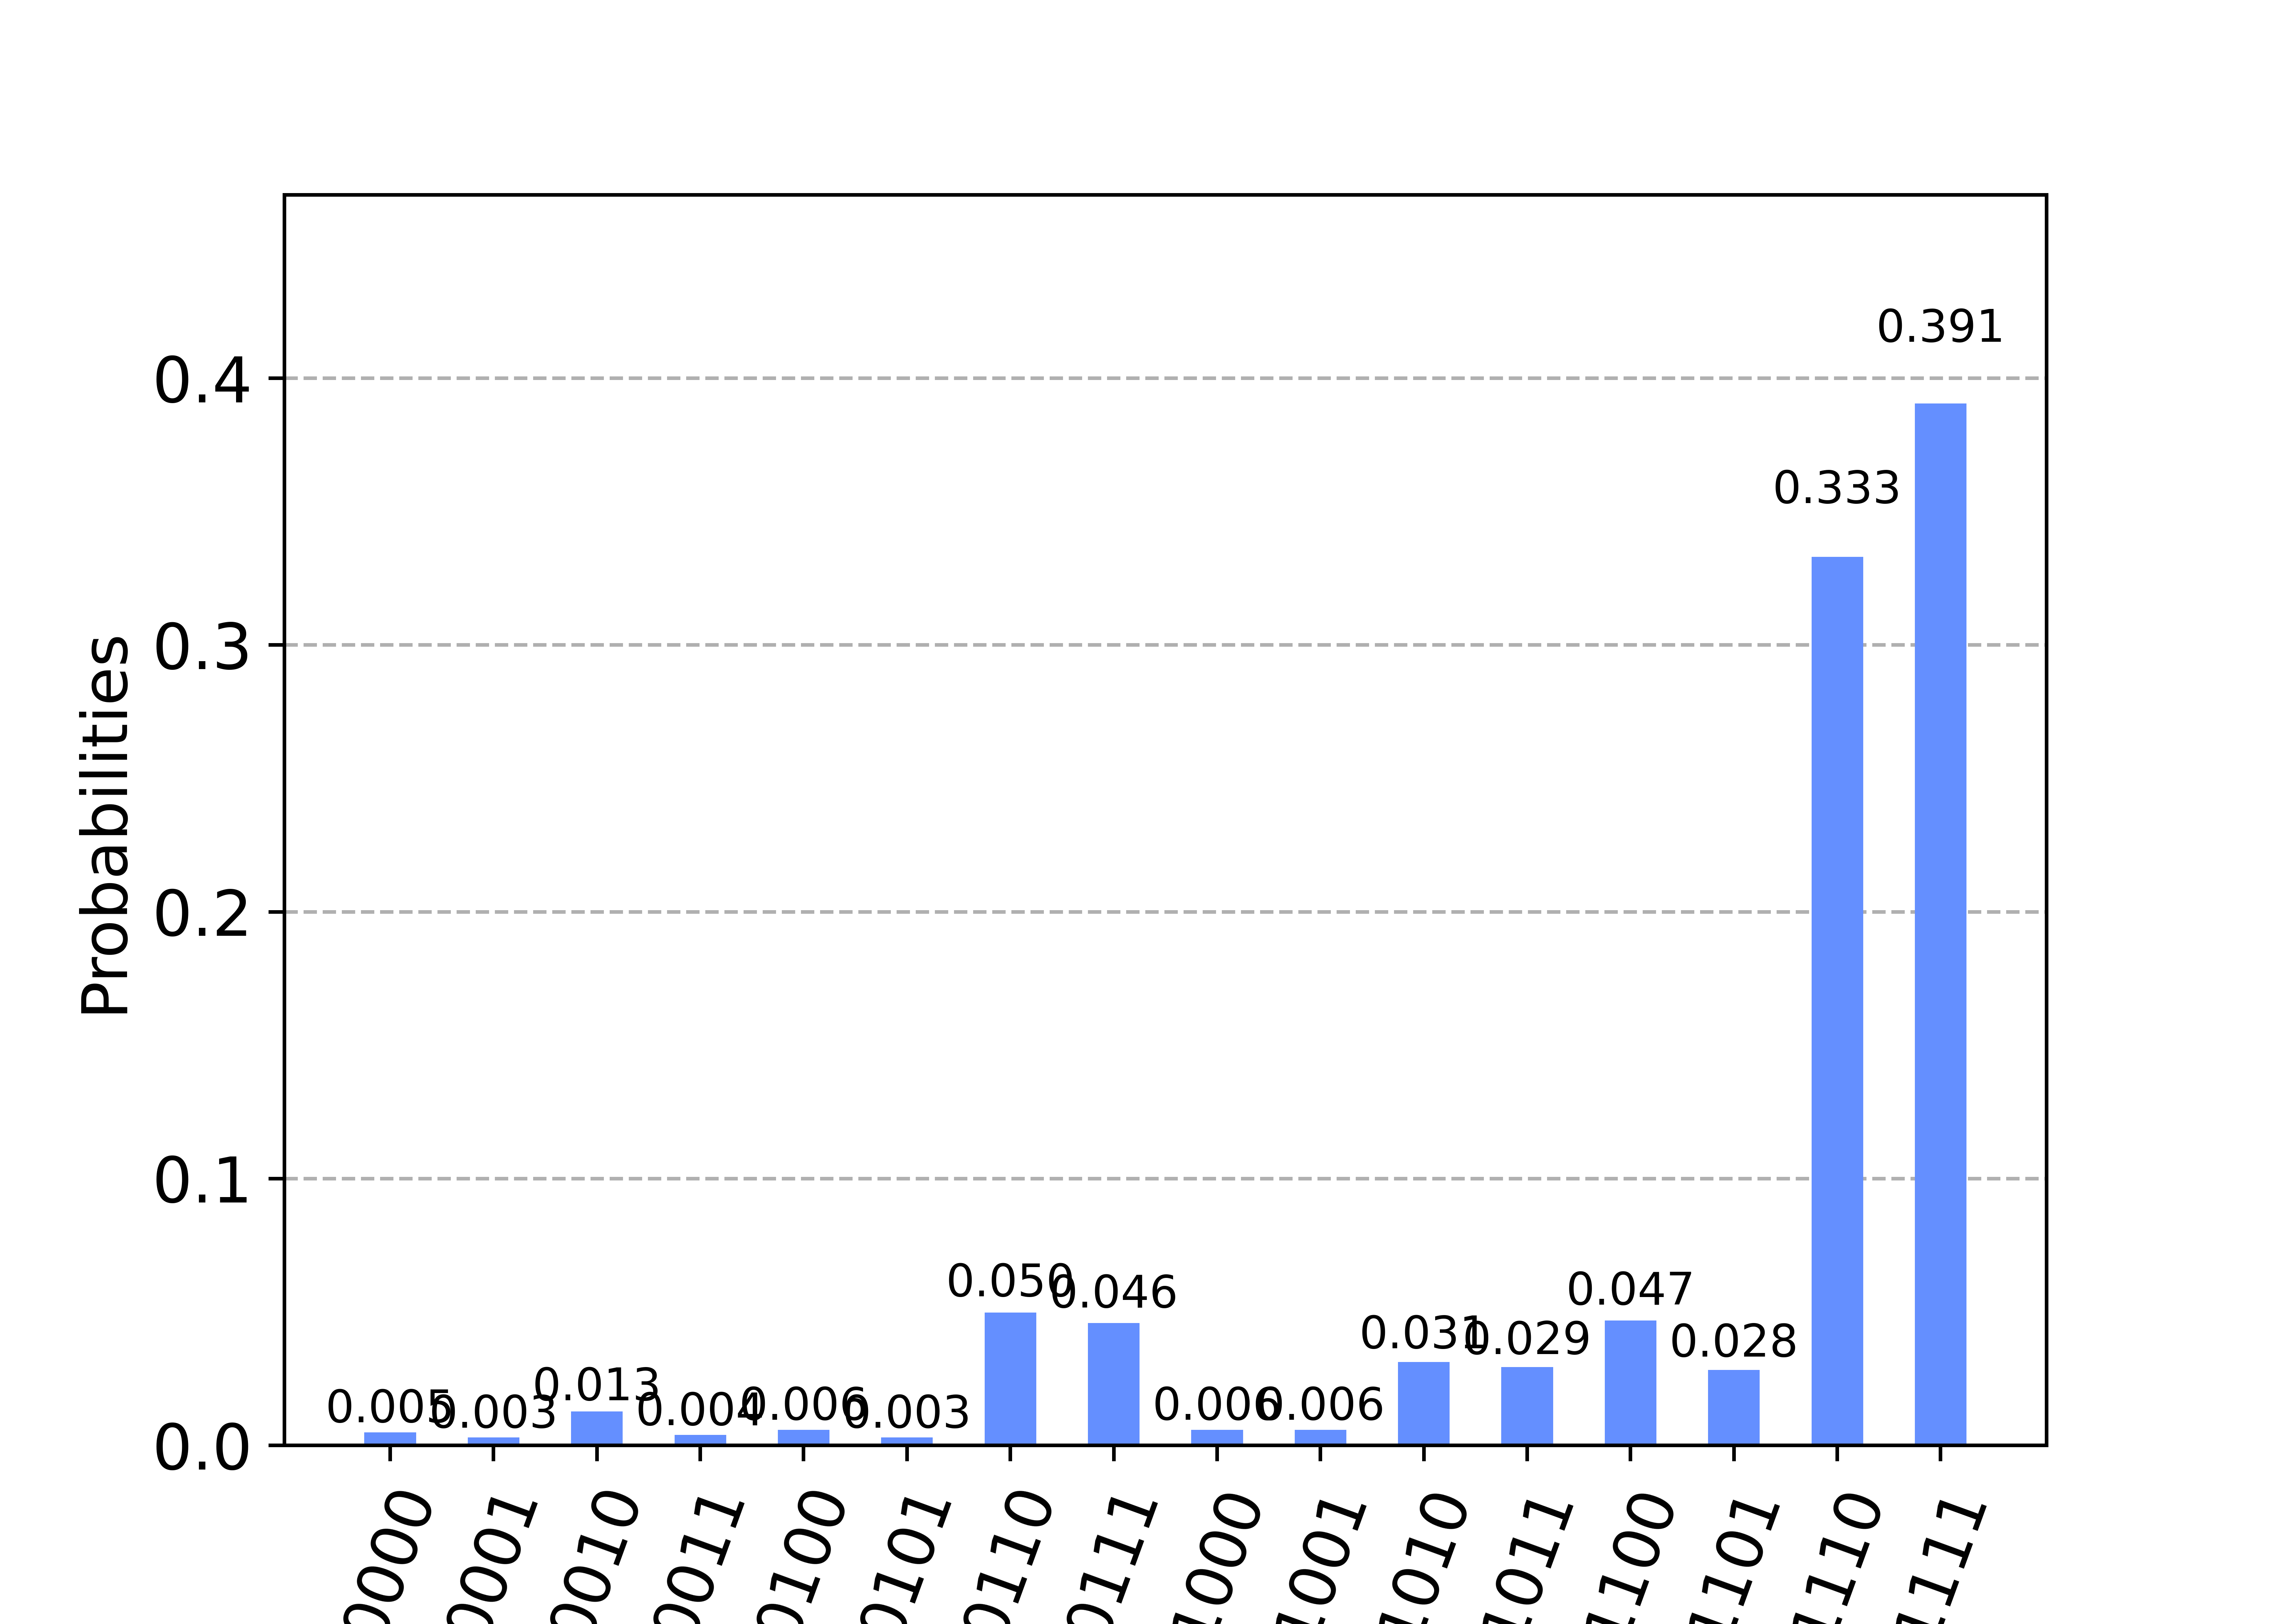
\includegraphics[width=\textwidth, height=.4\textheight, keepaspectratio]{layout_2_results.png}

        \column{.5\textwidth}
            \centering
            optimization\_level=3\\
            NoiseAdaptiveLayout\\
            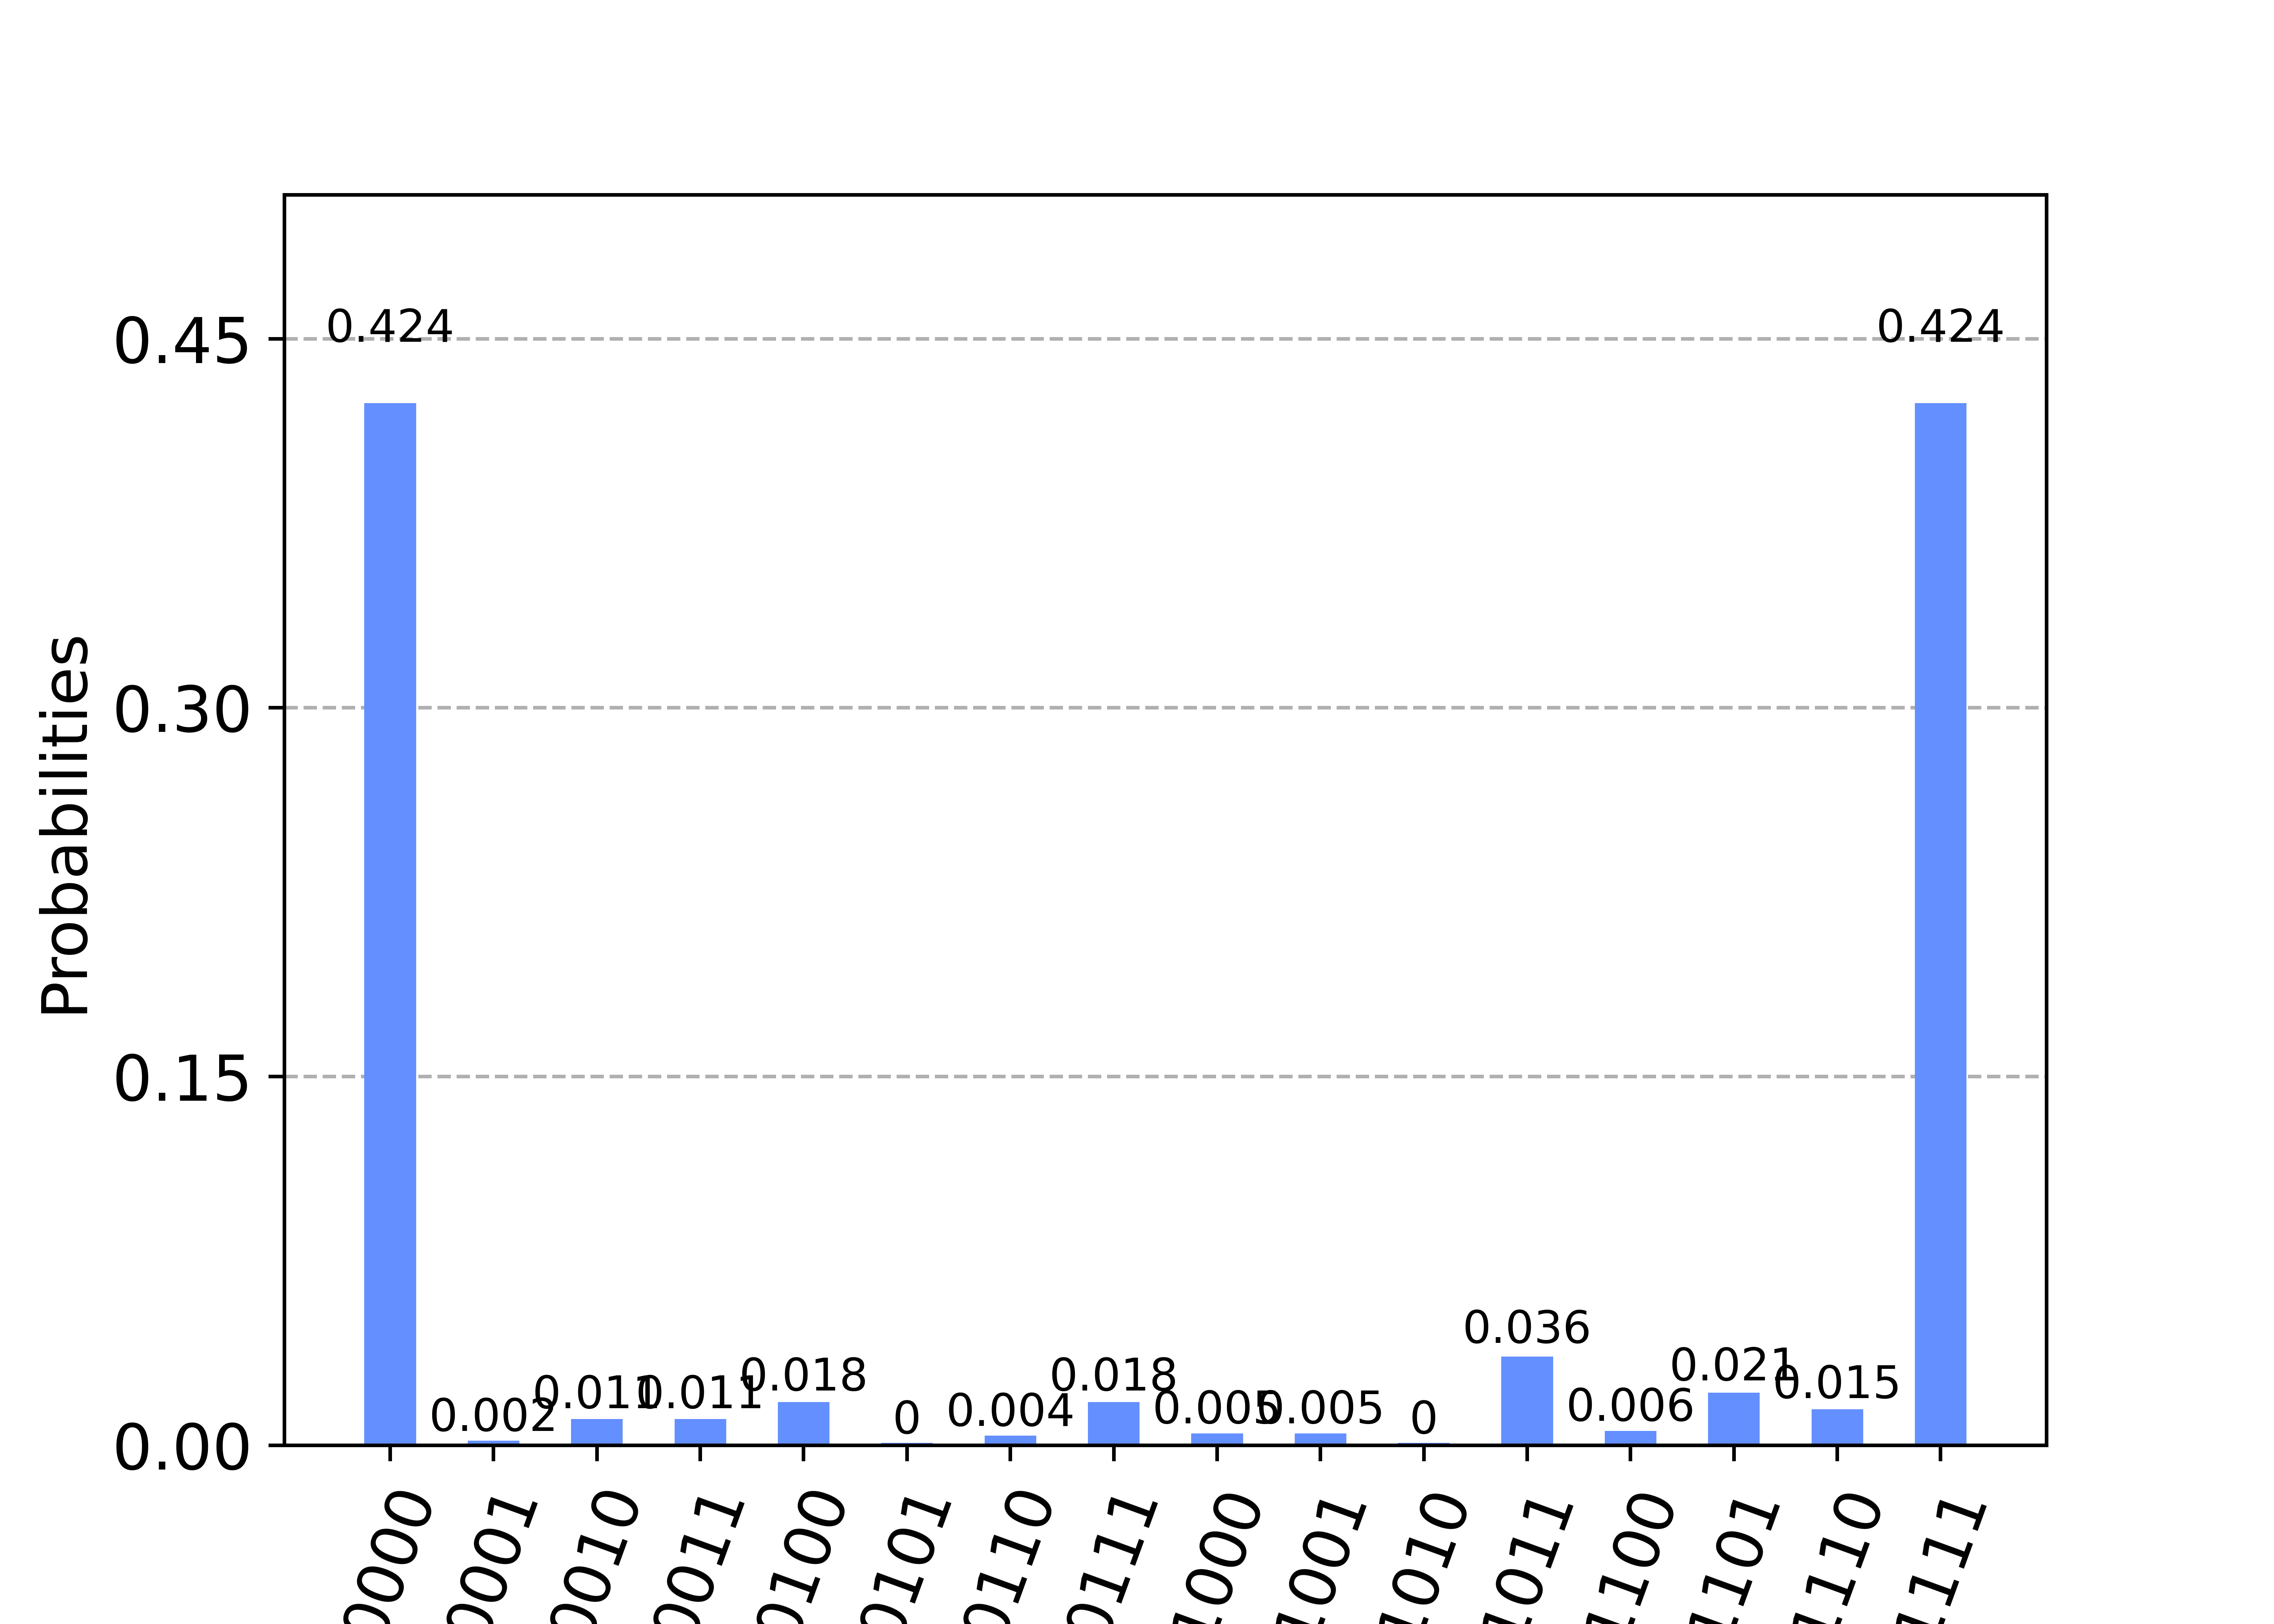
\includegraphics[width=\textwidth, height=.4\textheight, keepaspectratio]{layout_3_results.png}\\
            Custom Layout\\
            (optimization\_level=1)\\
            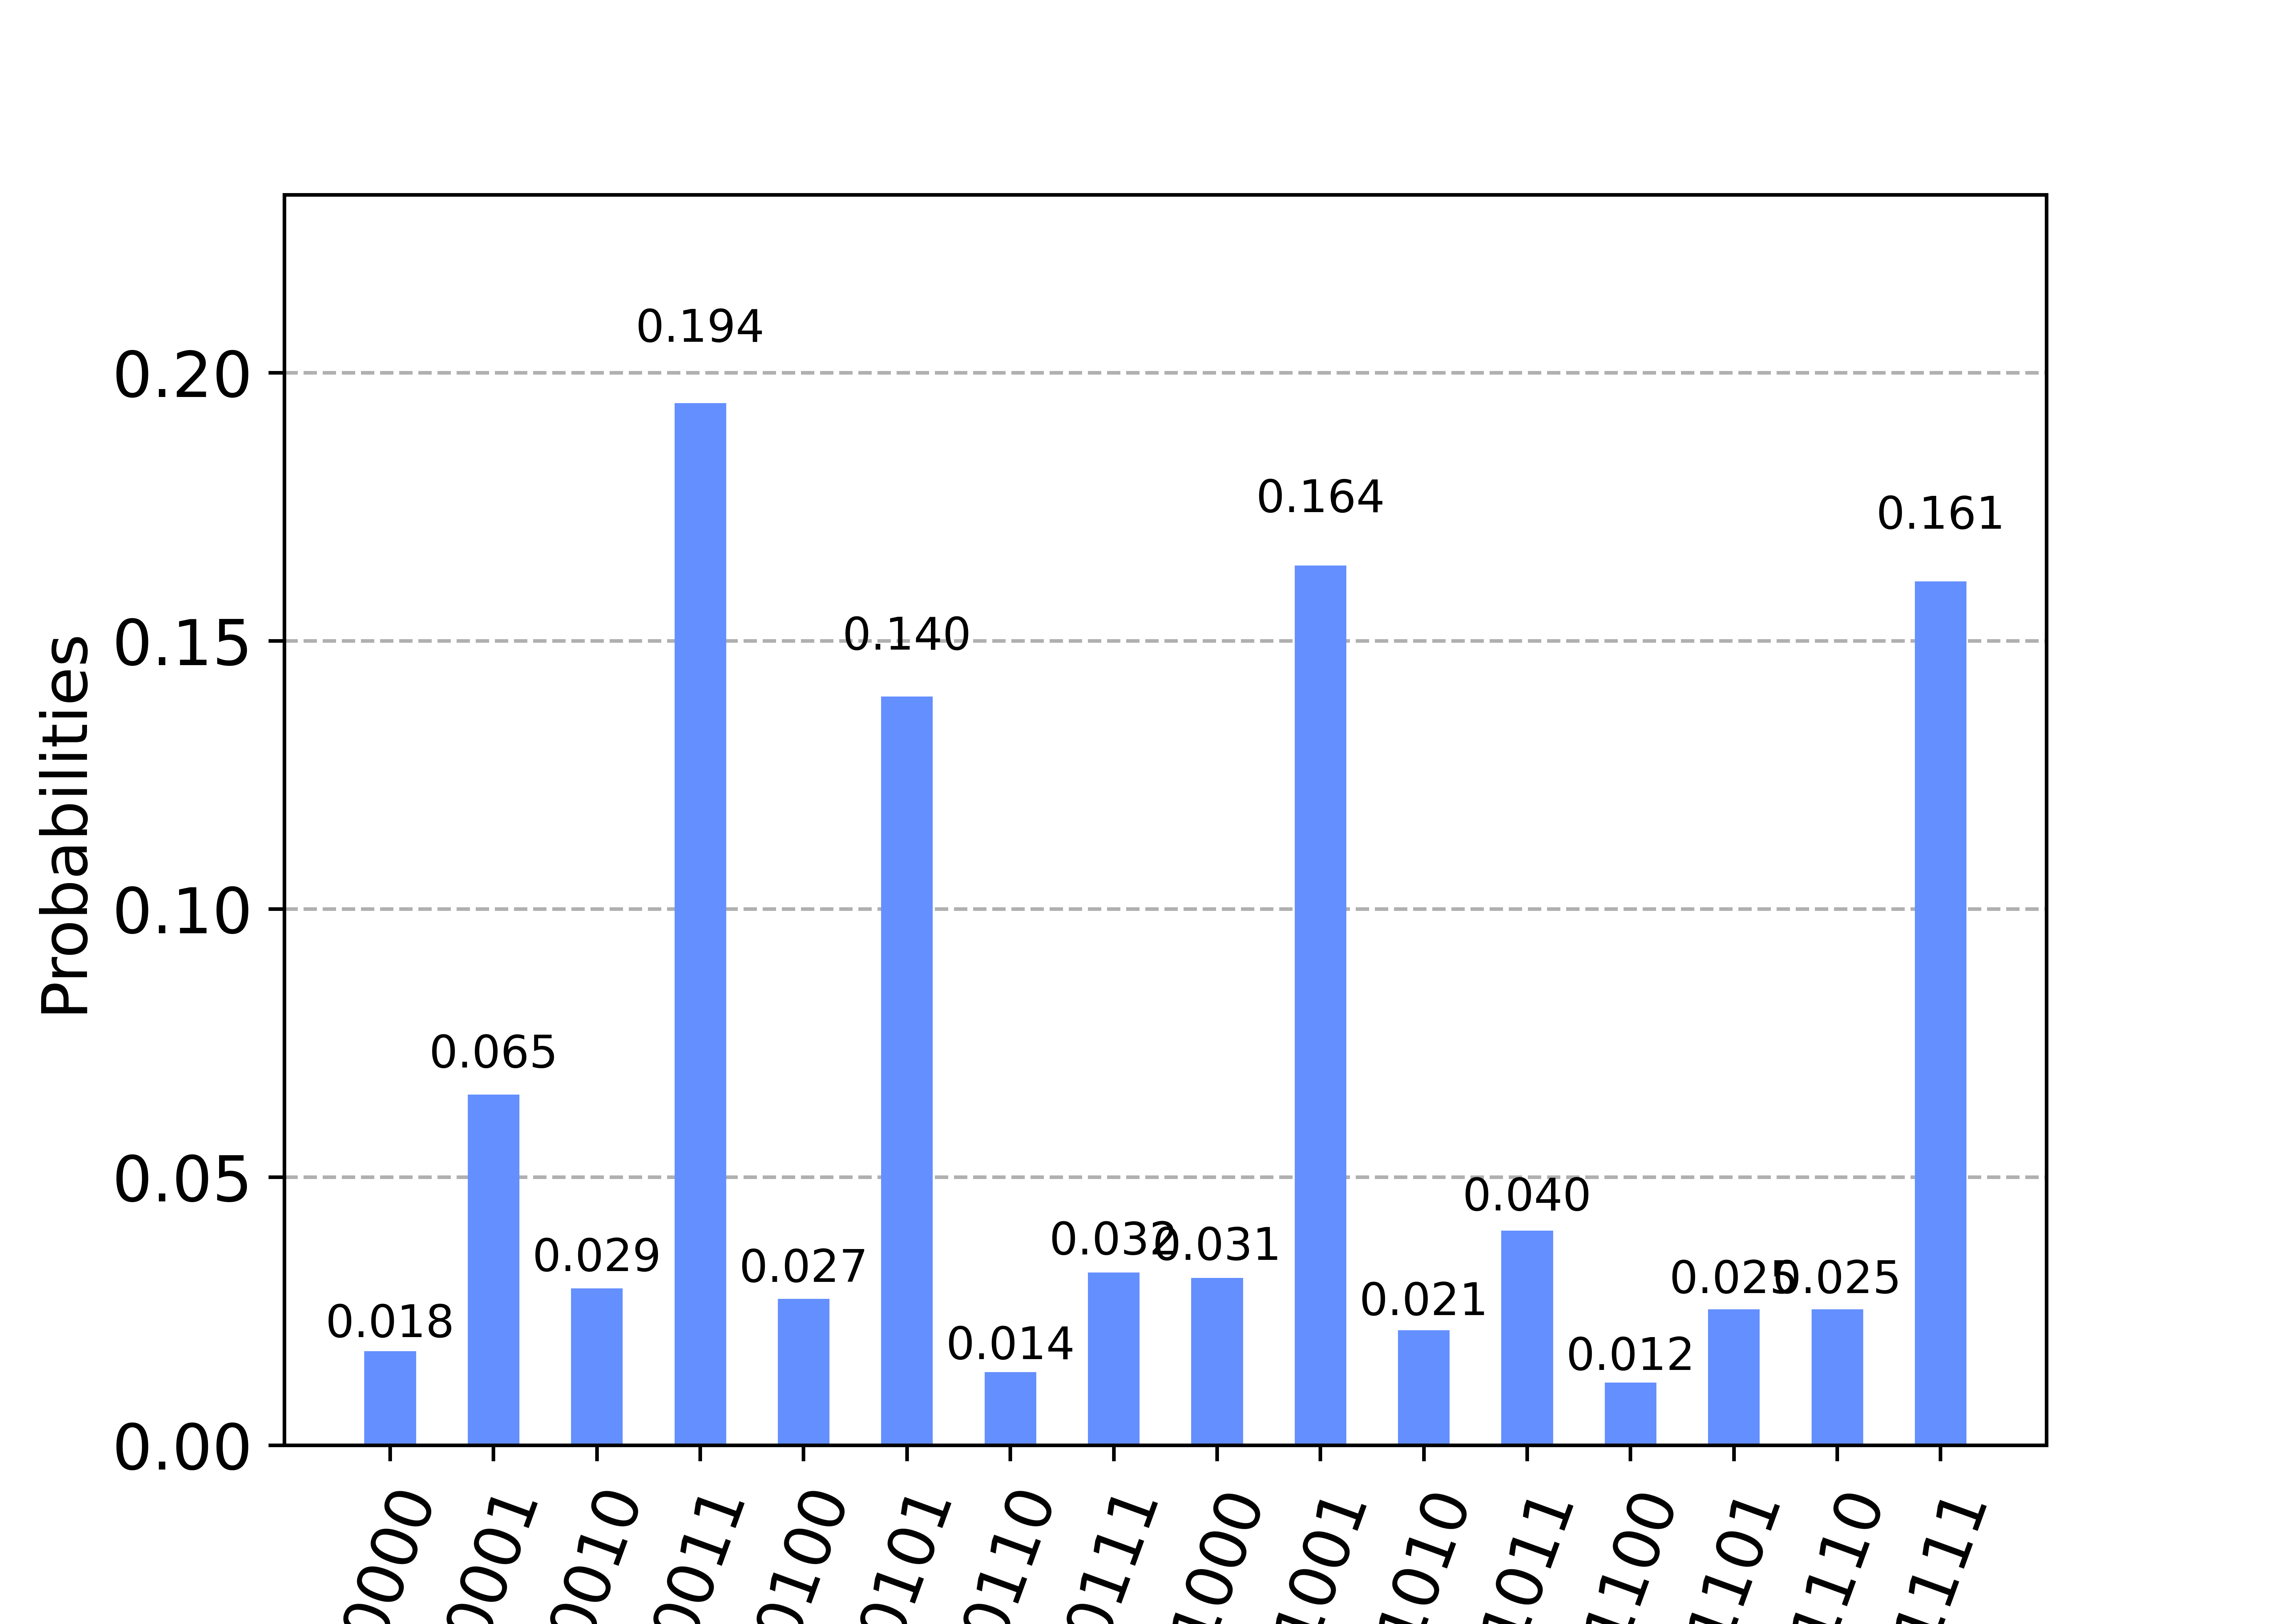
\includegraphics[width=\textwidth, height=.4\textheight, keepaspectratio]{custom_layout_results.png}
    \end{columns}
\end{frame}
\subsection{Analysis Pass}
{
\setbeamercolor{background canvas}{bg=black}
\setbeamercolor{footline}{fg=ibm}
\begin{frame}
    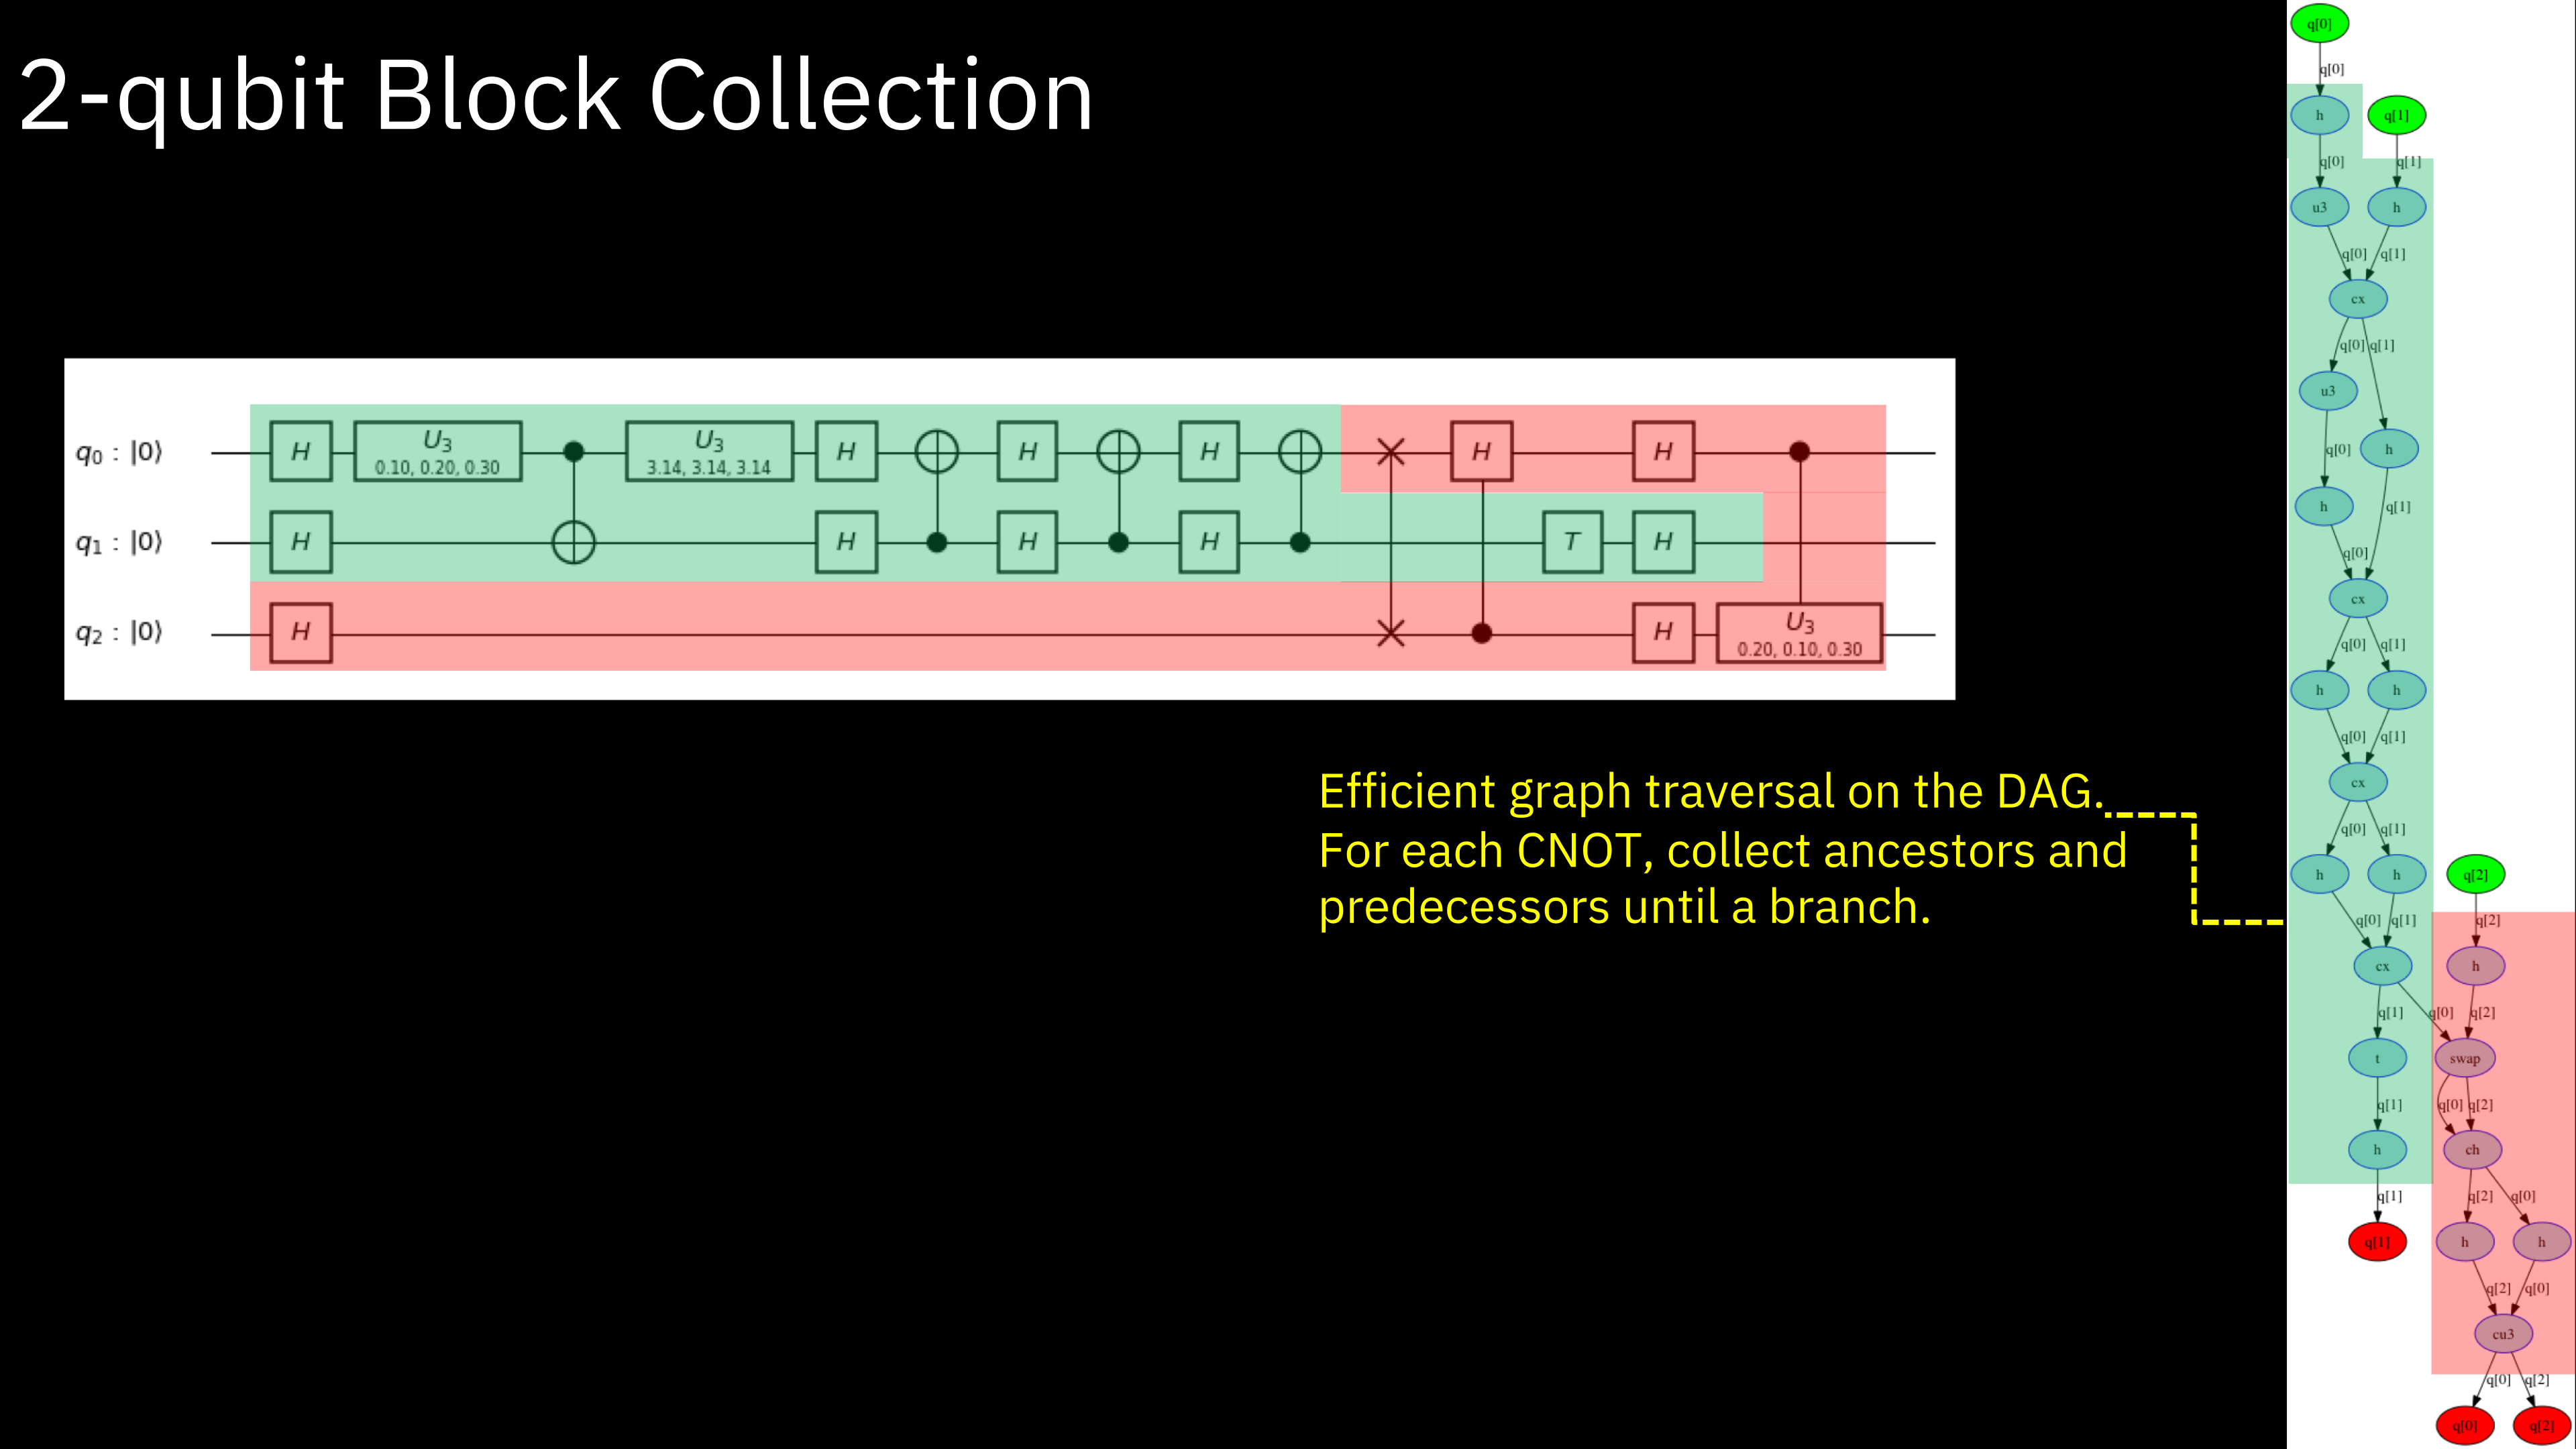
\includegraphics[width=\textwidth]{block_collection.png}
\end{frame}
}

\subsection{Optimization Passes}
\subsubsection{Consolidate Blocks}
\begin{frame}
    \frametitle{Consolidate Blocks}
    \begin{enumerate}
        \item Loop over 2Q blocks collecteds from analysis pass
        \item Run a simulation to find unitary matrix of each block
        \item Replace block with unitary matrix
    \end{enumerate}
    \begin{center}
    \vspace{3em}
    \only<1>{
        \begin{equation*}
            \Qcircuit @C=1.0em @R=1.0em @!R {
                \lstick{ {q0}_{0} : \ket{0} } & \multigate{1}{unitary} & \multigate{2}{unitary} & \qw & \qw\\
                \lstick{ {q0}_{1} : \ket{0} } & \ghost{unitary} & \ghost{unitary} & \qw & \qw\\
                \lstick{ {q0}_{2} : \ket{0} } & \qw & \ghost{unitary} & \qw & \qw\\
            }
        \end{equation*}
    }
    \only<2>{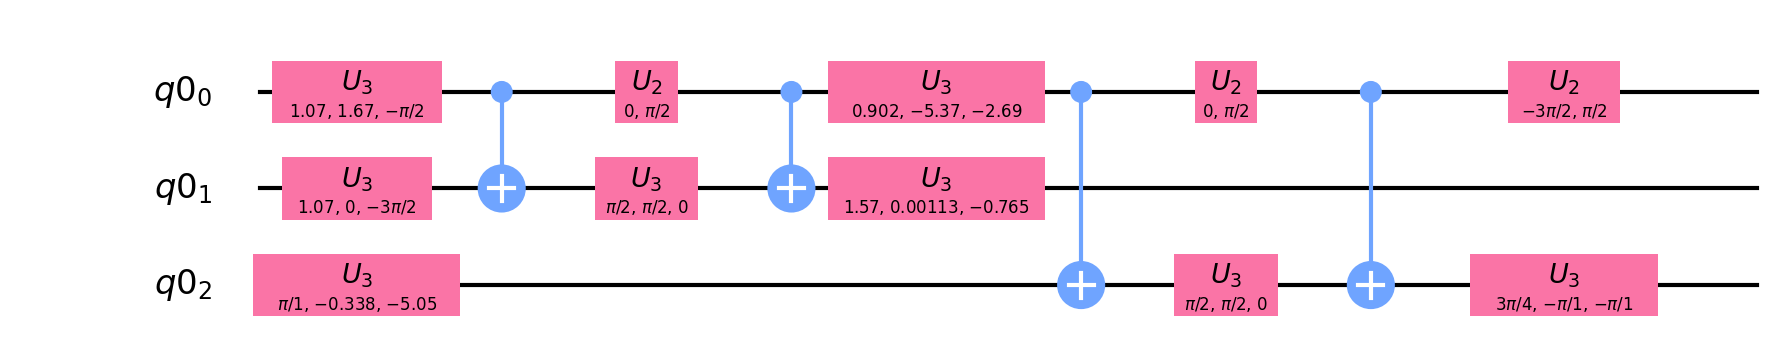
\includegraphics[width=\textwidth]{unrolled_unitary.png}}
\end{center}
\end{frame}

\subsubsection{Optimize 1Q operations}
\begin{frame}
    \frametitle{Optimize 1Q Operations}
    \begin{enumerate}
        \item Find all runs of 1Q operations on each Qubit in the dag
        \item For each run calculate the end state rotation
        \item Replace all 1Q operations with a single rotation gate to that end state
    \end{enumerate}
    \only<1> {
        \vspace{3em}
        \begin{equation*}
            \Qcircuit @C=1.0em @R=0.0em @!R {
	            \lstick{ {q}_{0} : \ket{0} } & \gate{H} & \gate{R_z(\frac{\pi}{4})} & \qw & \qw\\
    	    }
        \end{equation*}
    }
    \only<2> {
        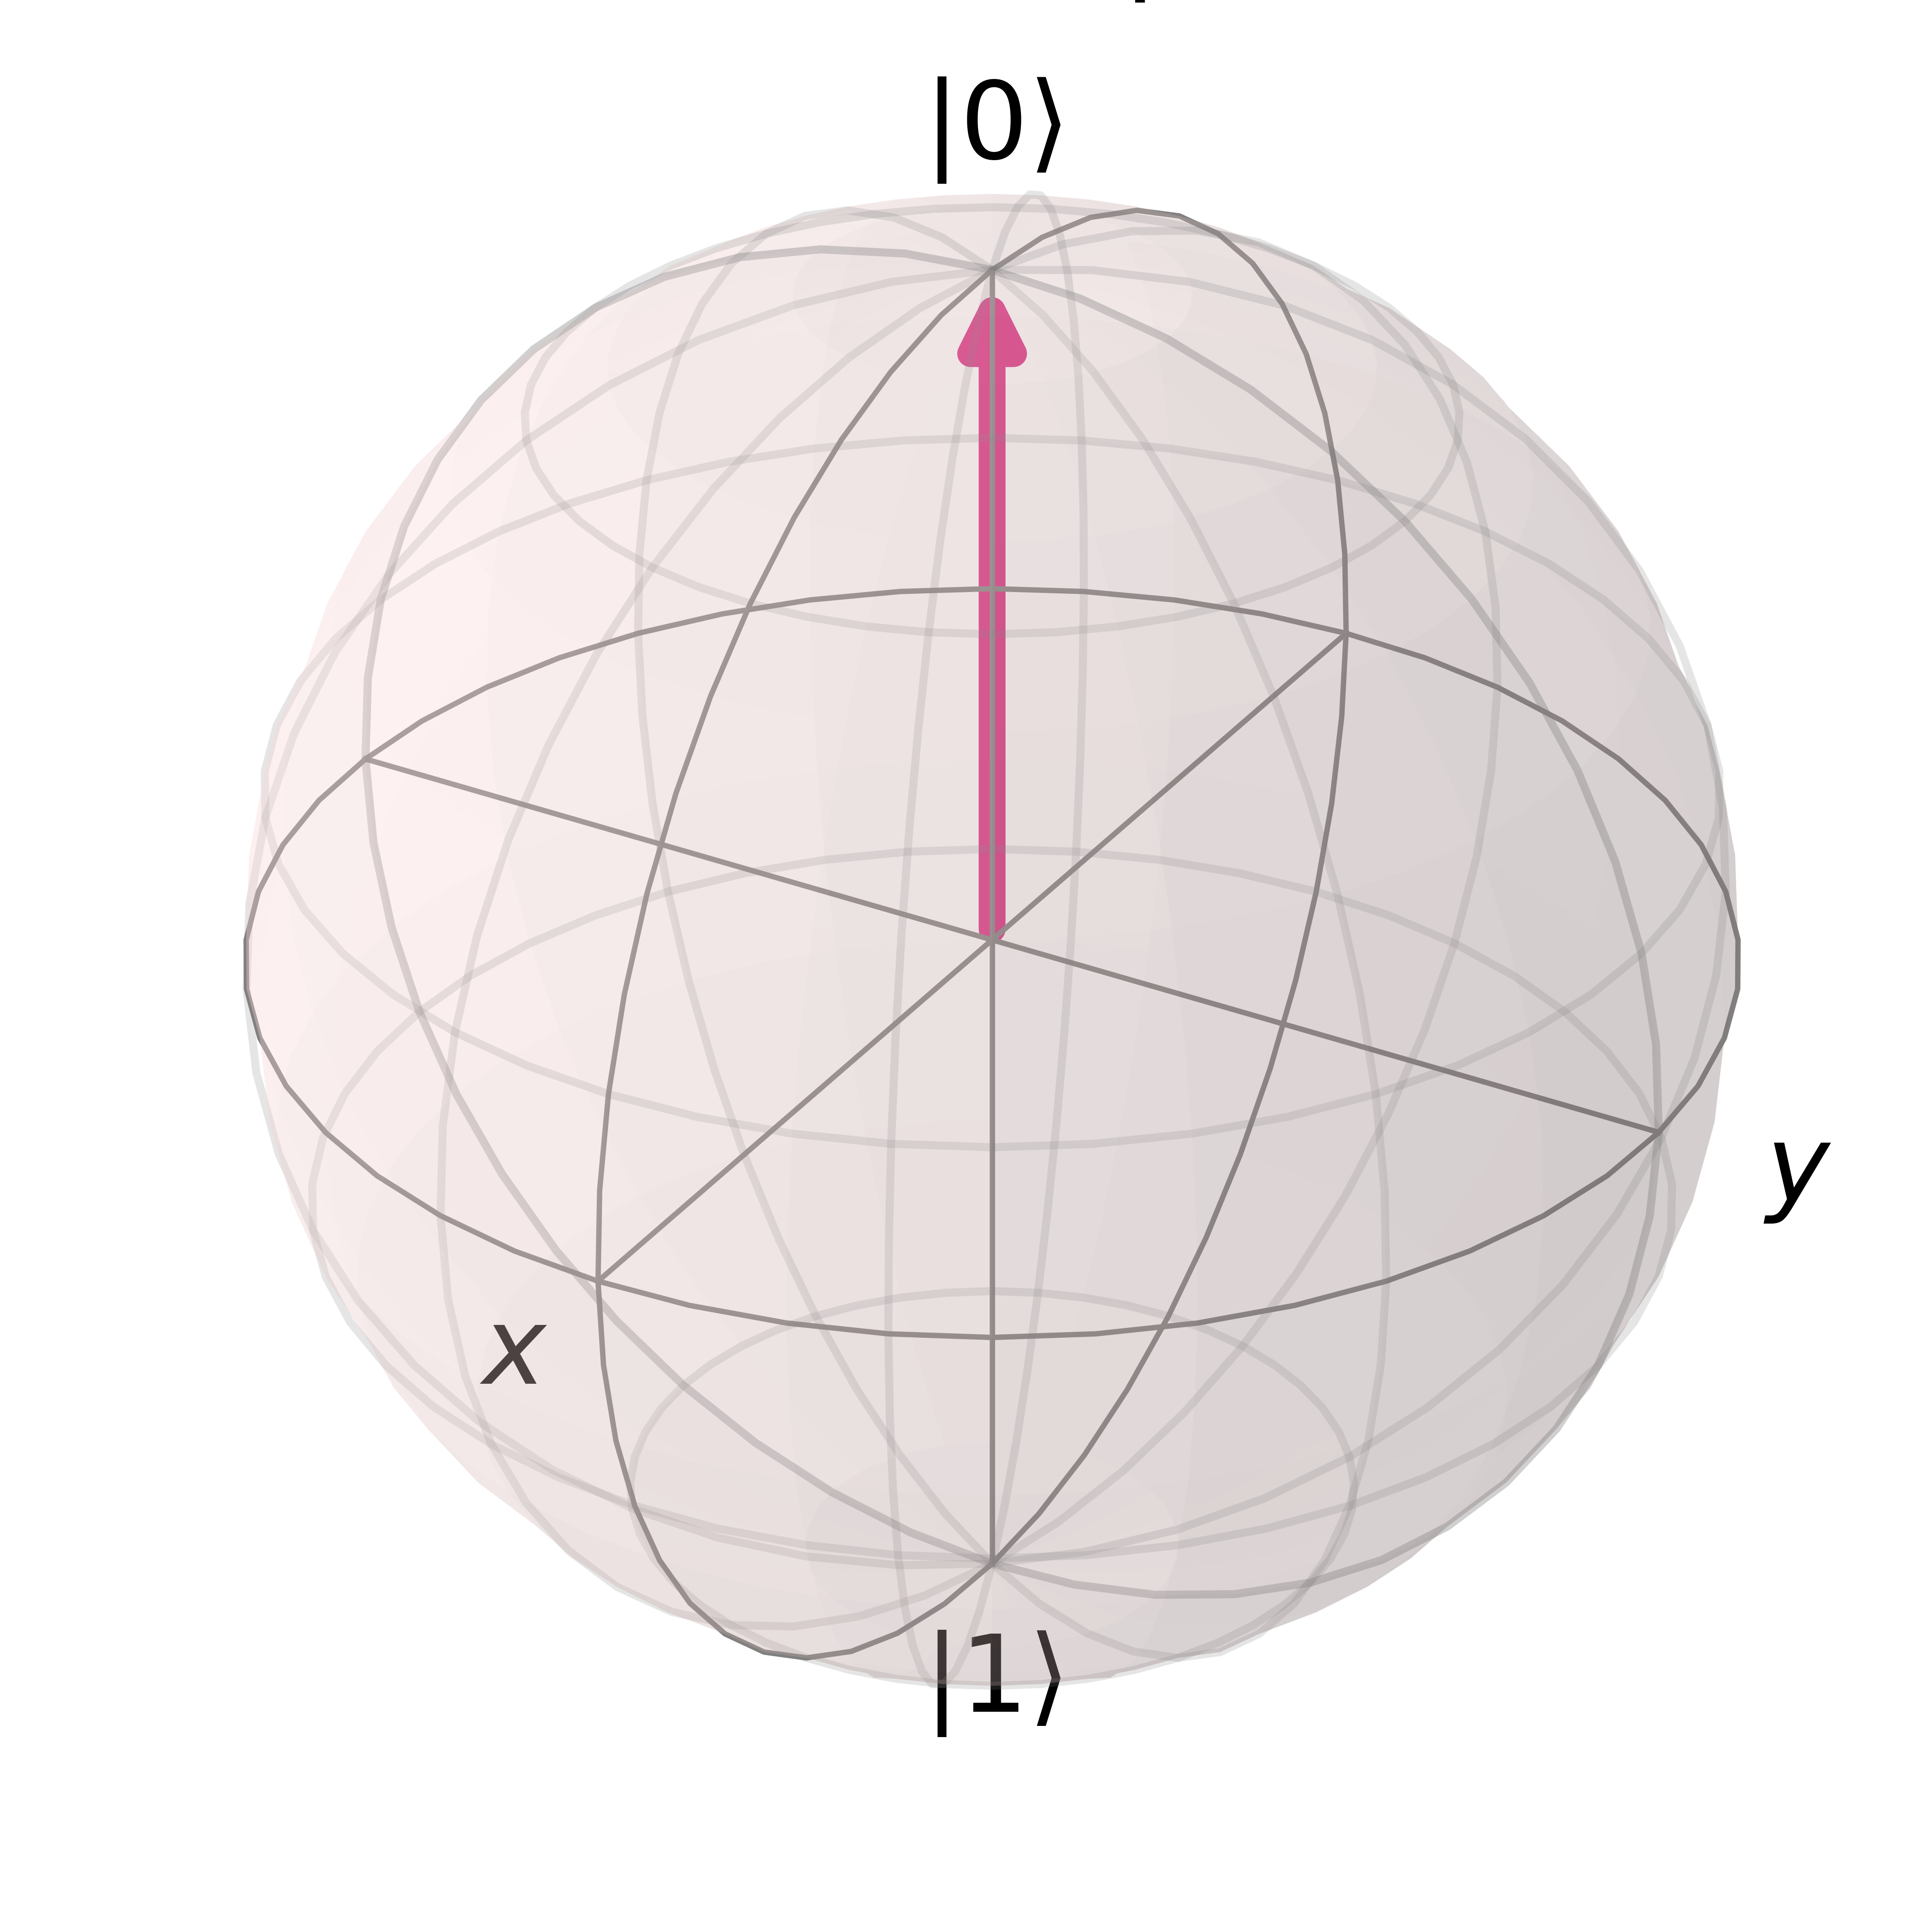
\includegraphics[width=.3\textwidth]{bloch_fresh.png} $\rightarrow$ 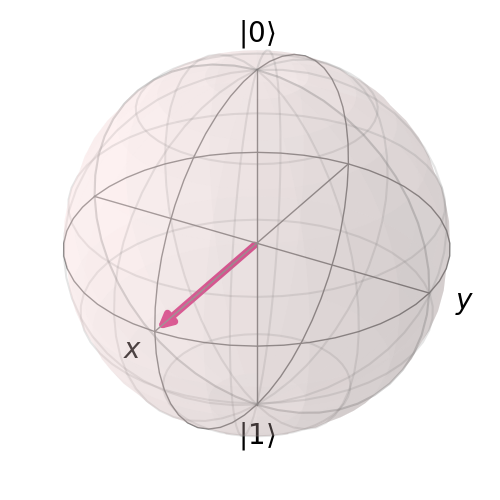
\includegraphics[width=.3\textwidth]{bloch_hadamard.png} $\rightarrow$ 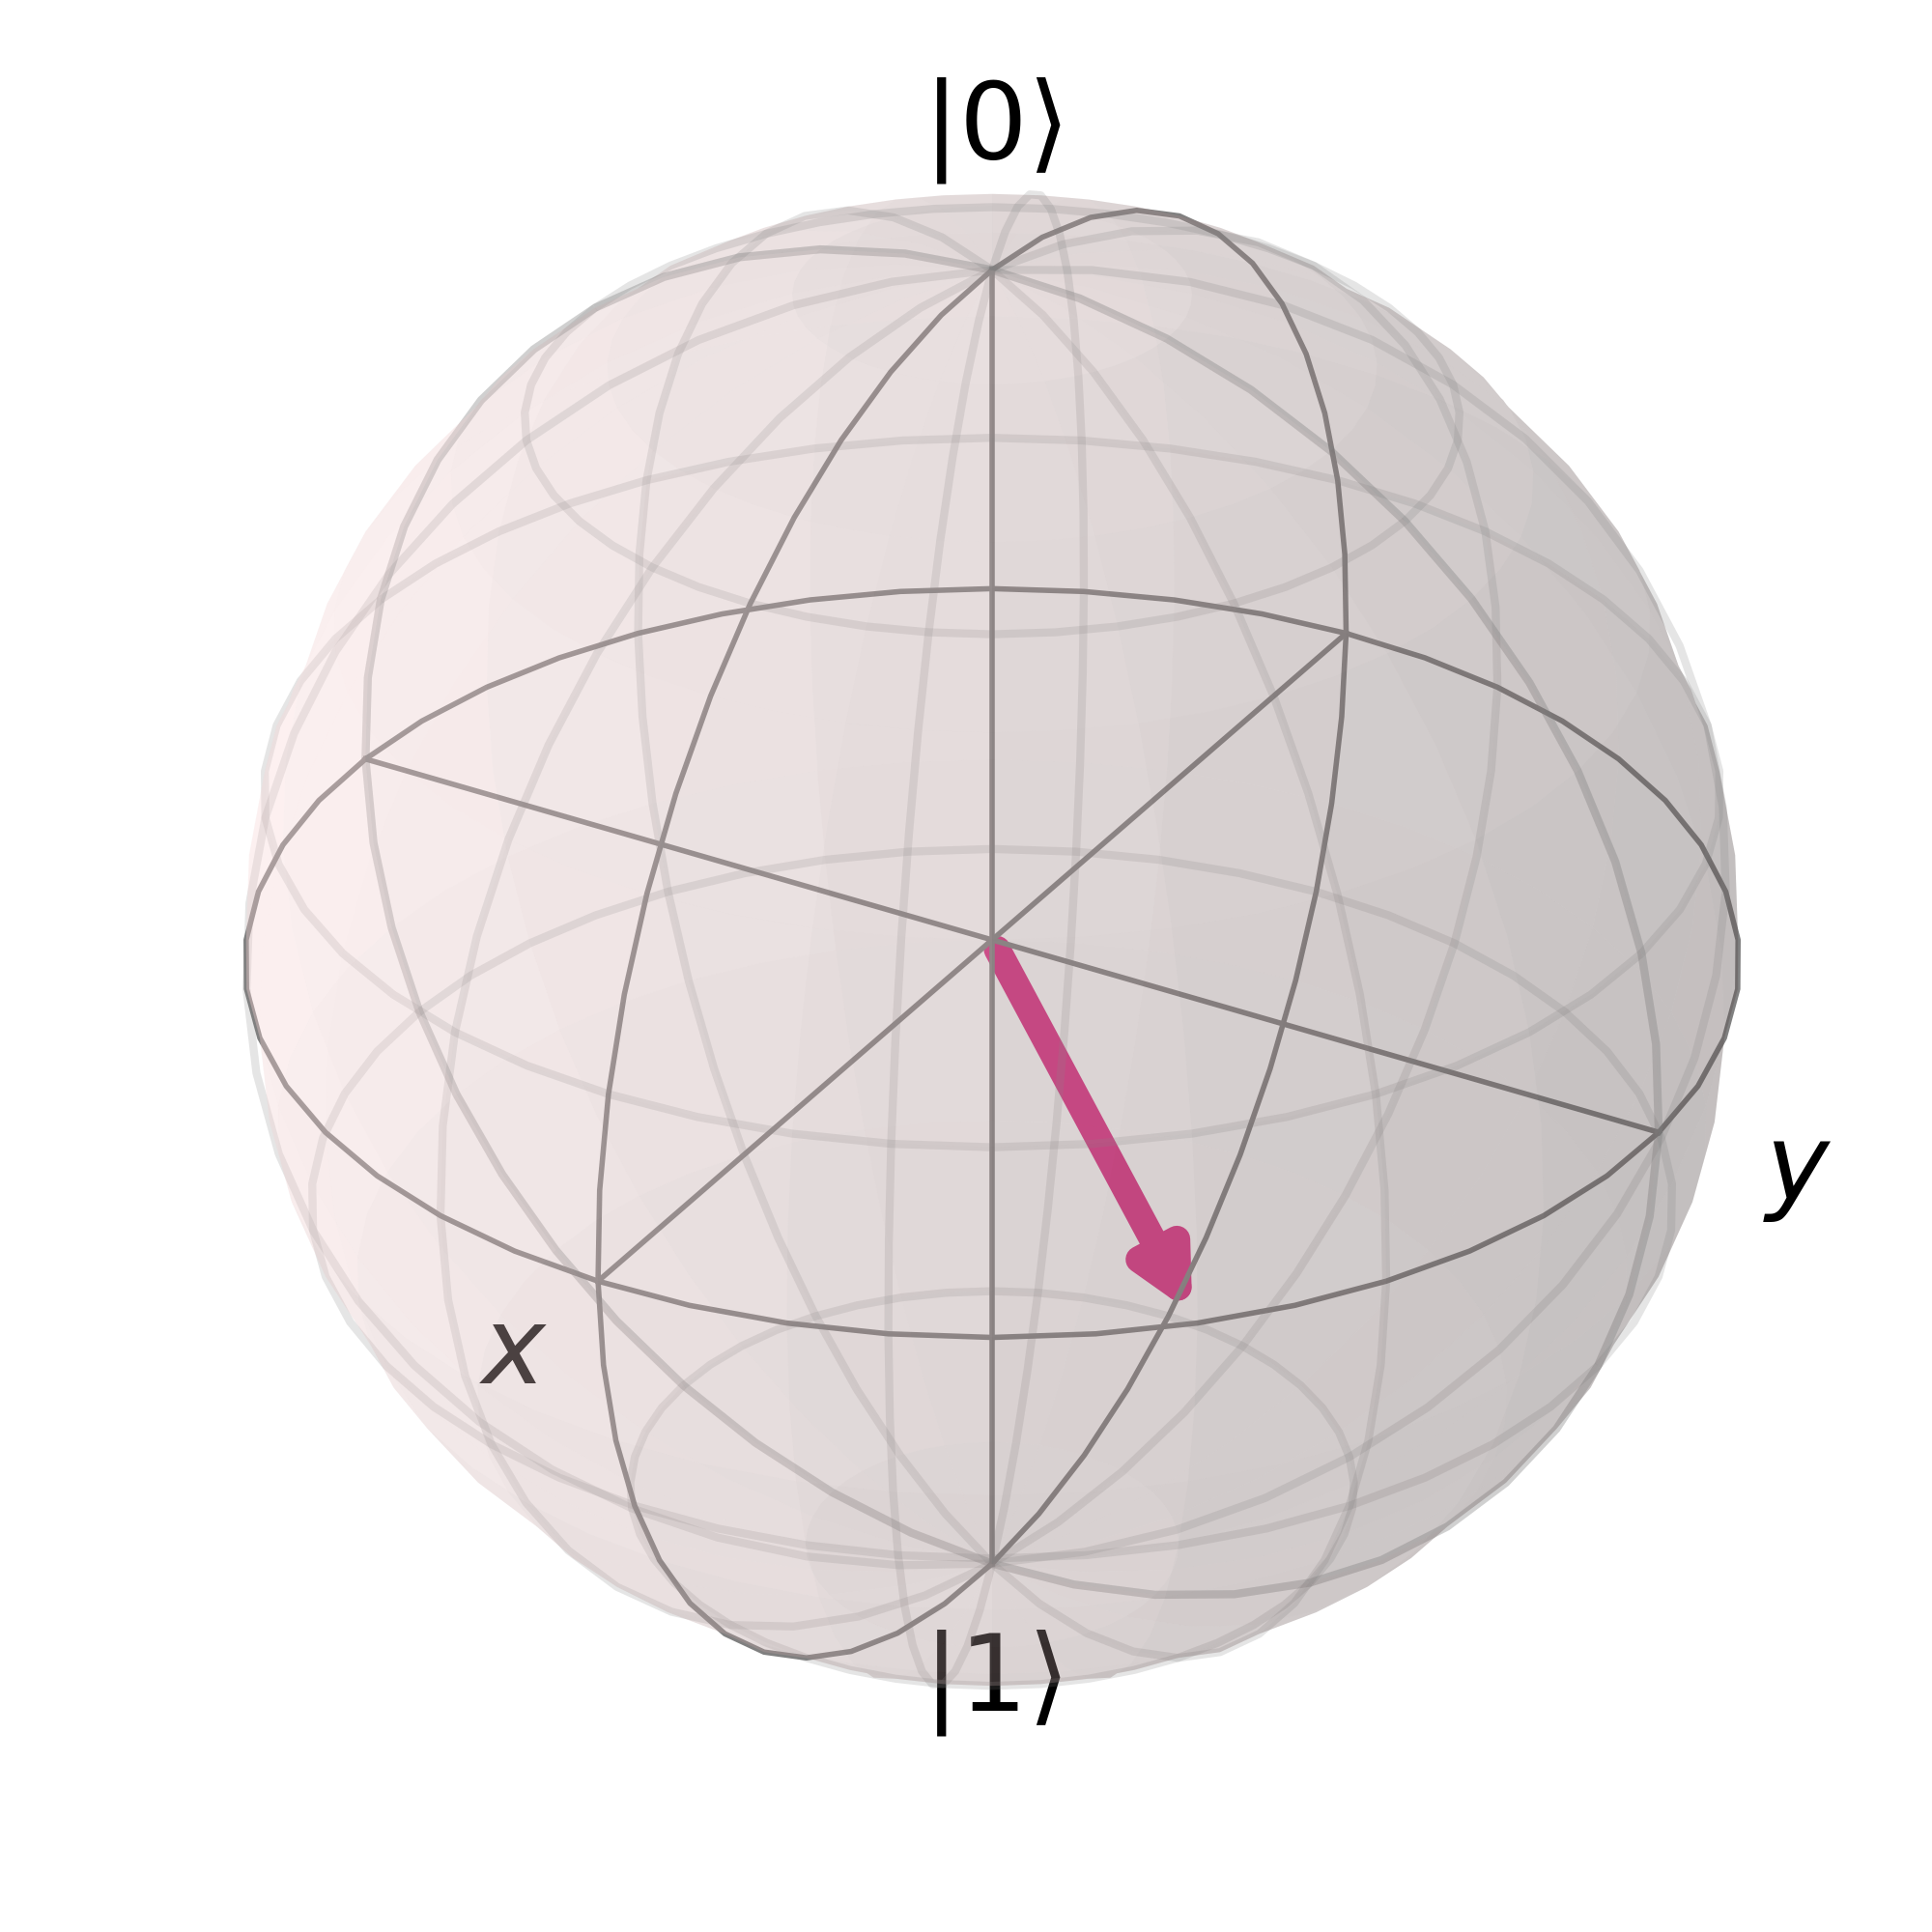
\includegraphics[width=.3\textwidth]{result_1q_bloch.png}
    }
    \only<3> {
        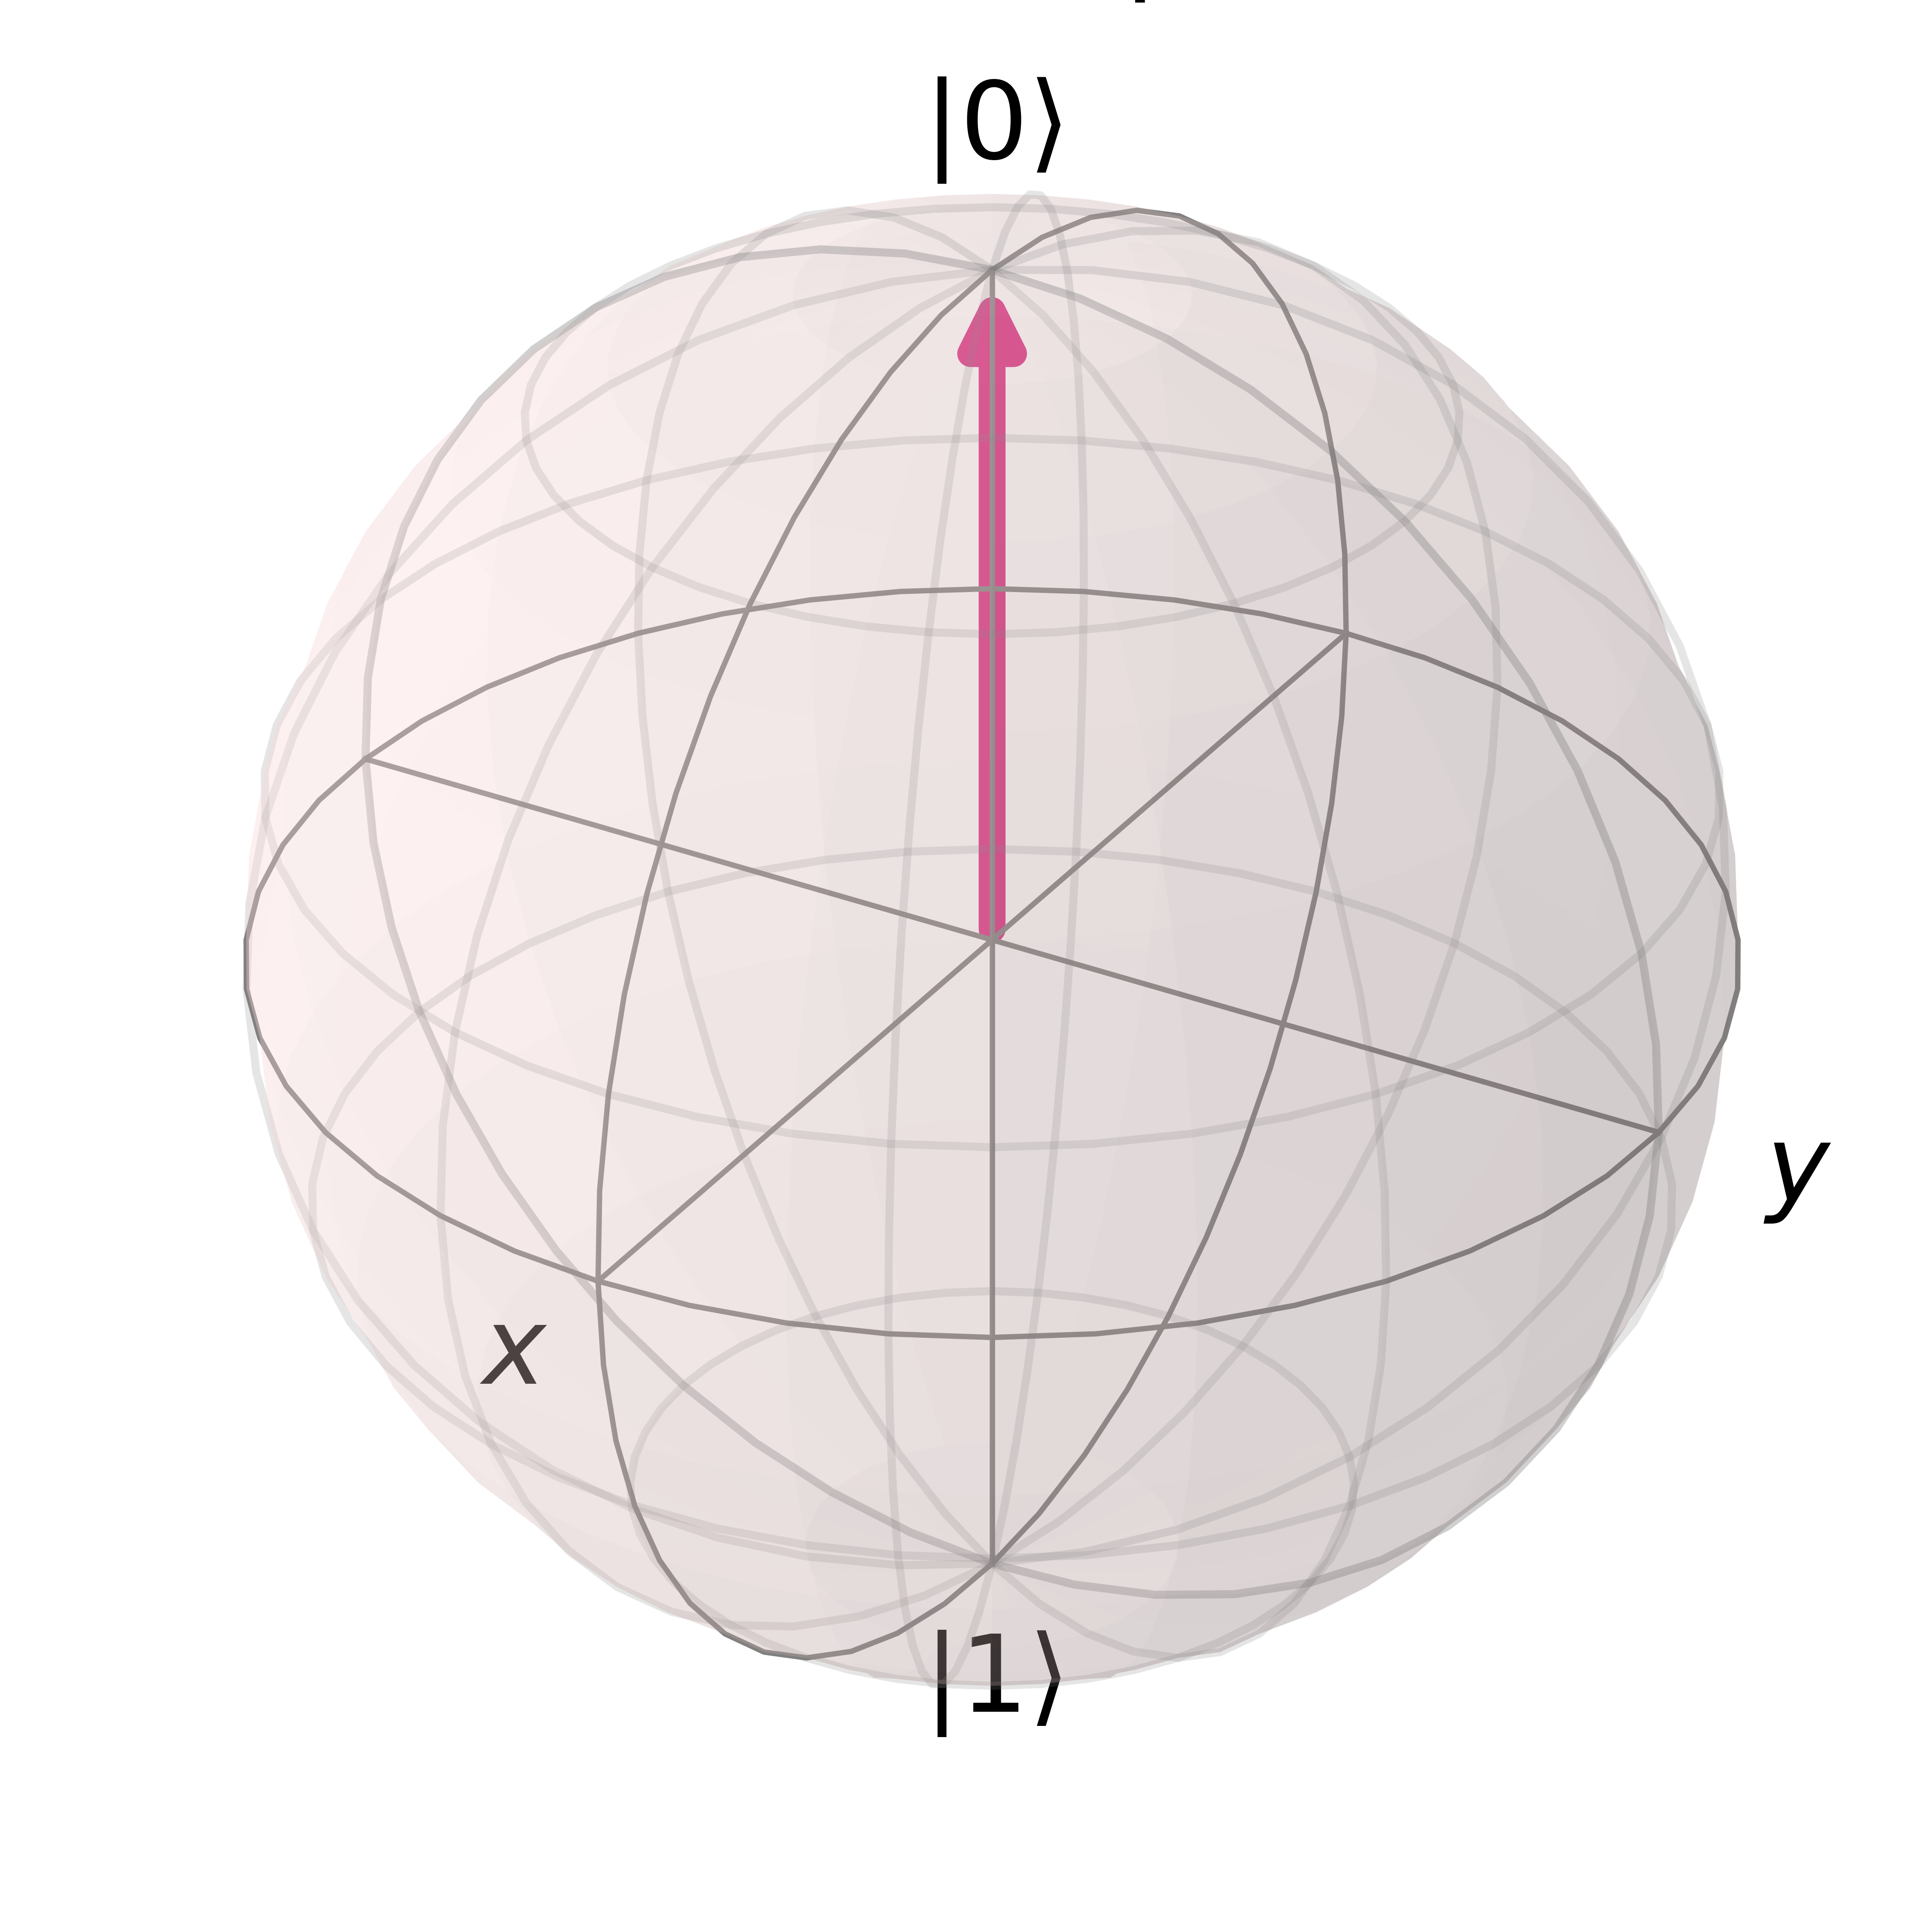
\includegraphics[width=.45\textwidth]{bloch_fresh.png} $\rightarrow$ 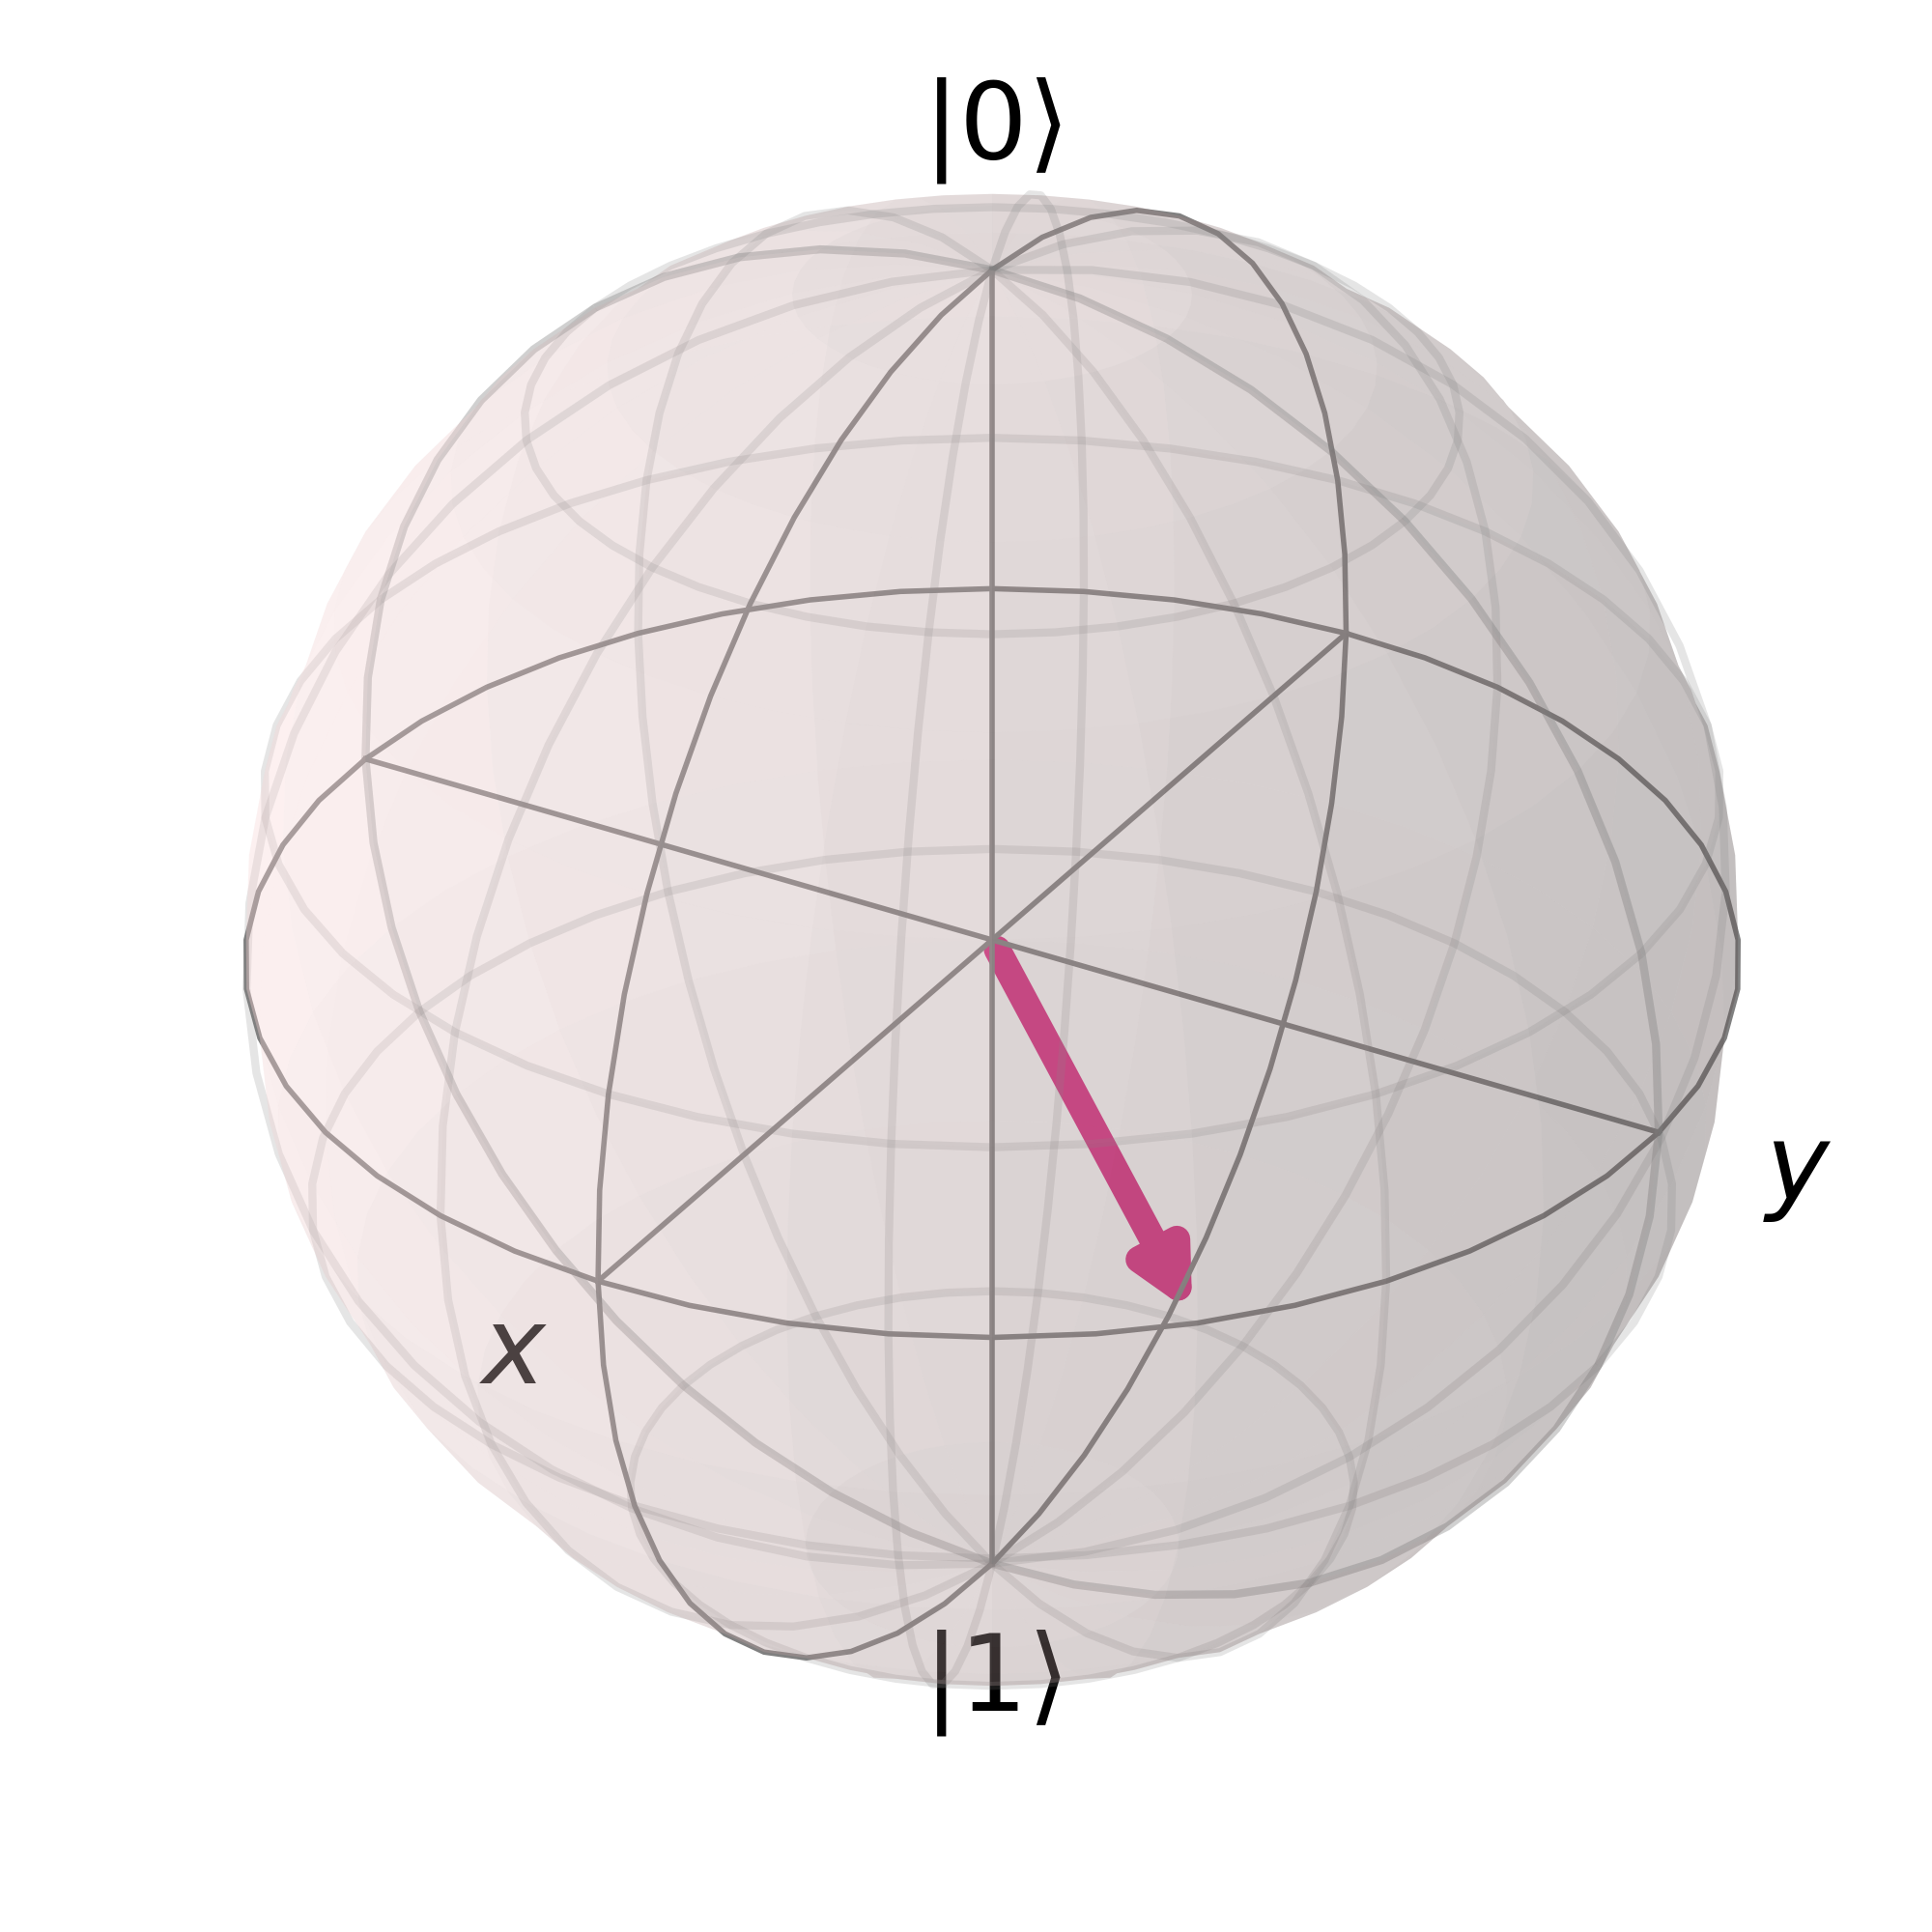
\includegraphics[width=.45\textwidth]{result_1q_bloch.png}
    }
    \only<4> {
        \vspace{3em}
        \begin{equation*}
            \Qcircuit @C=1.0em @R=0.0em @!R {
        	 	\lstick{ {q}_{0} : \ket{0} } & \gate{U_2\left(\frac{\pi}{4},\pi\right)} & \qw & \qw\\
            }
        \end{equation*}
    }

\end{frame}

\subsection{Device Mapping}
\begin{frame}
    \frametitle{Swap Mapping/Routing}
    \begin{columns}
        \column{.5\textwidth}
            \begin{itemize}
                \item After the layout step we need to ensure that 
                \item 3 Algorithms included in Qiskit
                    \begin{itemize}
                        \item \href{https://github.com/Qiskit/qiskit-terra/blob/master/qiskit/transpiler/passes/routing/basic_swap.py}{BasicSwap}
                        \item \href{https://github.com/Qiskit/qiskit-terra/blob/master/qiskit/transpiler/passes/routing/lookahead_swap.py}{LookaheadSwap}
                        \item \href{https://github.com/Qiskit/qiskit-terra/blob/master/qiskit/transpiler/passes/routing/stochastic_swap.py}{StochasticSwap}
                    \end{itemize}
                \item StochasticSwap is used in all presets
            \end{itemize}
        \column{.5\textwidth}
            Insert Diagram of Swap Mapping
    \end{columns}
        
\end{frame}

\section{Conclusions}
\subsection{Quantum Volume}
{
\setbeamercolor{background canvas}{bg=black}
\setbeamercolor{footnote}{fg=ibm}
\setbeamercolor{footnote mark}{fg=ibm}
\setbeamercolor{footline}{fg=ibm}
\begin{frame}
    \frametitle{Quantum Volume\footnotemark[1]}
    \begin{center}
        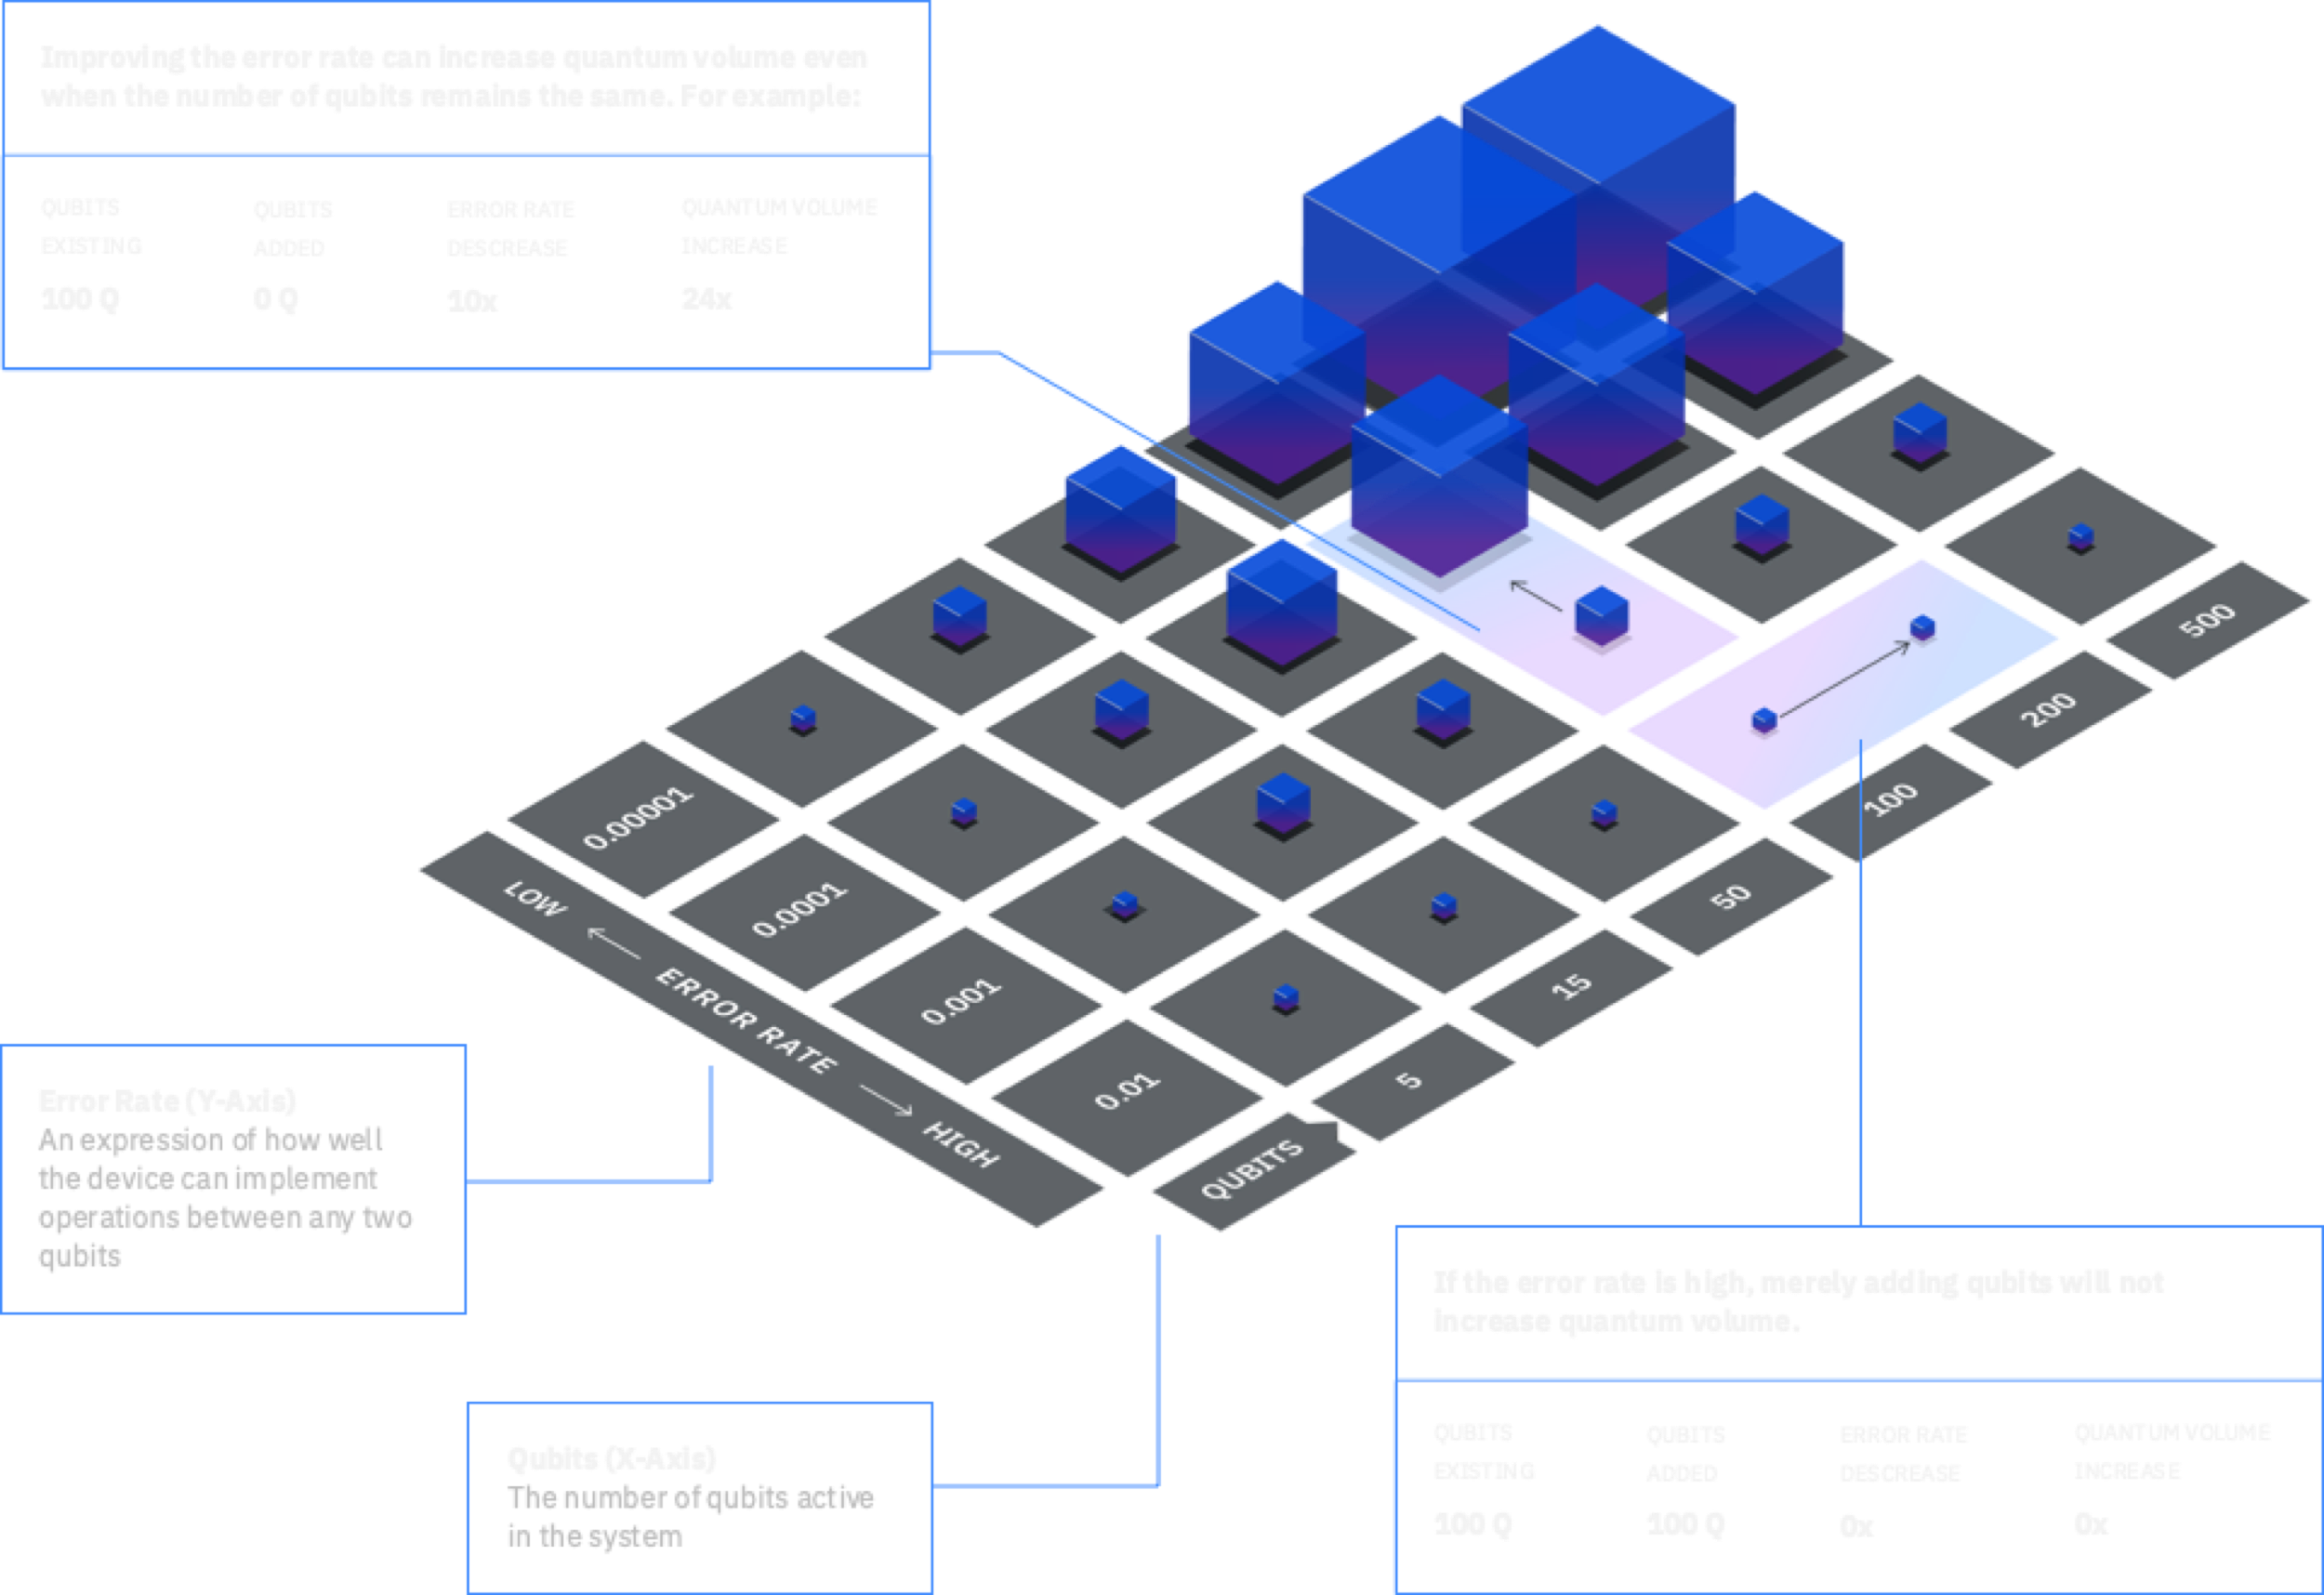
\includegraphics[width=\textwidth,height=.8\textheight,keepaspectratio]{qv.png}
    \end{center}
    \footnotetext[1]{\href{https://arxiv.org/abs/1811.12926}{https://arxiv.org/abs/1811.12926}}
\end{frame}
}

\begin{frame}
    \frametitle{Conclusions}
    \begin{itemize}
        \item Techniques used are similar to a classical compiler
        \item Implementation details are different because of uniqueness of quantum computing
        \item A good compiler can be the difference between a functional
            program and one that doesn't work
    \end{itemize}
\end{frame}

\section{Questions?}
\begin{frame}
\frametitle{Where to get more information}
    \begin{itemize}
        \item These Slides: \href{https://github.com/mtreinish/quantum-compilers}{https://github.com/mtreinish/quantum-compilers}
        \item Qiskit: \href{https://qiskit.org/}{https://qiskit.org/}
        \item Qiskit Terra on Github: \href{https://github.com/Qiskit/qiskit-terra}{https://github.com/Qiskit/qiskit-terra}
        \item IBM Q Experience (sign up to get access to public quantum computers): \href{https://quantum-computing.ibm.com}{https://quantum-computing.ibm.com}
        \item Tutorial on using Passmanager: {\small \href{https://github.com/Qiskit/qiskit-iqx-tutorials/blob/master/qiskit/advanced/terra/4\_transpiler\_passes\_and\_passmanager.ipynb}{https://github.com/Qiskit/qiskit-iqx-tutorials/blob/master/qiskit/advanced/terra/4\_transpiler\_passes\_and\_passmanager.ipynb}}
        \item Qiskit Textbook: \href{https://qiskit.org/textbook/}{https://qiskit.org/textbook/}
    \end{itemize}
\end{frame}

%\section{Backup Slides}
%\begin{frame}[noframenumbering]
%    \frametitle{BACKUP SLIDES}
%\end{frame}

\end{document}
